%
All profile likelihood fits are performed using TRExFitter version 00-04-16. In the control regions, the fit is performed over the HT distribution. In the signal regions, the fit is performed over the distribution of an MVA output. 2 different MVA’s are separately evaluated: a BDT similar to that used in the SM4top analysis (see section \ref{sec:mva_bdt}), and a GNN developed for this analysis (see section \ref{sec:mva_gnn}). For each of the 2 MVA’s, 2 versions are used: an MVA optimized for the 1L final state, and an MVA optimized for the 2LOS final state. Therefore the complete examination of the 1LOS combined channel fits includes 2 different fits that each incorporate 2 different trained MVA’s for each mass point (each MVA is trained separately for each mass point). The baseline MVA is GNN, and all results in this section use GNN output distribtuions in the fit, unless stated otherwise.

Asimov pseudodata matching the nominal predicted yields is used, and the fit is performed on both control region and signal region distributions. The signal strength parameter $\mu$ is kept free-floating with an initial value of 0. Given that the Asimov fit assumes exact accuracy of the pseudodata, which is not true, the significance and limit values output from this fit are not conclusive. Rather, they can be used as a point of comparison with which to optimize the analysis strategy. The Asimov fit cannot alter the values of the systematics, but it can constrain their possible range.

The pre-fit distributions associated with each region are shown in Figure \ref{fig:Prefit_Yields_1L} for 1L and Figure \ref{fig:Prefit_Yields_2L} for 2LOS. The signal regions contain GNN output distribution trained for mH=400\gev in these plots. The nuisance parameter constraints are compared between 1L, 2LOS, and the combined fit in Figures \ref{fig:Plain_NP_instrumental}-\ref{fig:Plain_NP_other}. The largest constraints are on \ttbar modeling parameters such as $t\bar{t}$+2b 4FS. This systematic uncertainty is also the most dominant uncertainty, as shown in the ranking plots in Figure \ref{fig:Ranking_mH400_Asimov} (mH=400\gev), Figure \ref{fig:Ranking_mH700_Asimov} (mH=700\gev), and Figure \ref{fig:Ranking_mH1000_Asimov} (mH=1000\gev).
% Missing emu channel, irrelevant now
%Figure \ref{fig:Ranking_mH400_Asimov_BDT} shows the ranking for mH=400\gev from fits using BDT output distribution in the signal regions (all the previous rankings use GNN). For the fit using 2L regions, the most dominant systematic uncertainty is again $t\bar{t}$+2b PS, although it is not so much dominant as in the fit on GNN distributions. This is also not understood.

The correlation matrices for the 1L, 2LOS, and combined fit systematics are shown in Figure \ref{fig:Corr_mH400_Asimov_1L}, Figure \ref{fig:Corr_mH400_Asimov_2L}, and Figure \ref{fig:Corr_mH400_Asimov_all} respectively.

The expected exclusion limits for all assumed Higgs Boson mass in the range of [400,1000] was found to be 20-10\%  better with the GNN discriminant for both lepton decay channels, resulting in better analysis sensitivity(see Appendix \ref{app:BDTvsGNN}) as compared to BDT. Hence, results using GNN discriminant are used in analysis as a baseline.


\begin{figure}[htbp!]
        \begin{center} \setlength{\tabcolsep}{2.5pt}\footnotesize
        \begin{tabular}{cccc}
        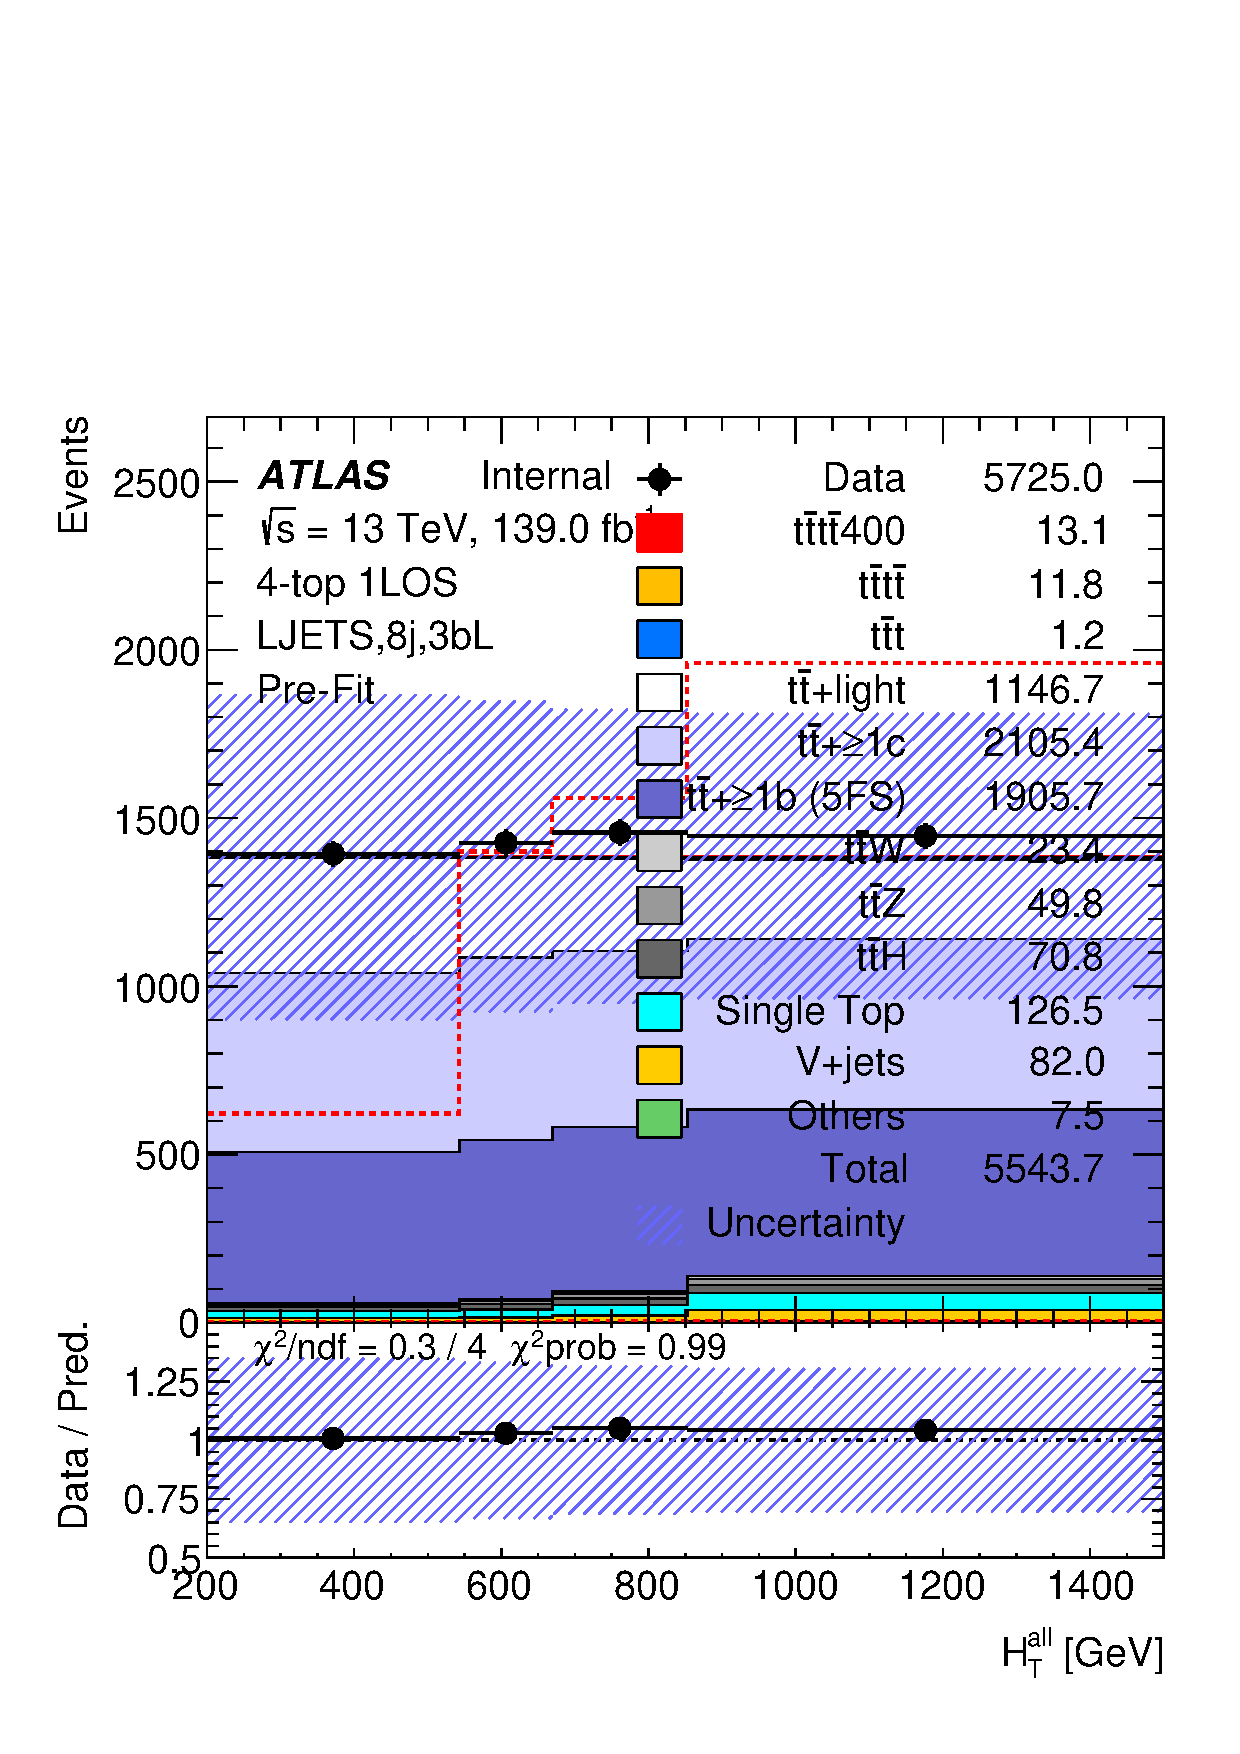
\includegraphics[width=0.23 \textwidth]{figures/fits/GNN/400/1L/data_unblindedSplusB/Plots/ljets_8j3bL.pdf} &
        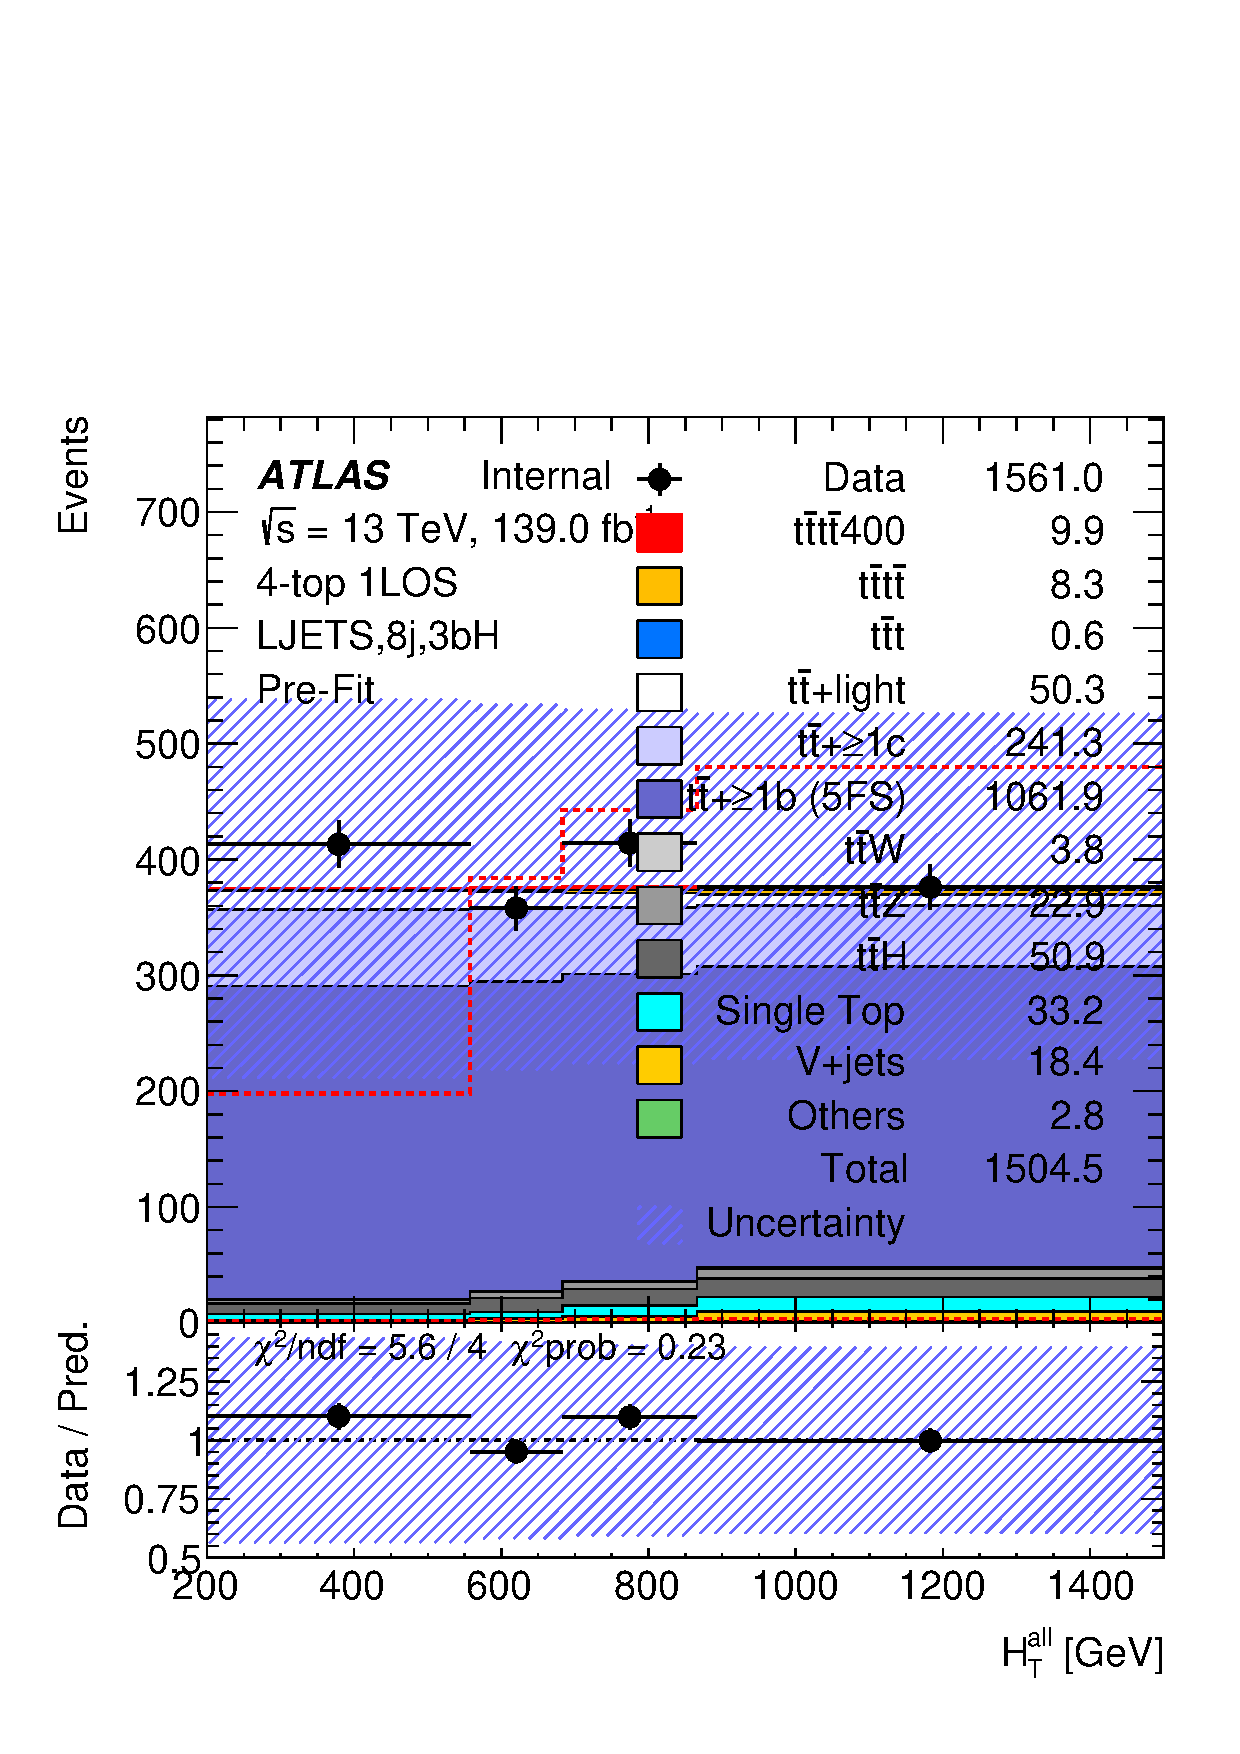
\includegraphics[width=0.23 \textwidth]{figures/fits/GNN/400/1L/data_unblindedSplusB/Plots/ljets_8j3bH.pdf} &
        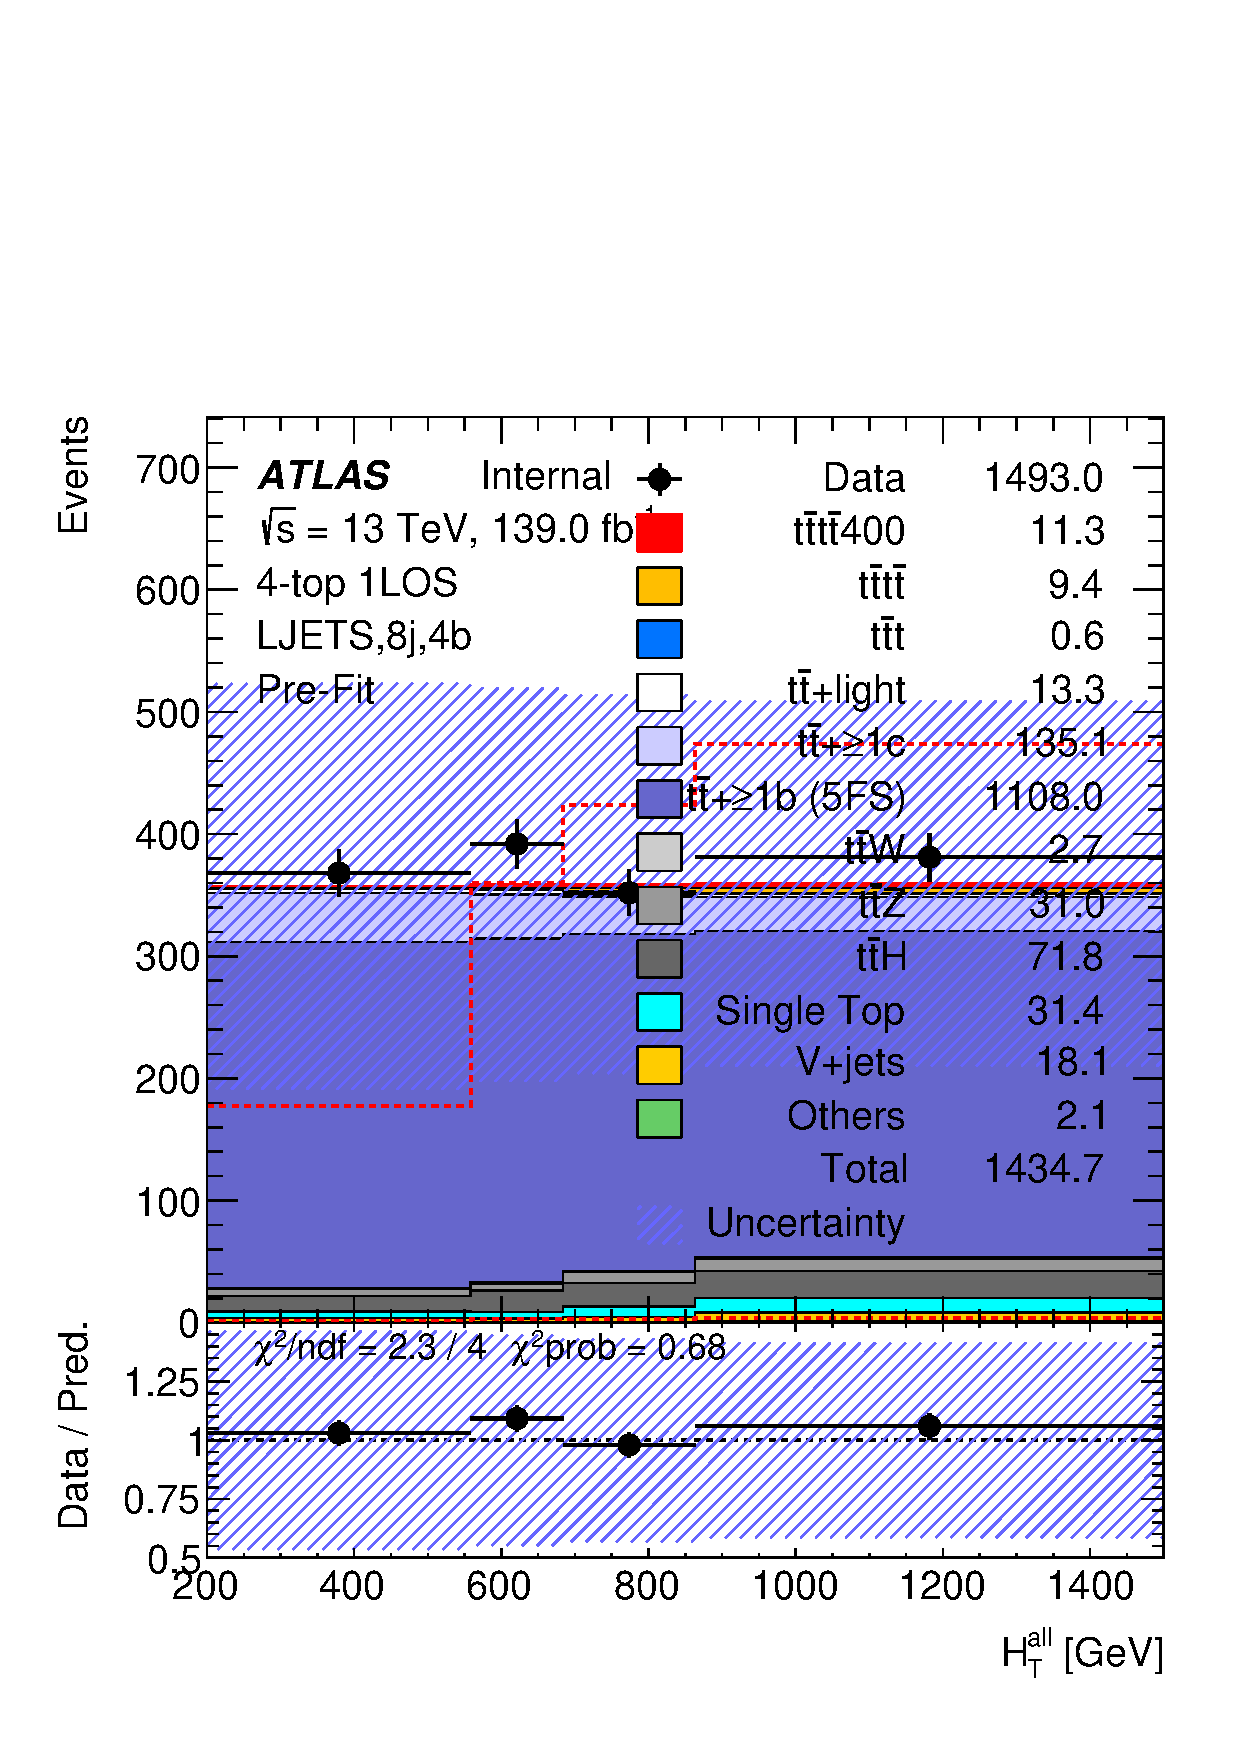
\includegraphics[width=0.23 \textwidth]{figures/fits/GNN/400/1L/data_unblindedSplusB/Plots/ljets_8j4b.pdf} &
        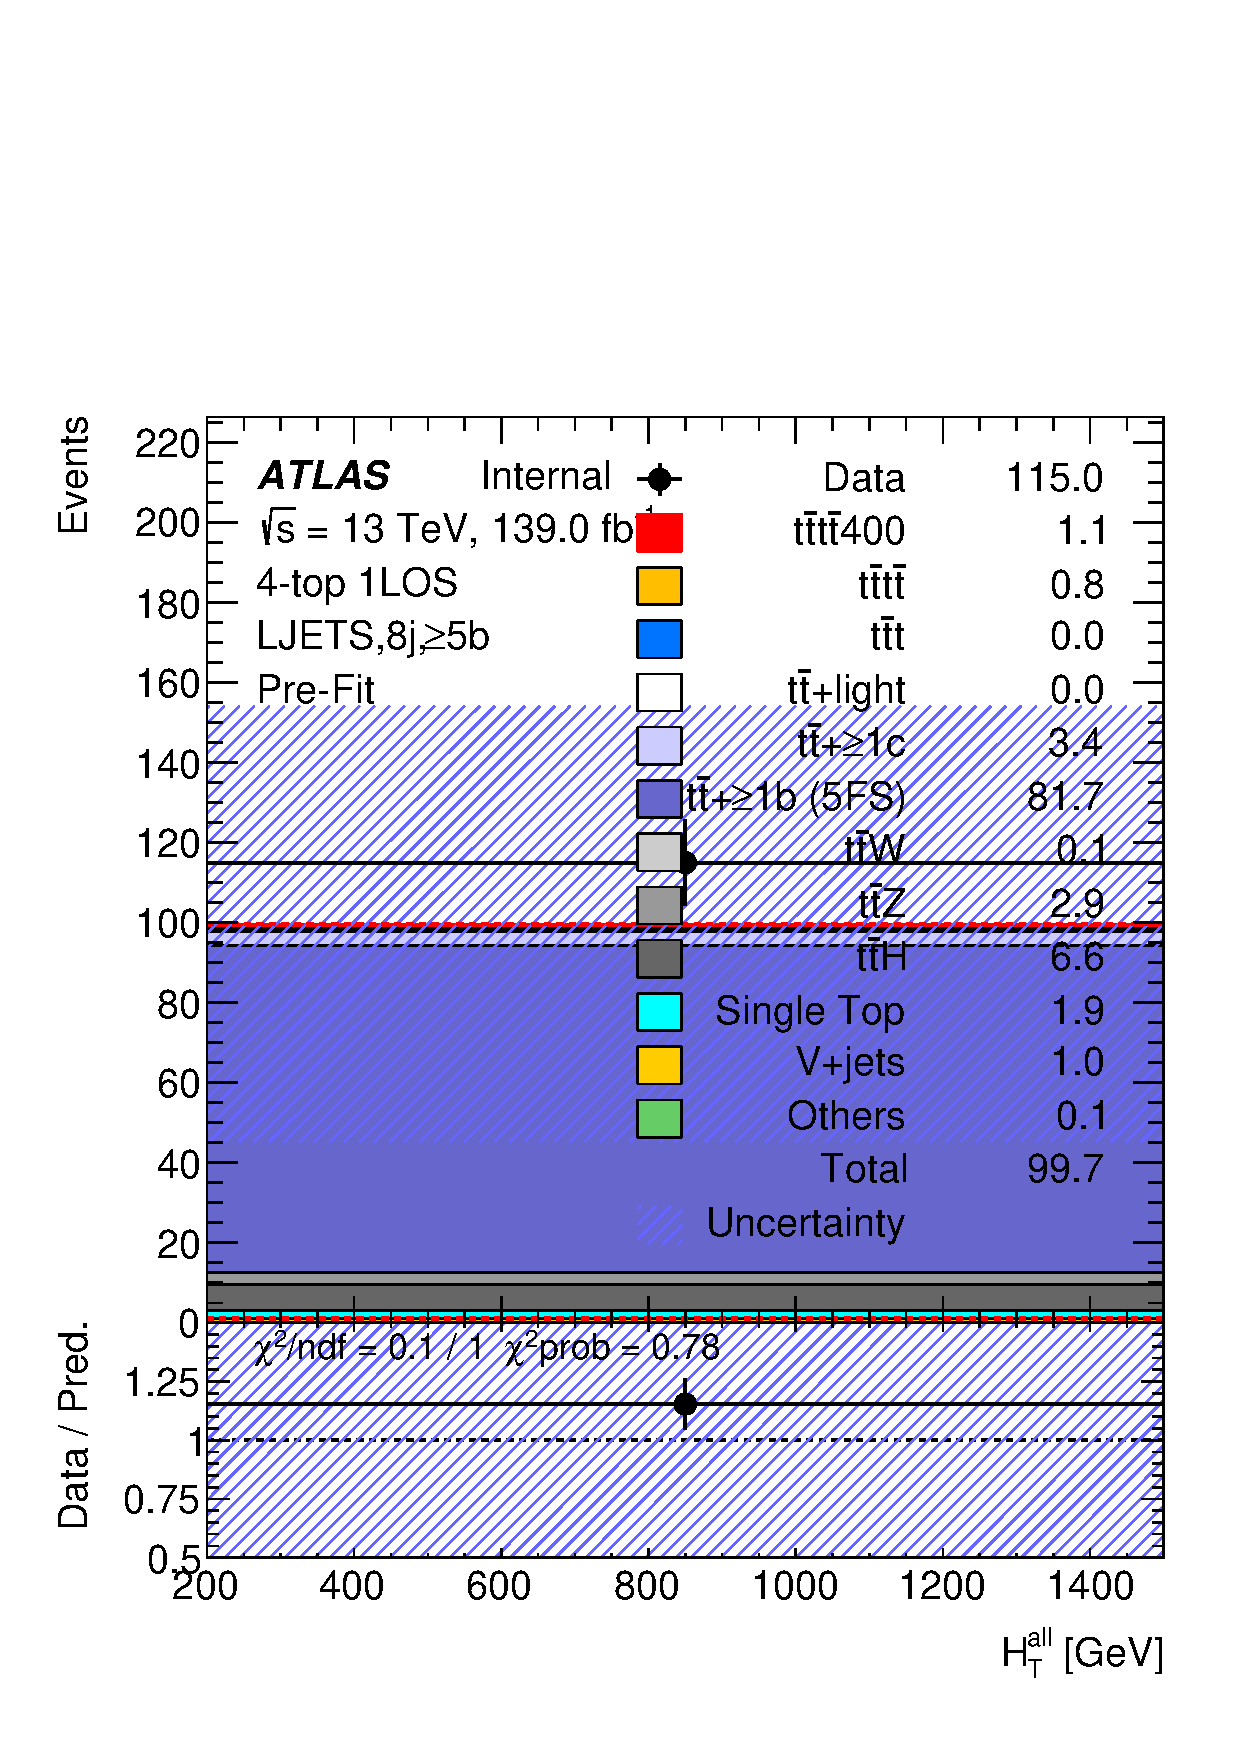
\includegraphics[width=0.23 \textwidth]{figures/fits/GNN/400/1L/data_unblindedSplusB/Plots/ljets_8jge5b.pdf}\\

        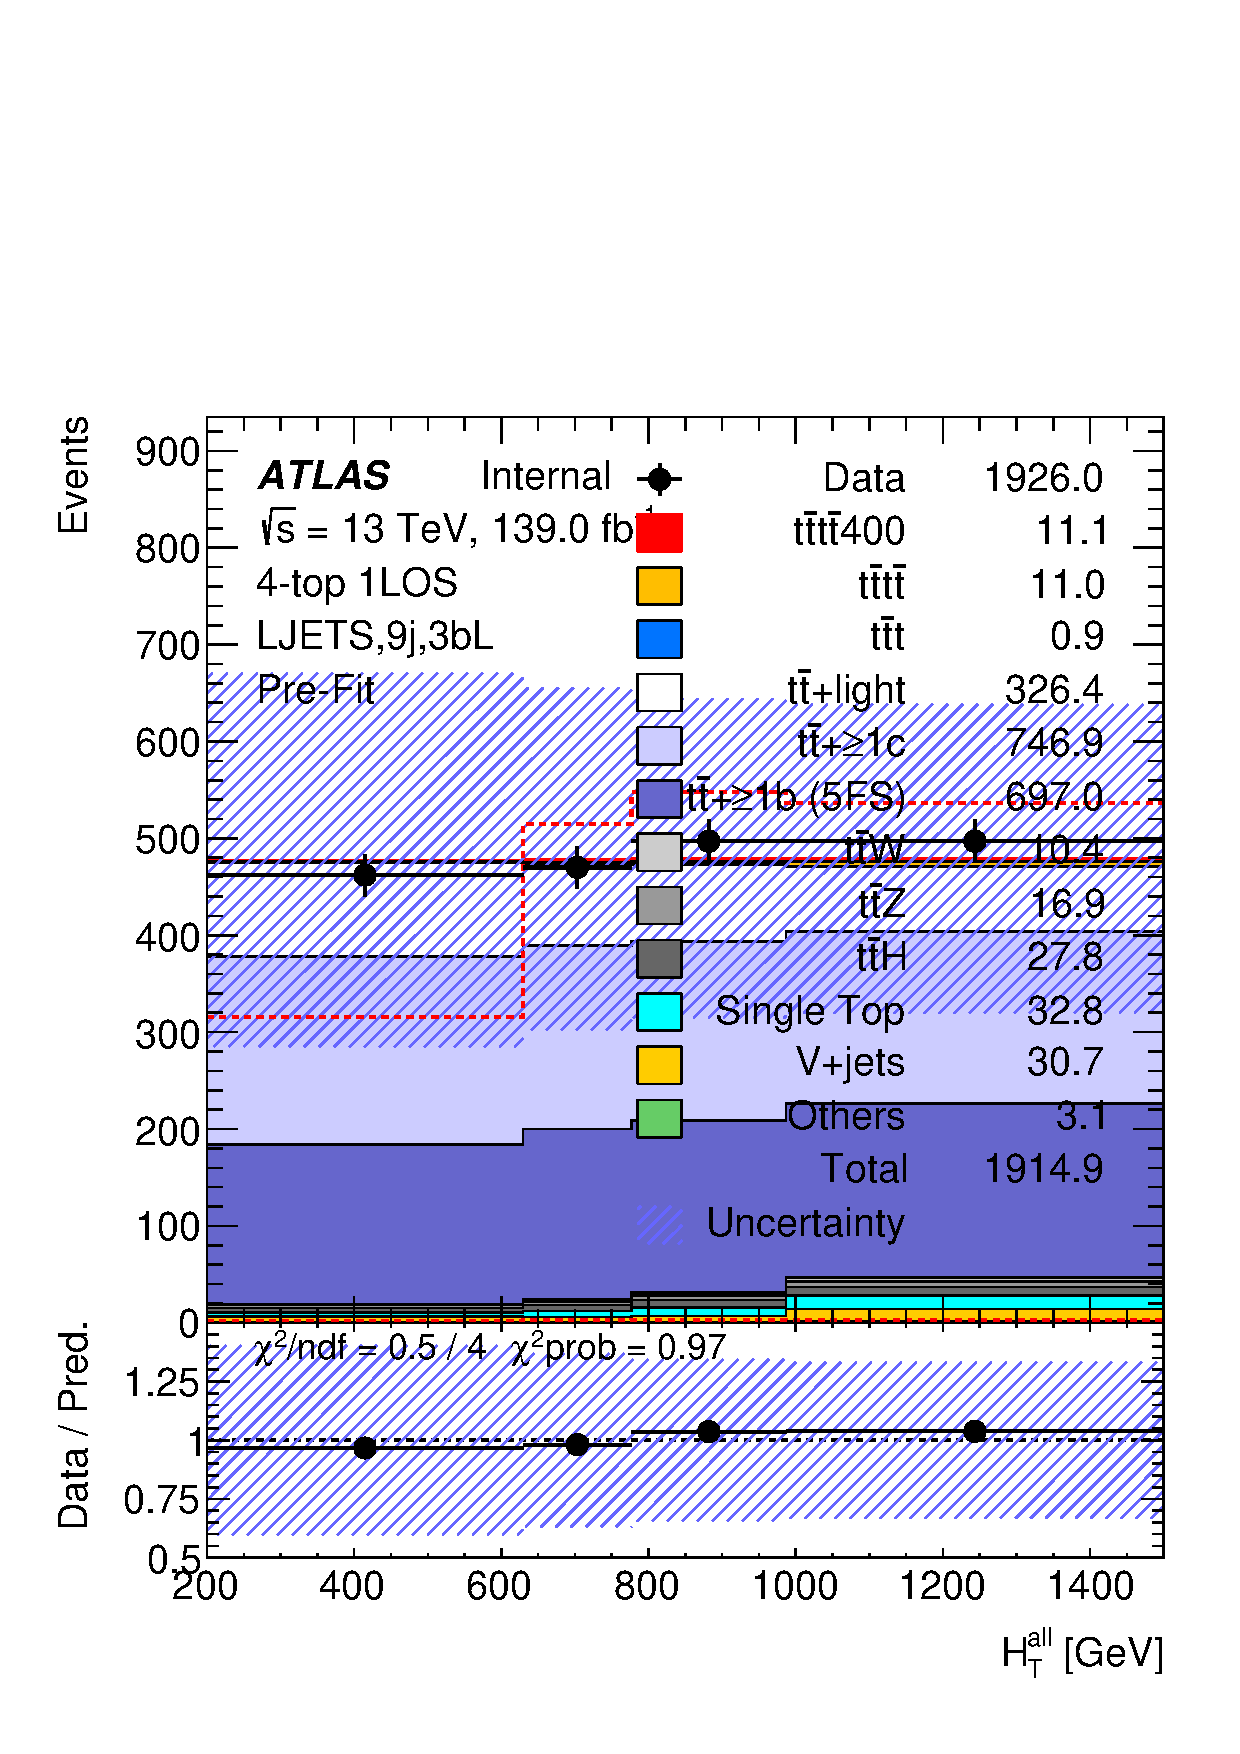
\includegraphics[width=0.23 \textwidth]{figures/fits/GNN/400/1L/data_unblindedSplusB/Plots/ljets_9j3bL.pdf} &
        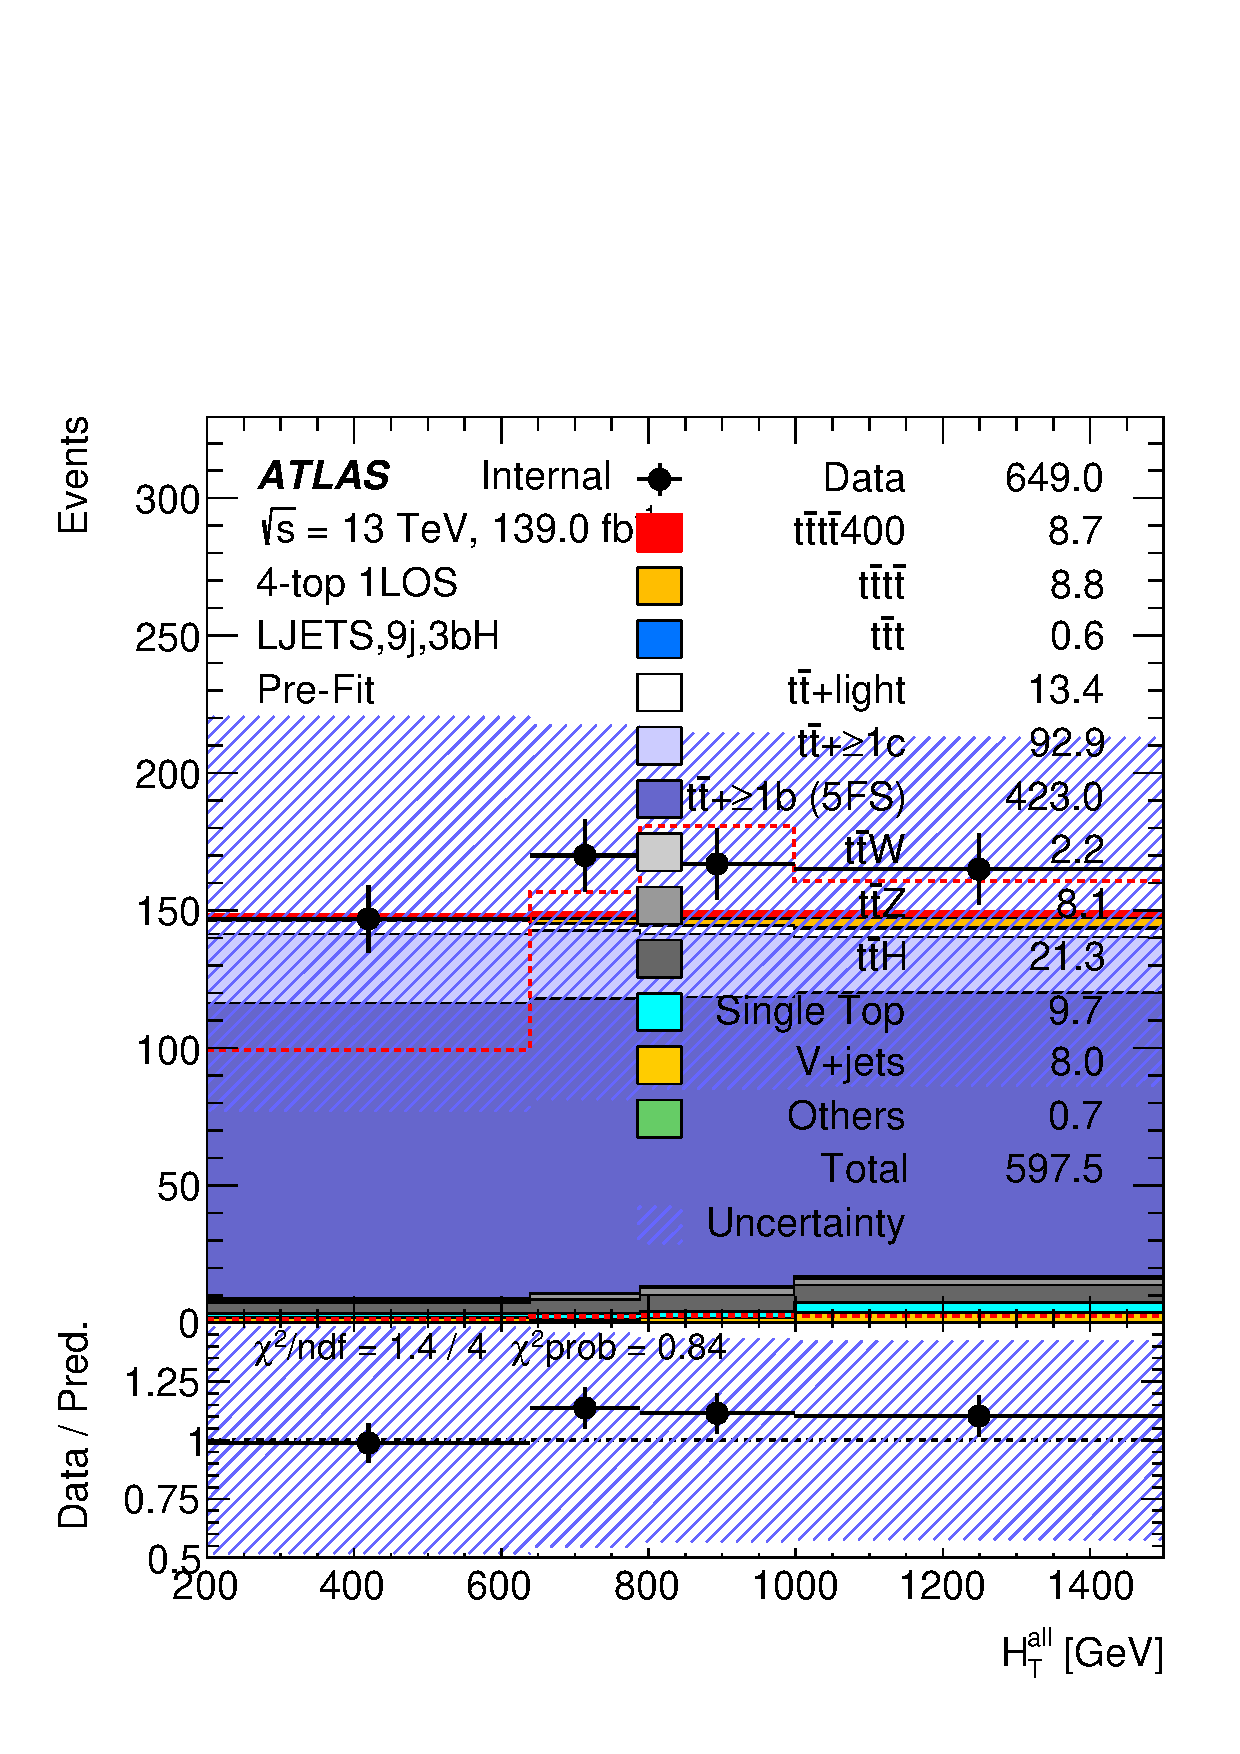
\includegraphics[width=0.23 \textwidth]{figures/fits/GNN/400/1L/data_unblindedSplusB/Plots/ljets_9j3bH.pdf} &
        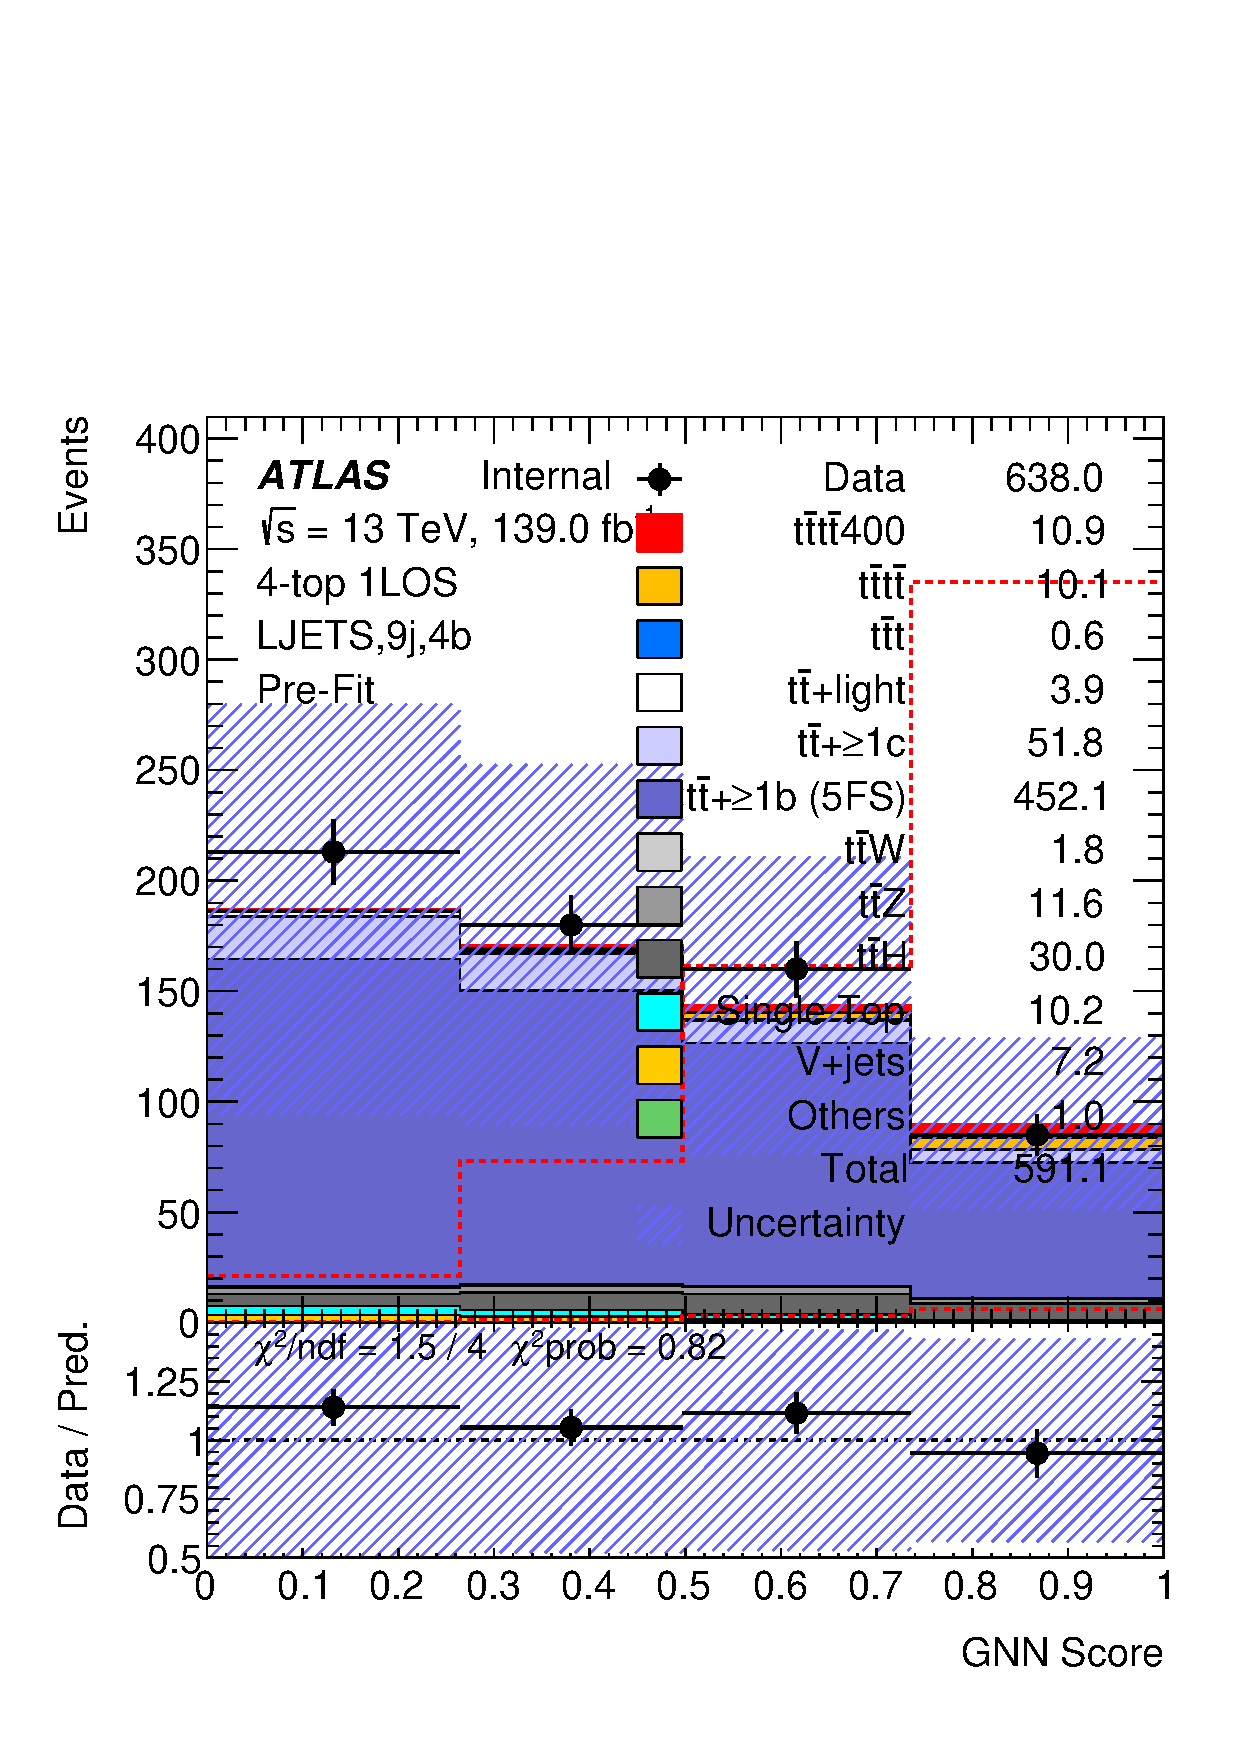
\includegraphics[width=0.23 \textwidth]{figures/fits/GNN/400/1L/data_unblindedSplusB/Plots/ljets_9j4b.pdf} &
        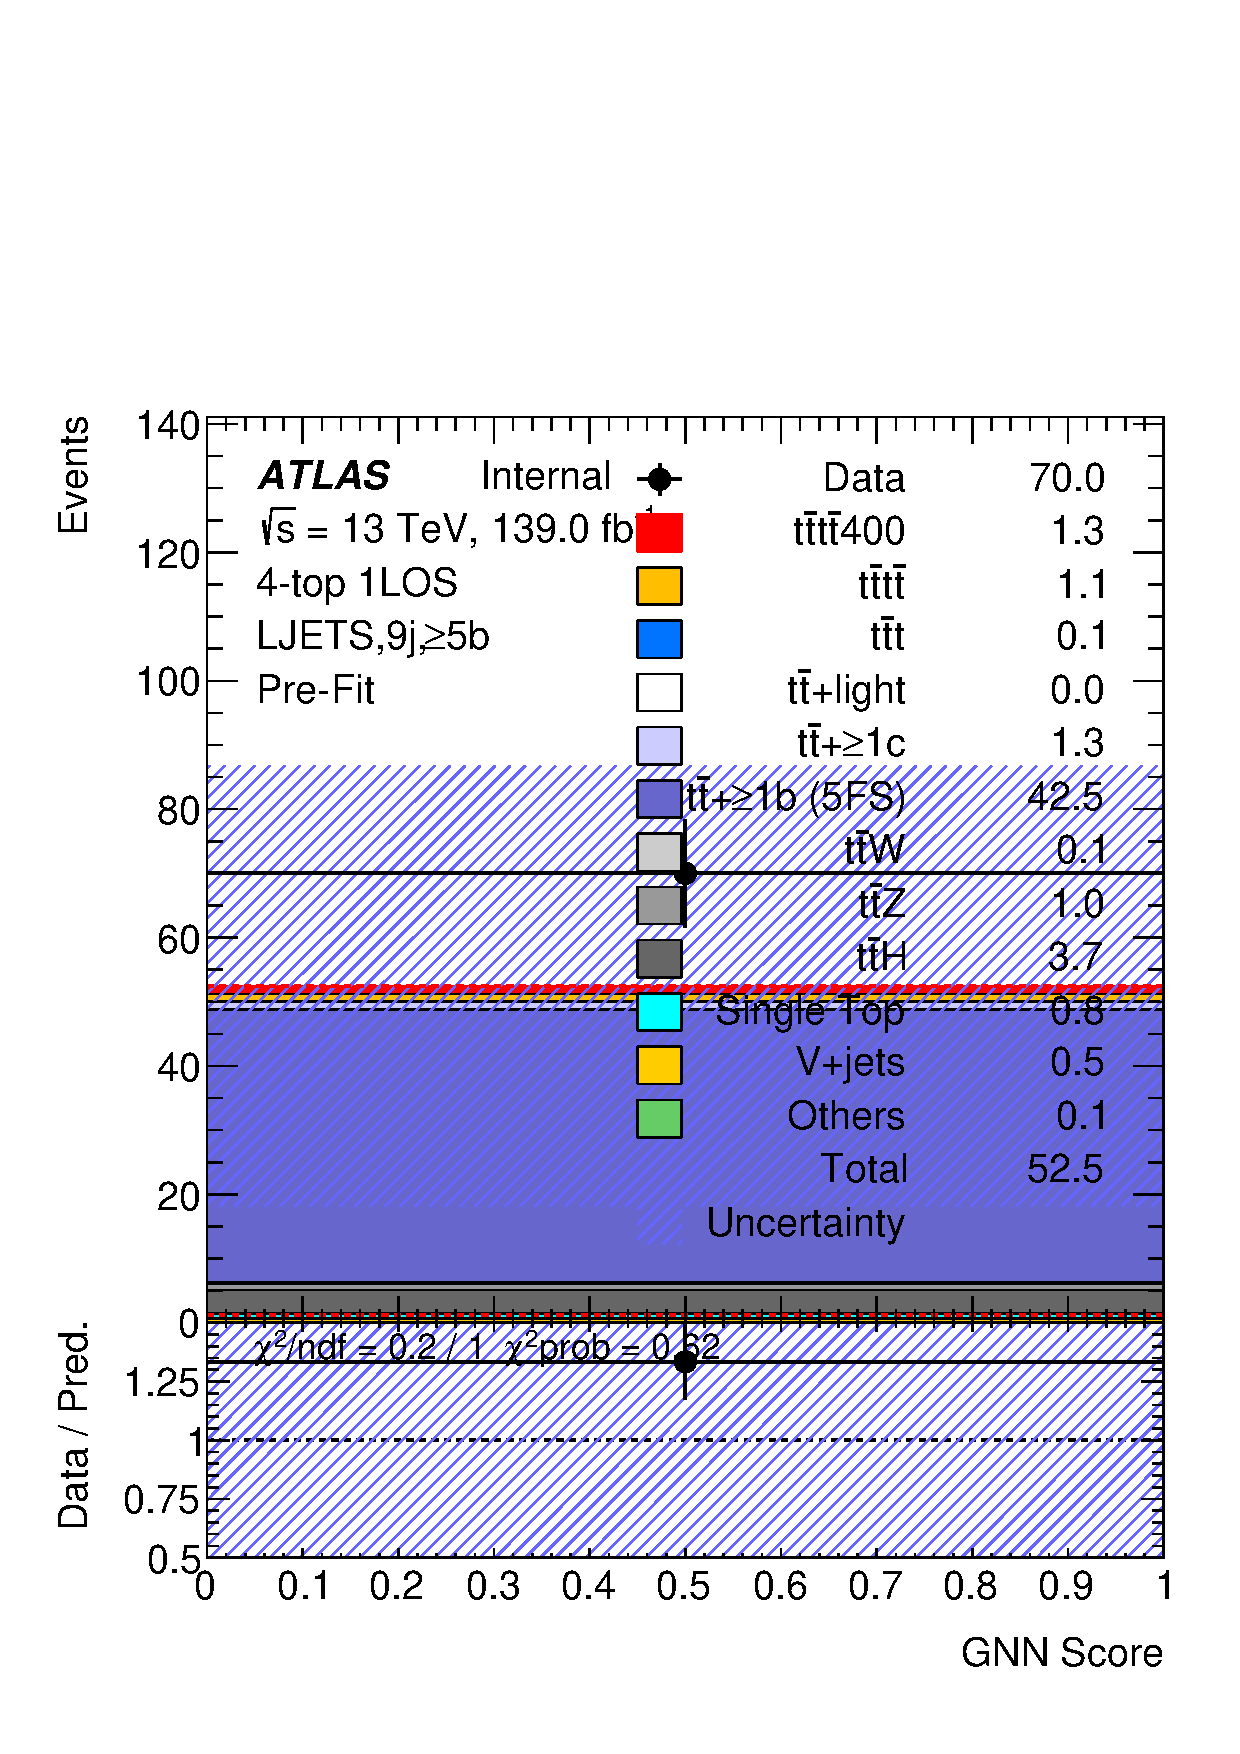
\includegraphics[width=0.23 \textwidth]{figures/fits/GNN/400/1L/data_unblindedSplusB/Plots/ljets_9jge5b.pdf} \\

        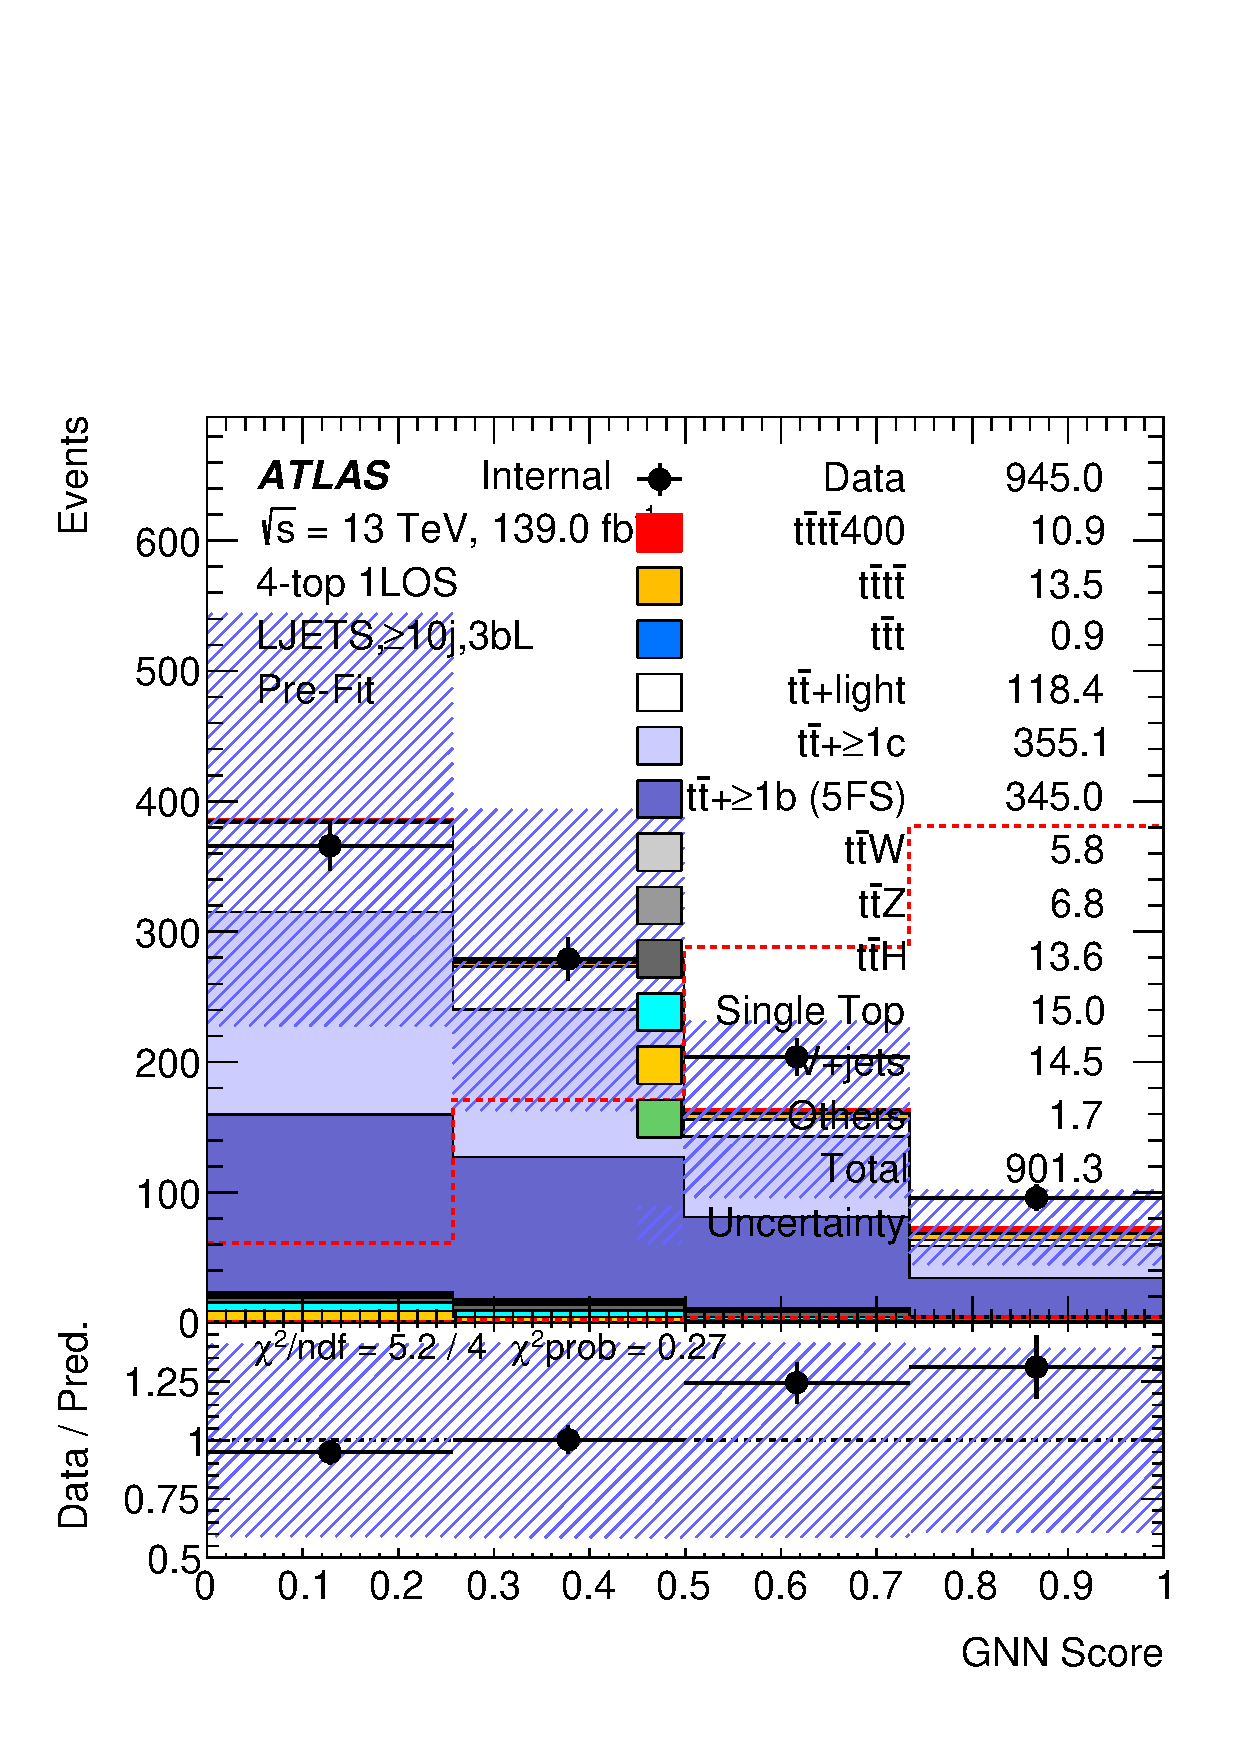
\includegraphics[width=0.23 \textwidth]{figures/fits/GNN/400/1L/data_unblindedSplusB/Plots/ljets_ge10j3bL.pdf} &
        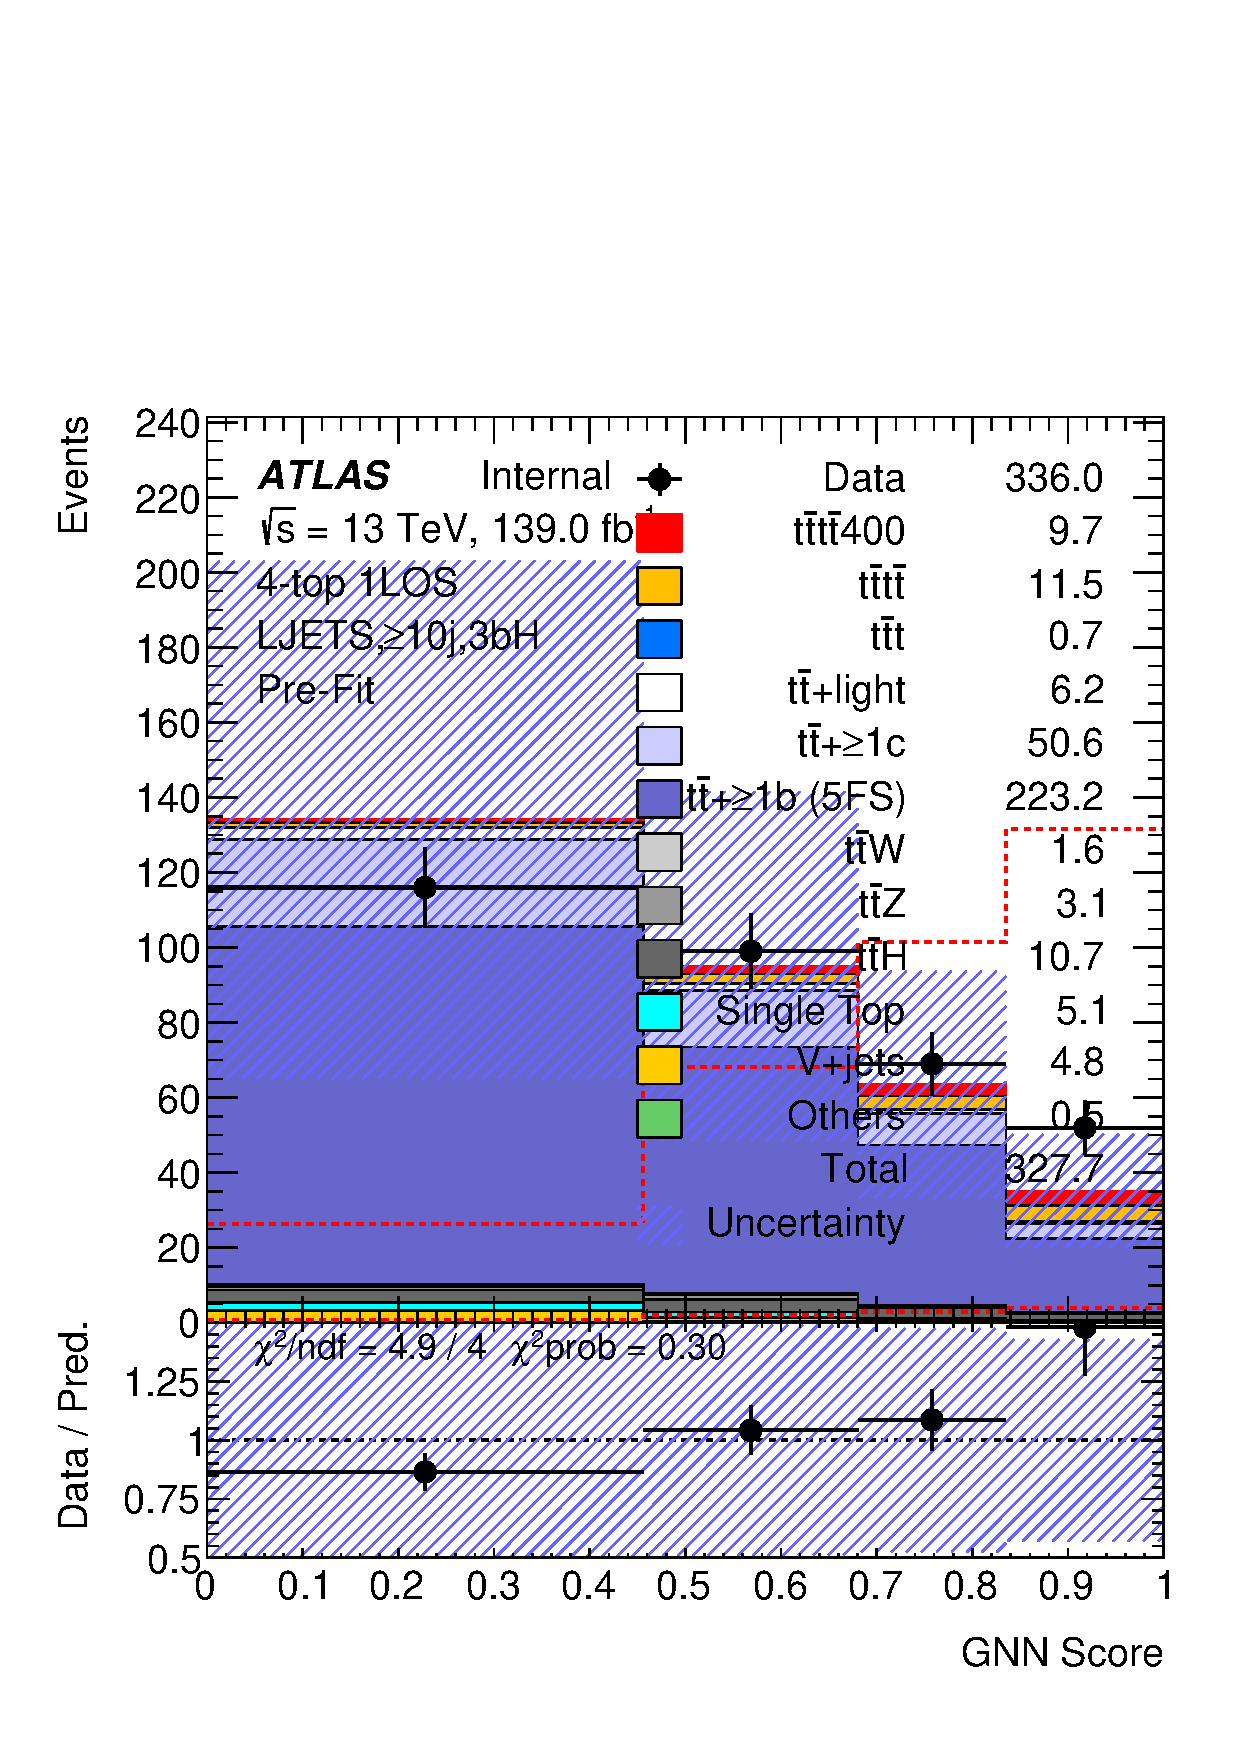
\includegraphics[width=0.23 \textwidth]{figures/fits/GNN/400/1L/data_unblindedSplusB/Plots/ljets_ge10j3bH.pdf} &
        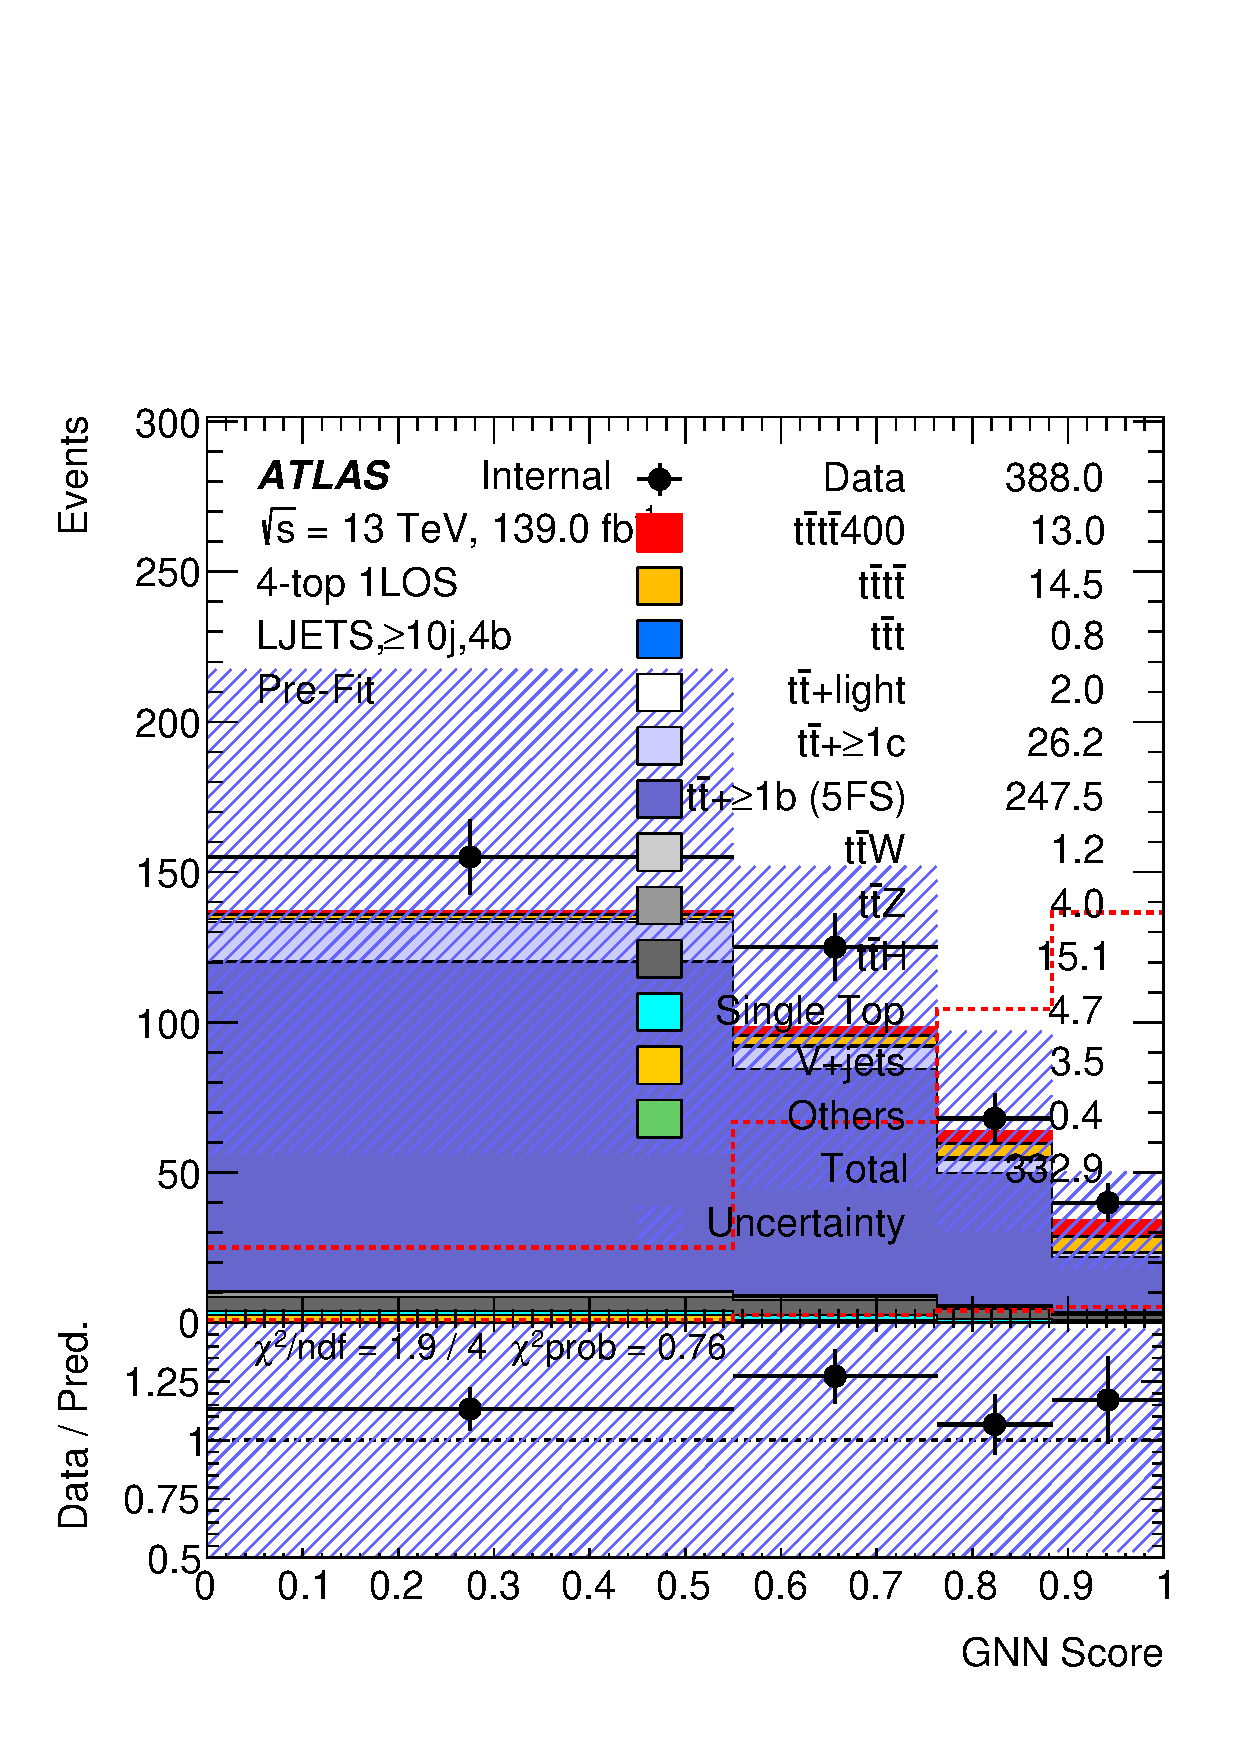
\includegraphics[width=0.23 \textwidth]{figures/fits/GNN/400/1L/data_unblindedSplusB/Plots/ljets_ge10j4b.pdf} &
        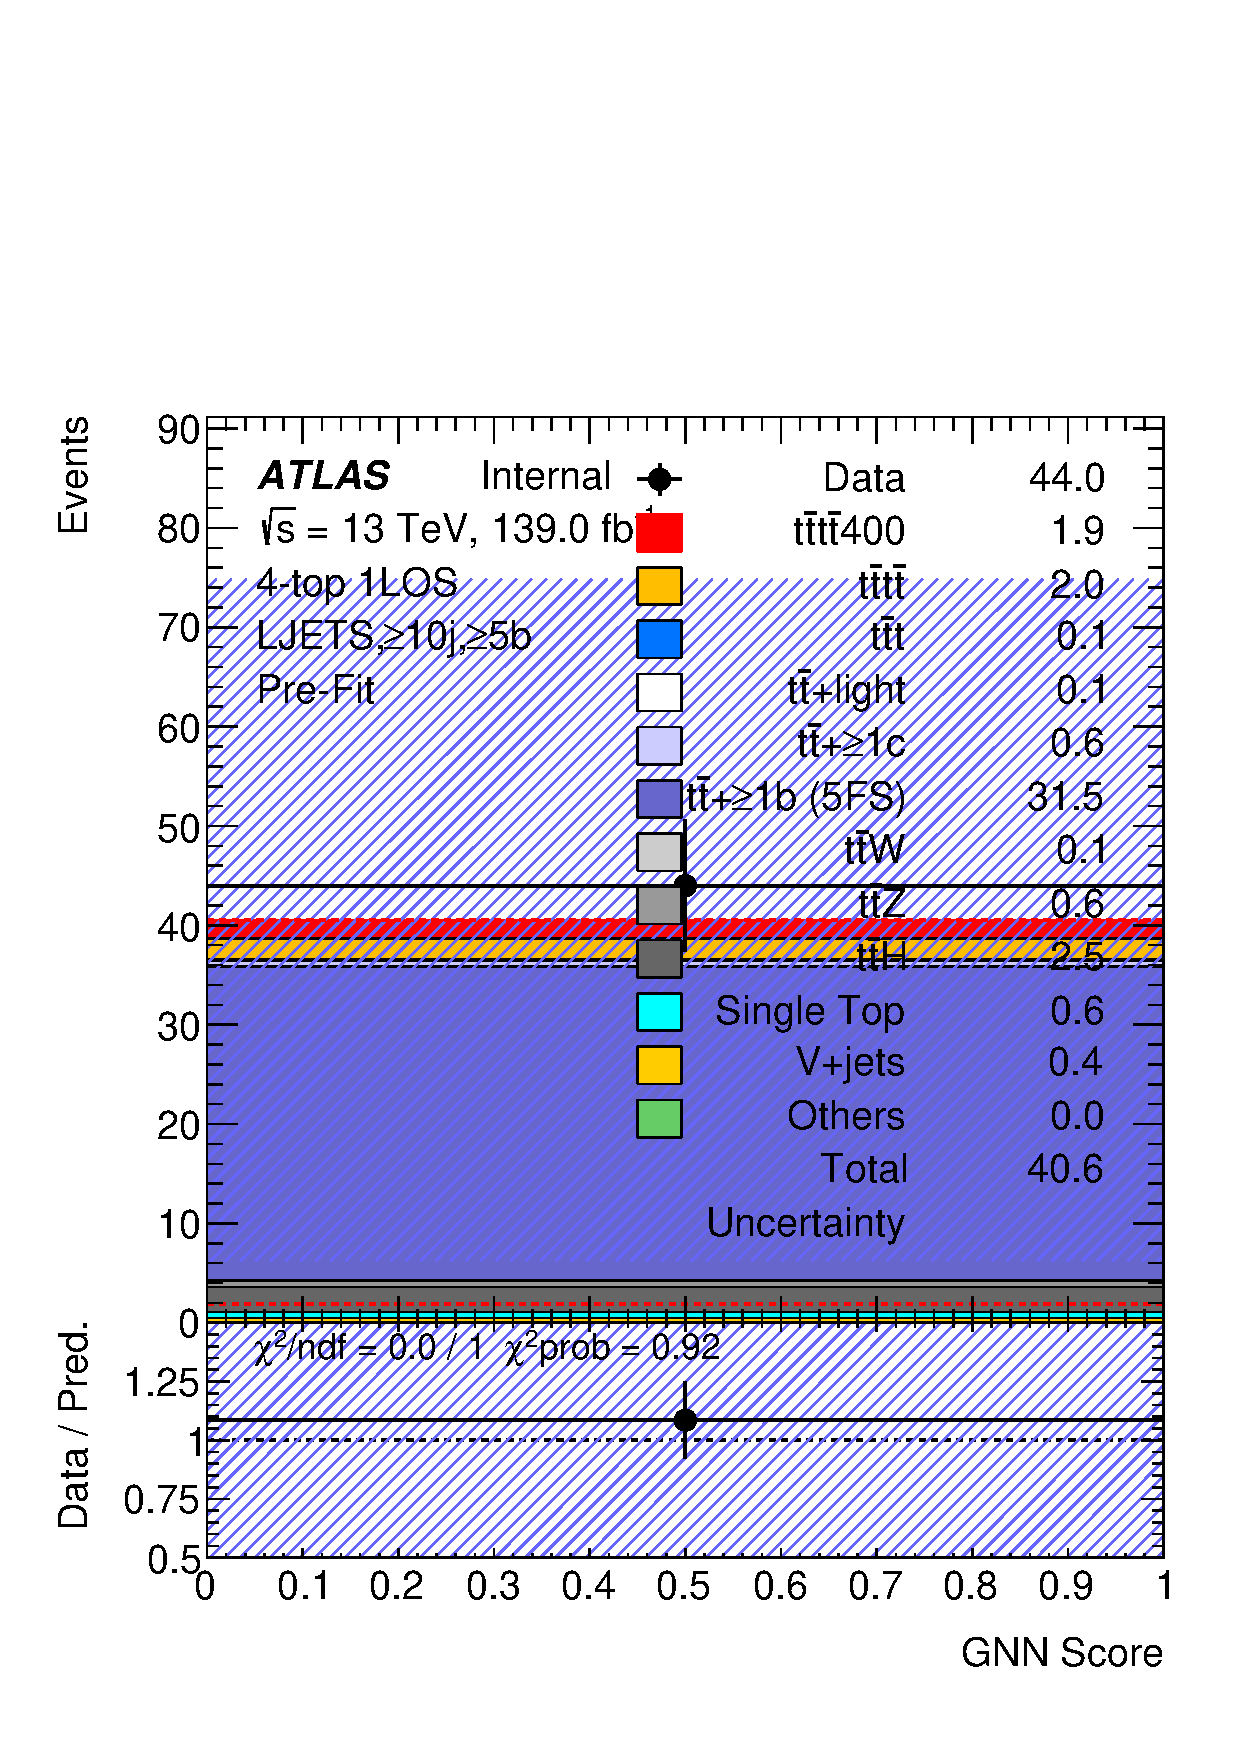
\includegraphics[width=0.23 \textwidth]{figures/fits/GNN/400/1L/data_unblindedSplusB/Plots/ljets_ge10jge5b.pdf} \\
        \end{tabular}
        \caption{\label{fig:Prefit_Yields_1L}Pre-fit distributions for 1L channel associated with different signal and background samples, compared with data yields. In general, MC samples and data have good agreement. The signal sample is normalised to a cross-section of 12 fb.}
\end{center}
\end{figure}

\begin{figure}[htbp!]
        \begin{center} \setlength{\tabcolsep}{2.5pt}\footnotesize
        \begin{tabular}{ccc}
        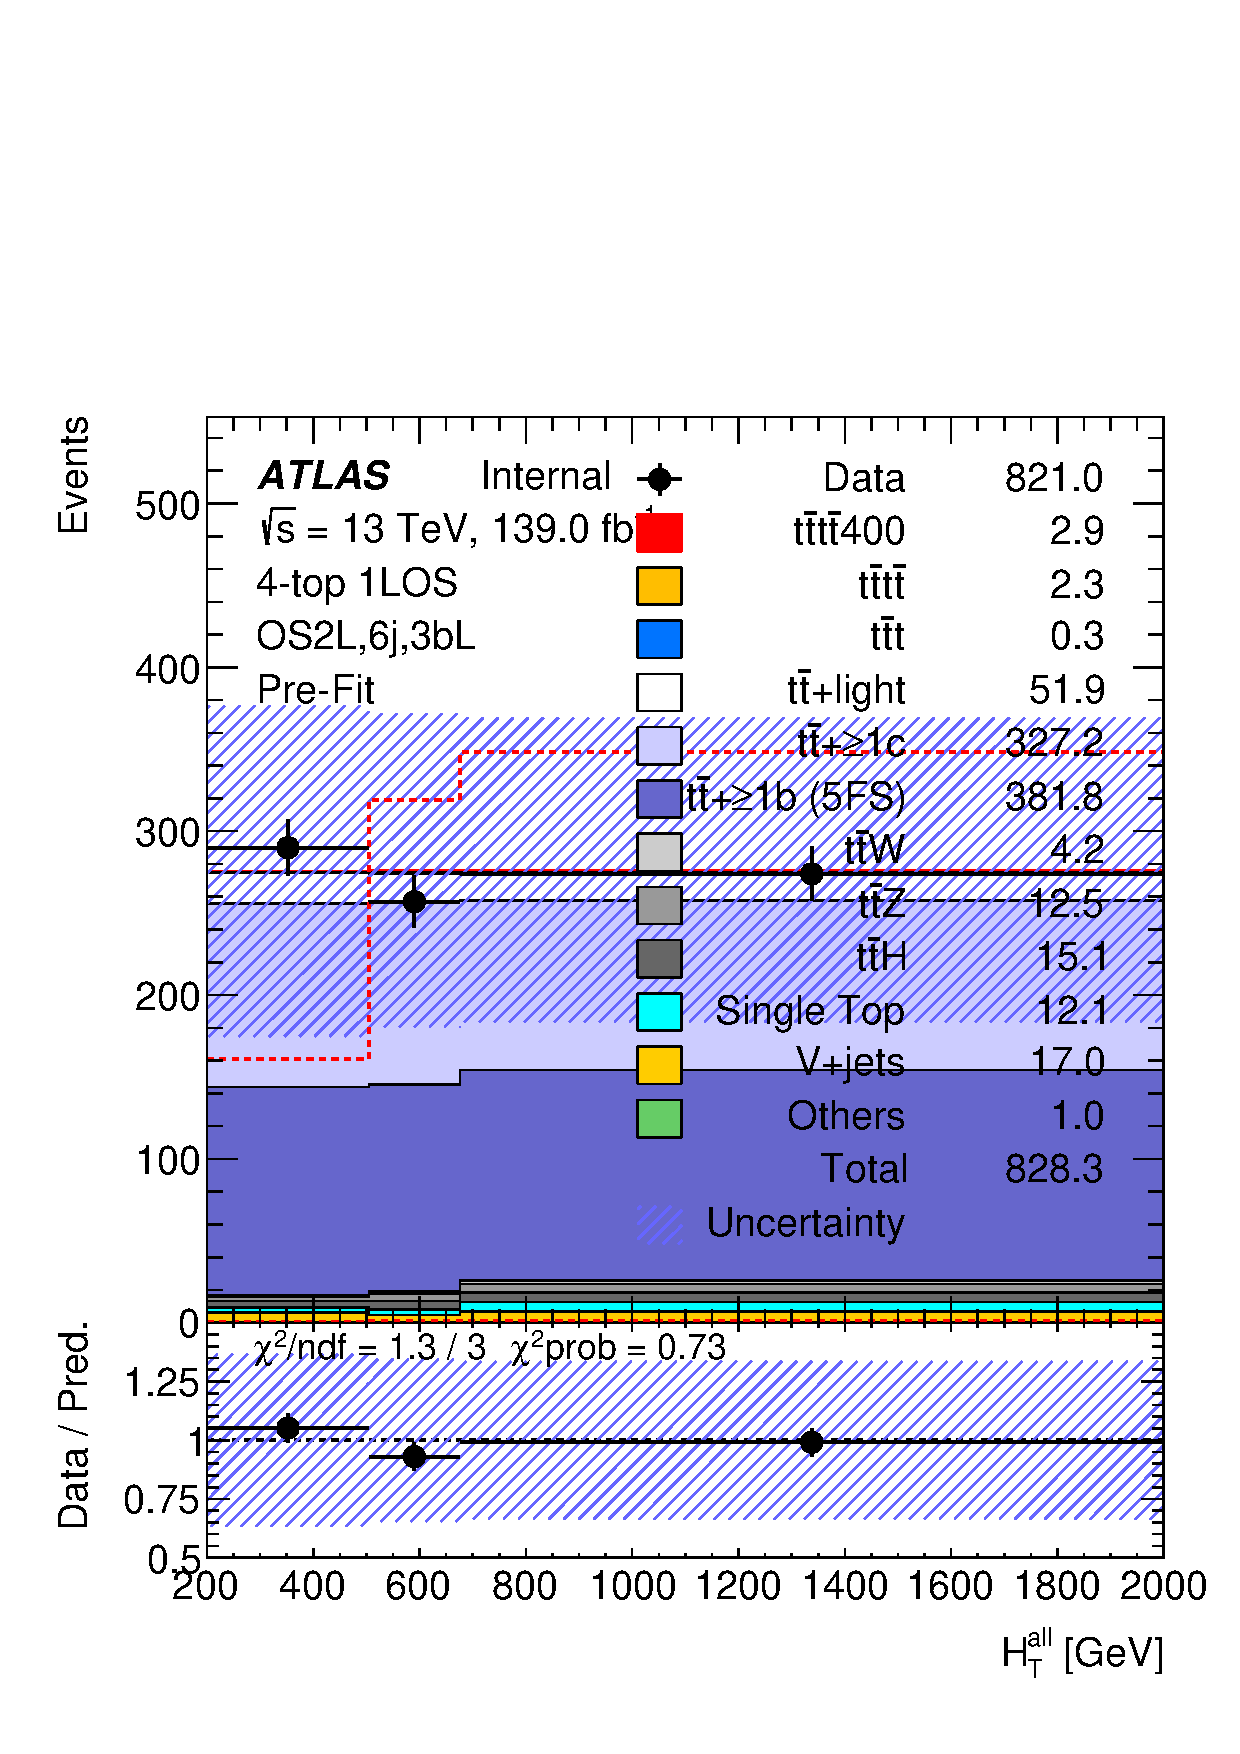
\includegraphics[width=0.31 \textwidth]{figures/fits/GNN/400/2L/data_unblindedSplusB/Plots/os2l_6j3bL.pdf} &
        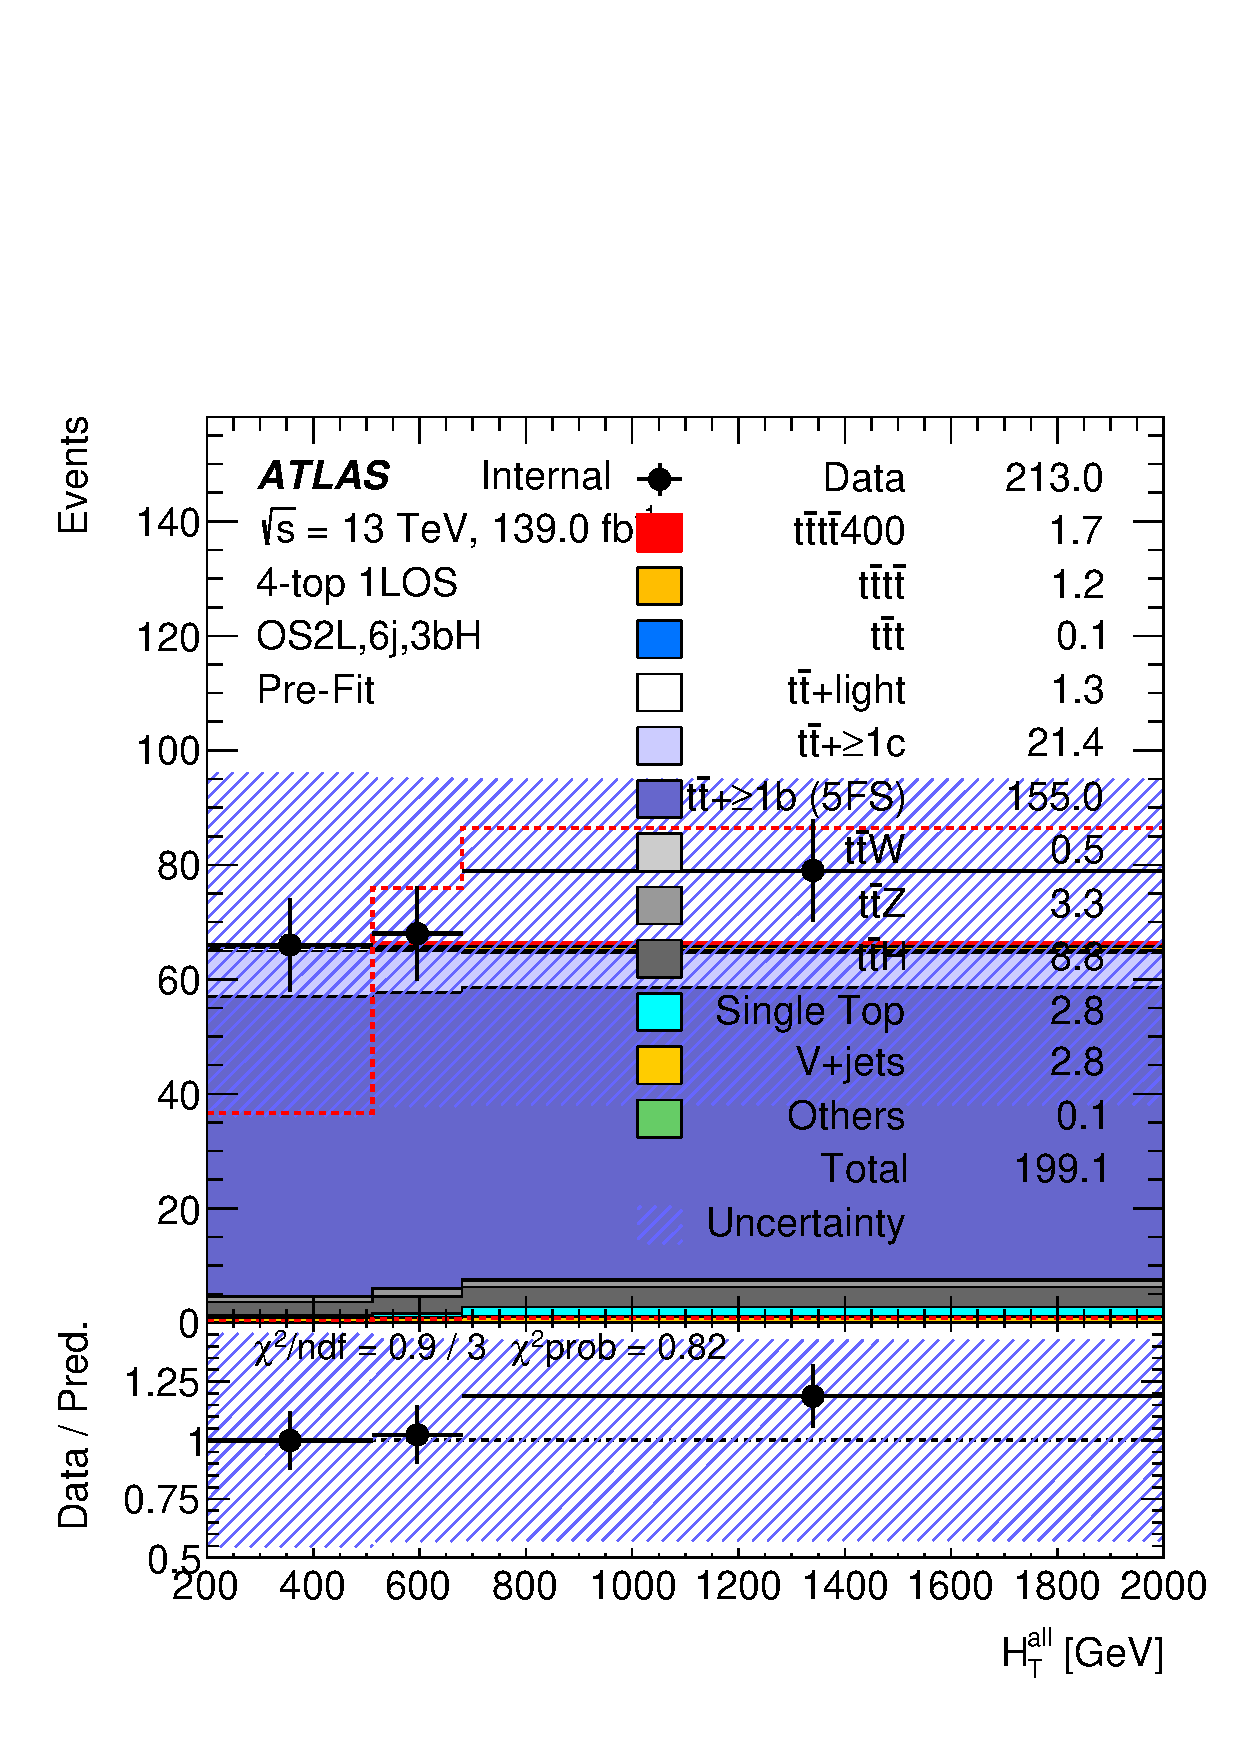
\includegraphics[width=0.31 \textwidth]{figures/fits/GNN/400/2L/data_unblindedSplusB/Plots/os2l_6j3bH.pdf} &
        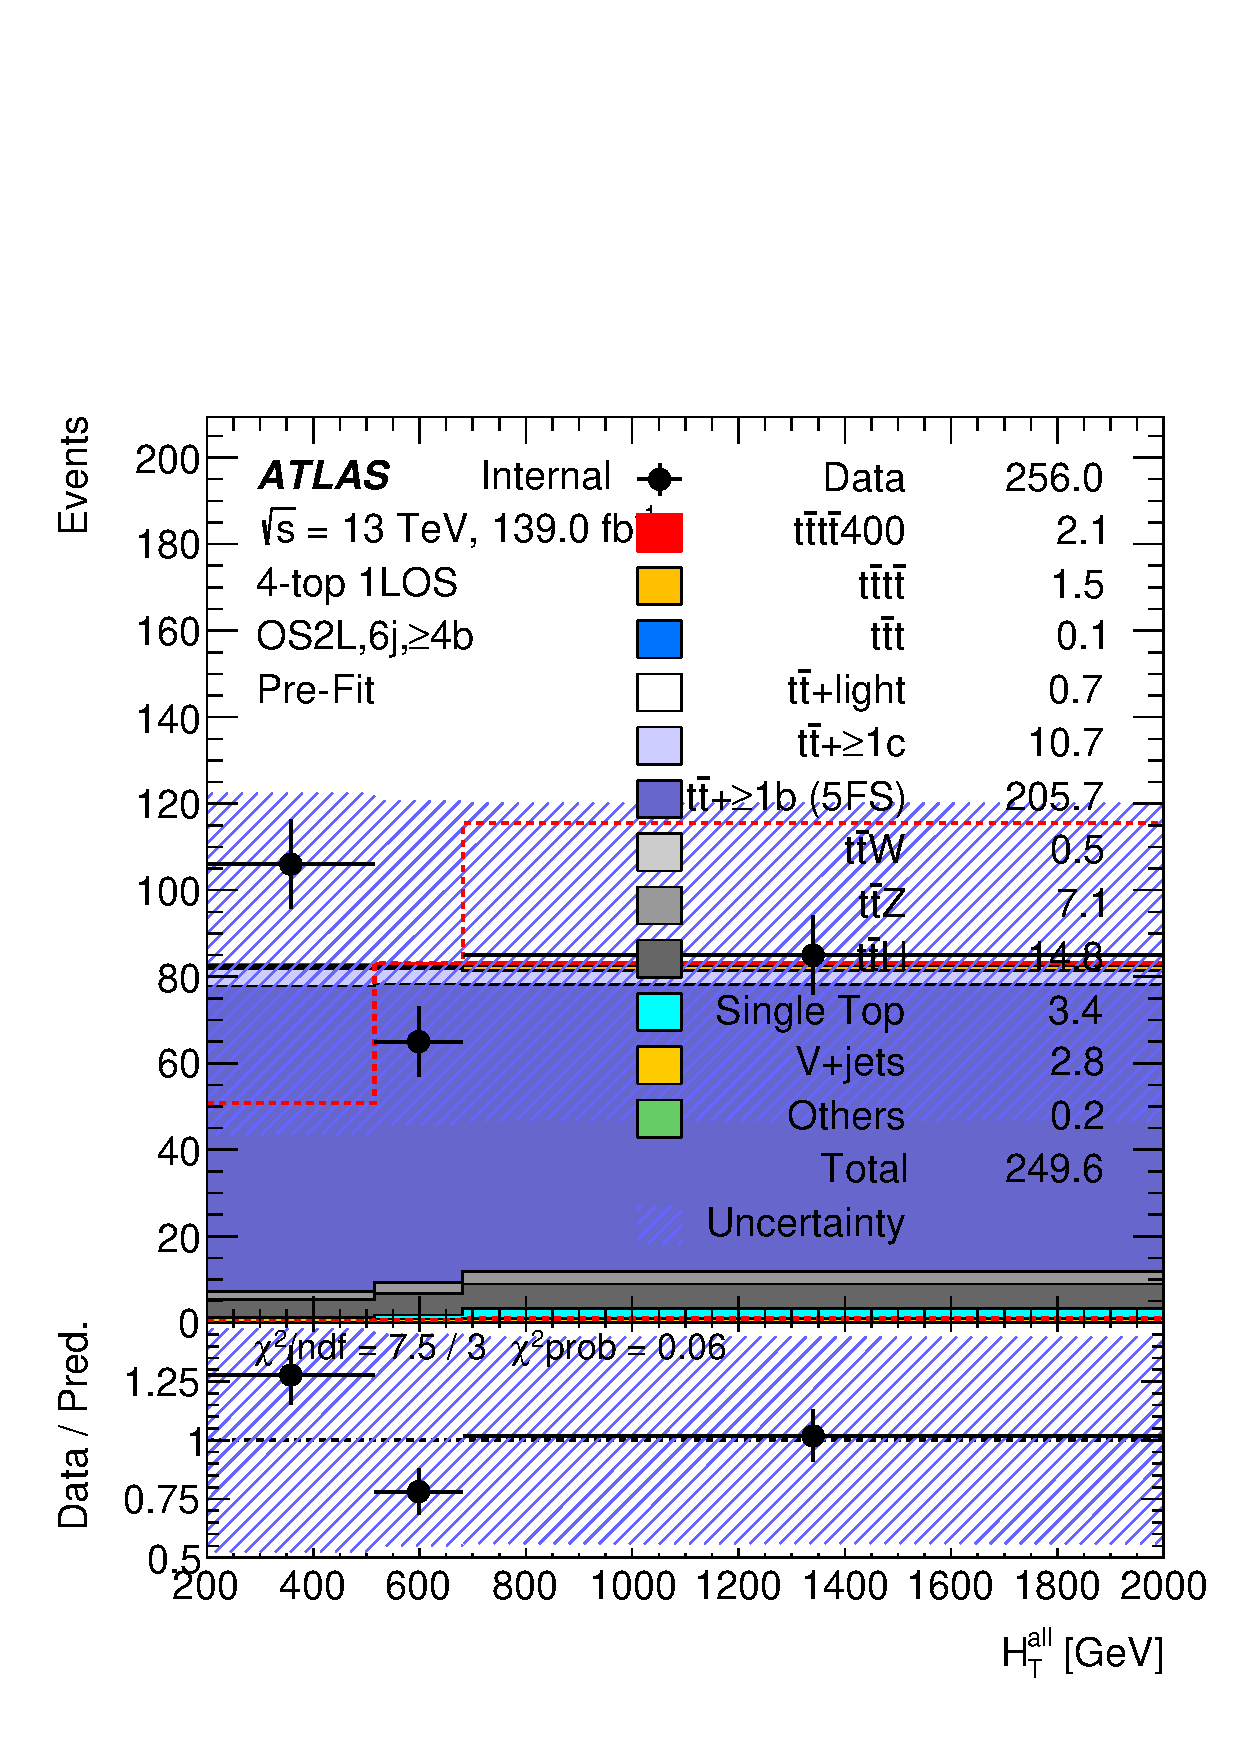
\includegraphics[width=0.31 \textwidth]{figures/fits/GNN/400/2L/data_unblindedSplusB/Plots/os2l_6jge4b.pdf} \\

        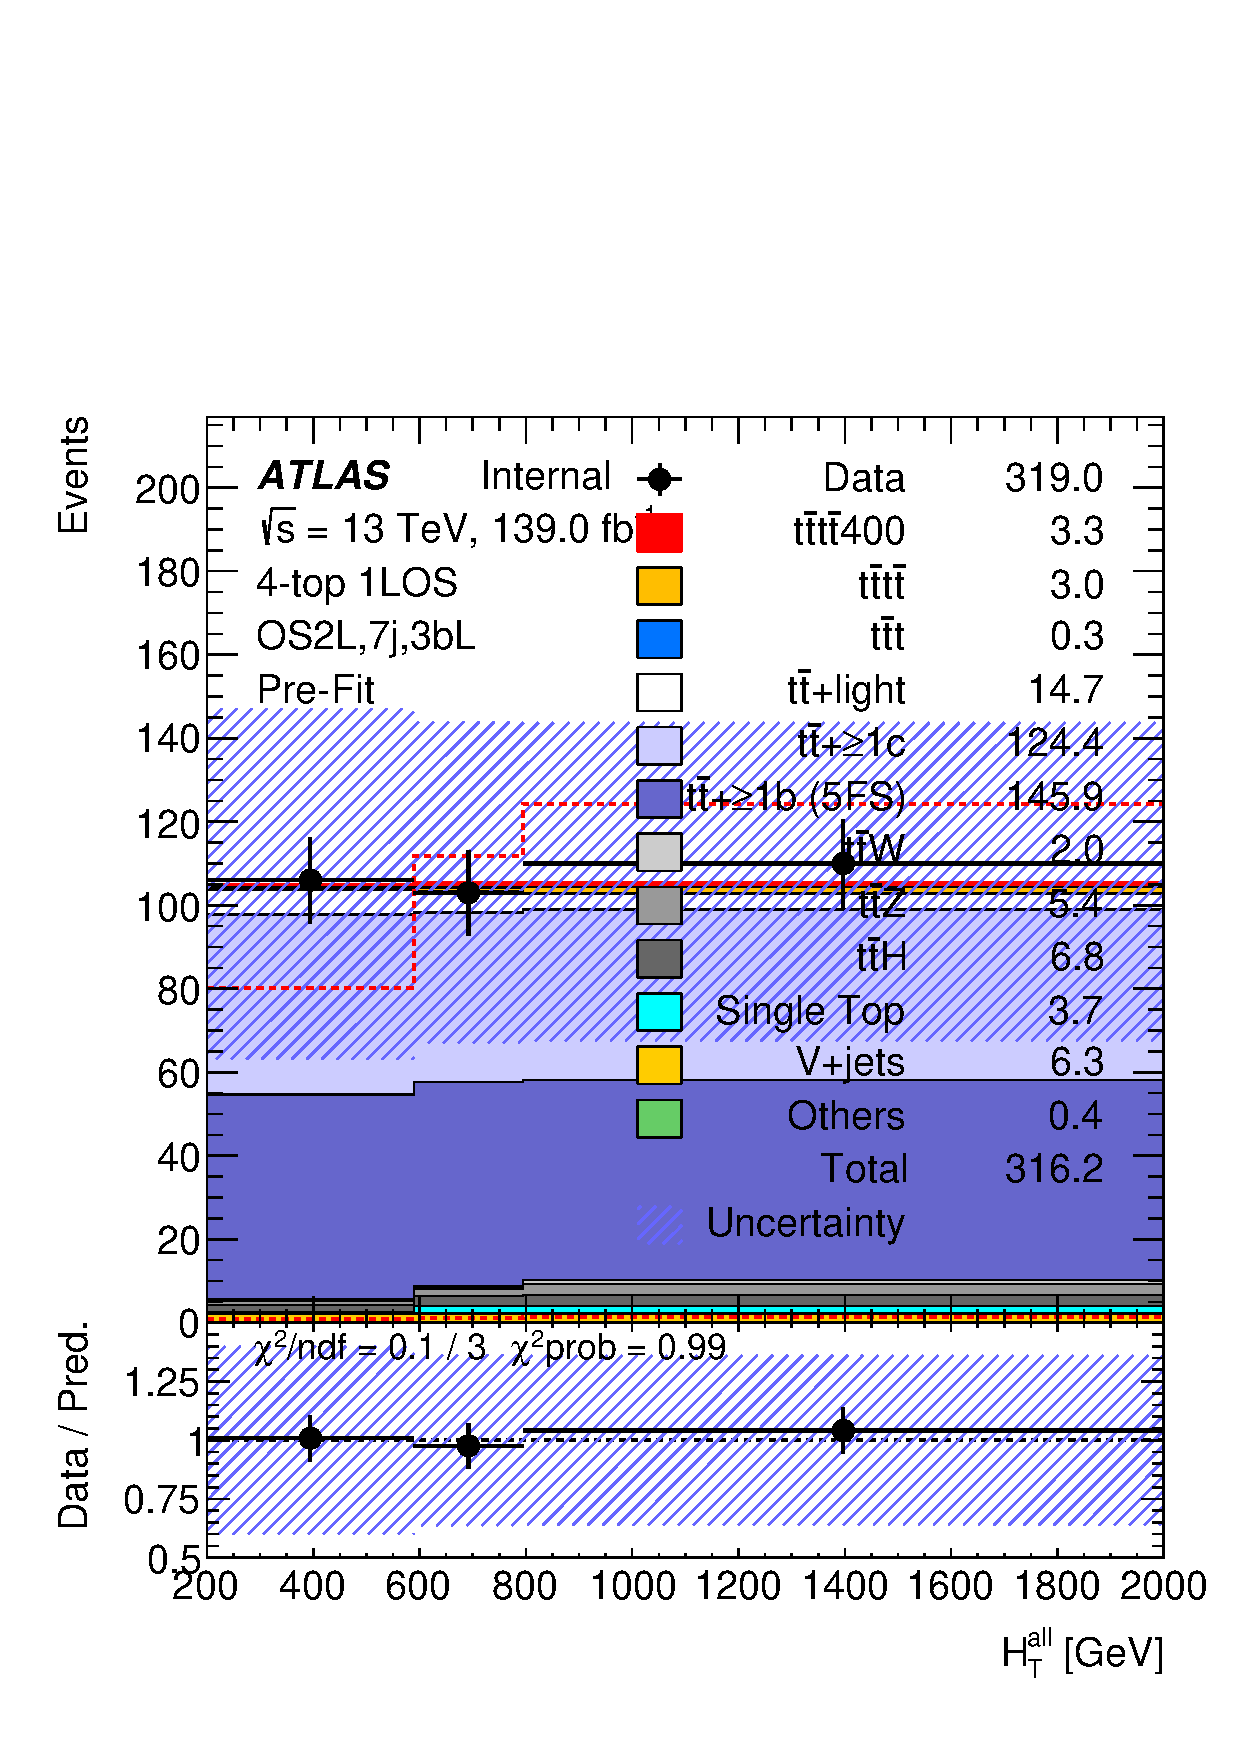
\includegraphics[width=0.31 \textwidth]{figures/fits/GNN/400/2L/data_unblindedSplusB/Plots/os2l_7j3bL.pdf} &
        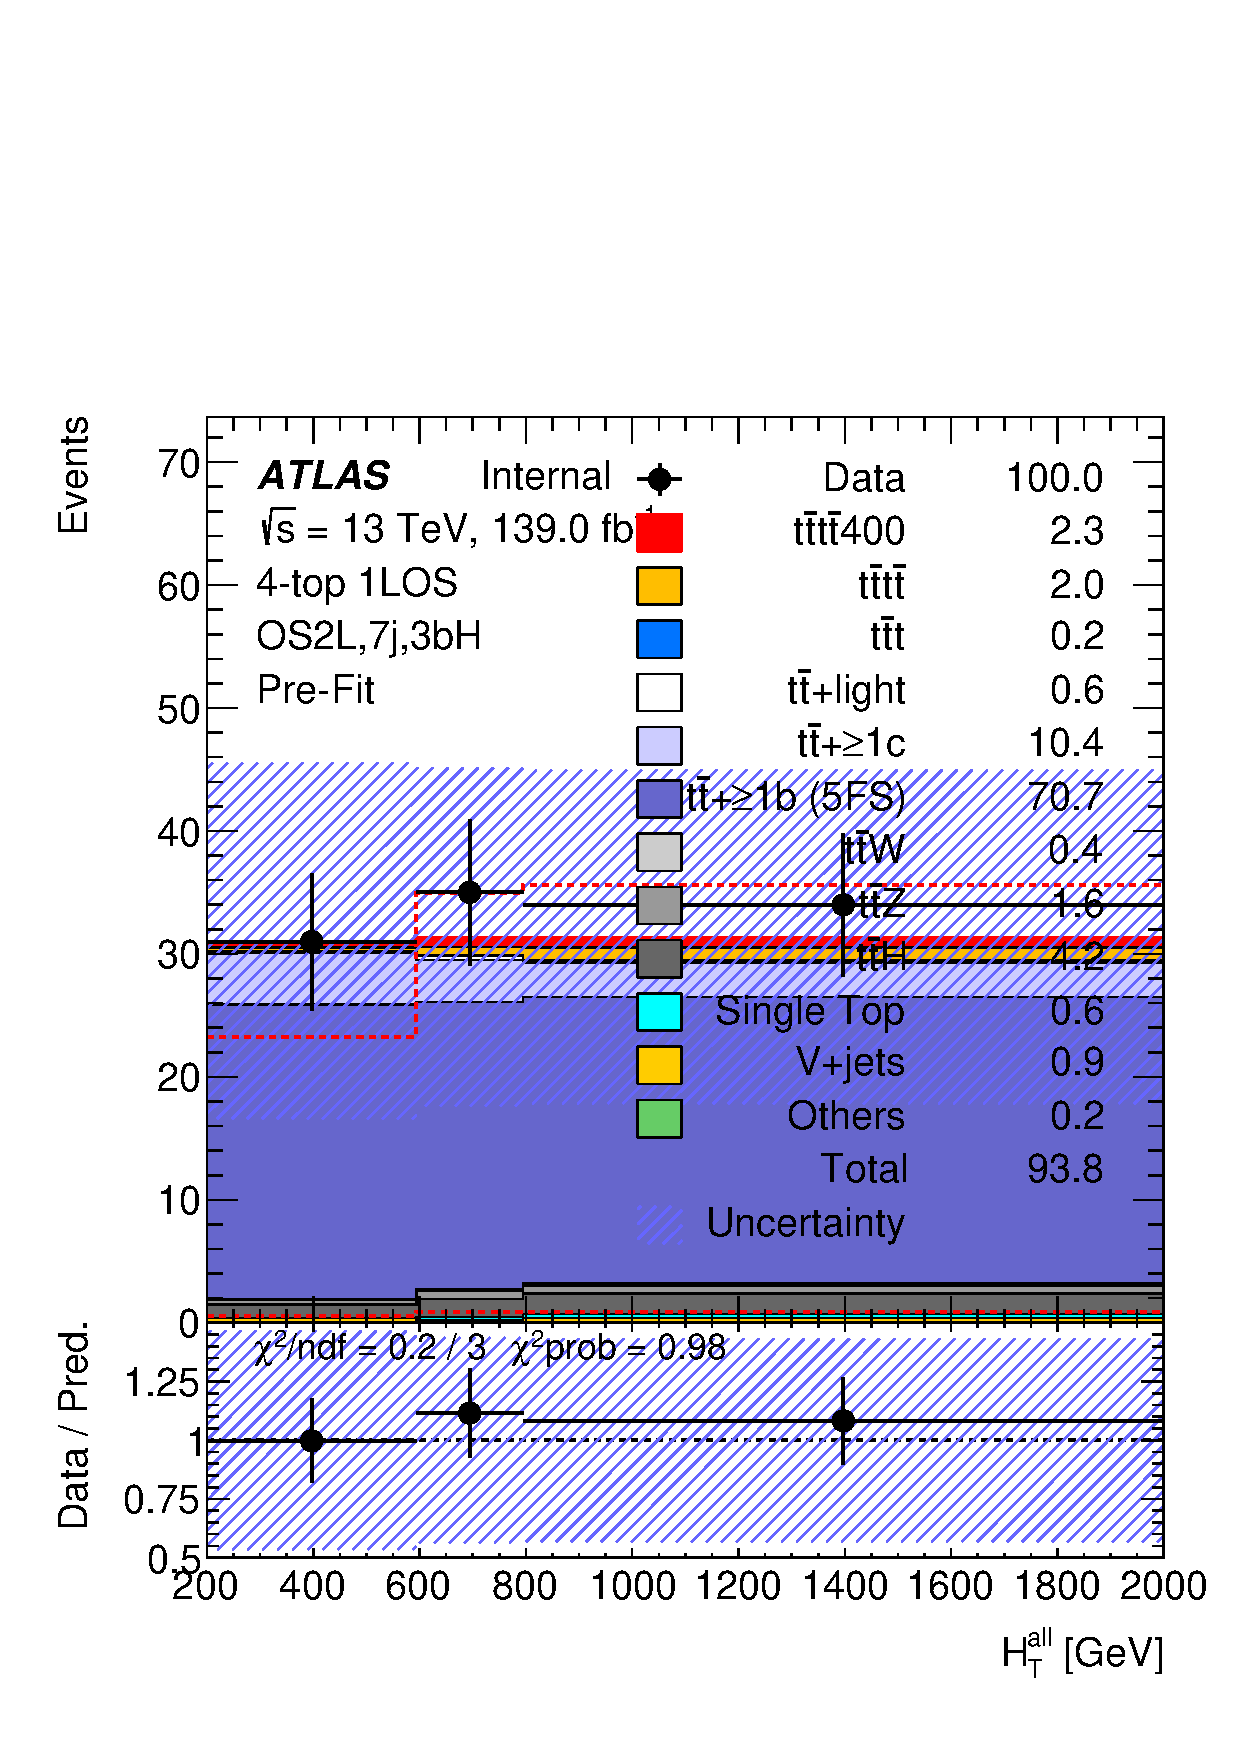
\includegraphics[width=0.31 \textwidth]{figures/fits/GNN/400/2L/data_unblindedSplusB/Plots/os2l_7j3bH.pdf} &
        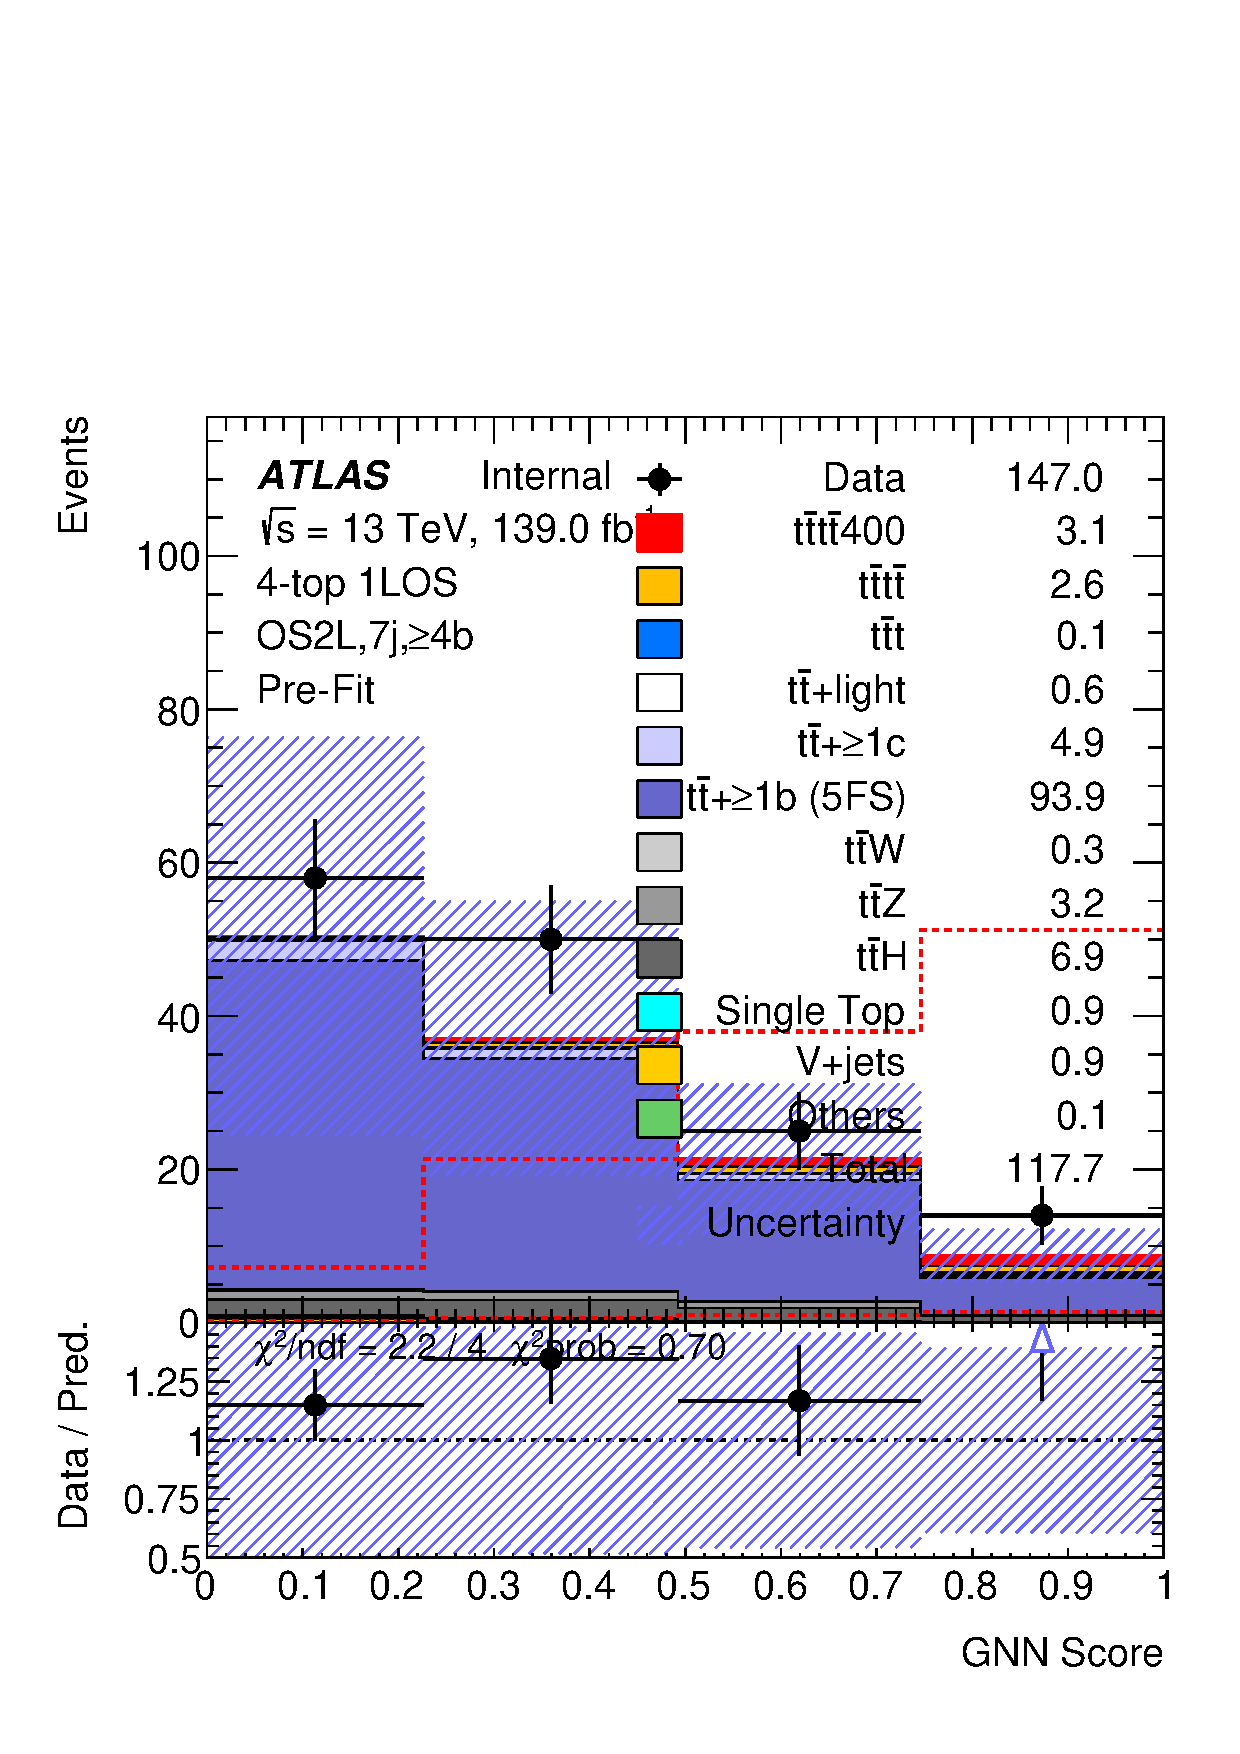
\includegraphics[width=0.31 \textwidth]{figures/fits/GNN/400/2L/data_unblindedSplusB/Plots/os2l_7jge4b.pdf} \\

        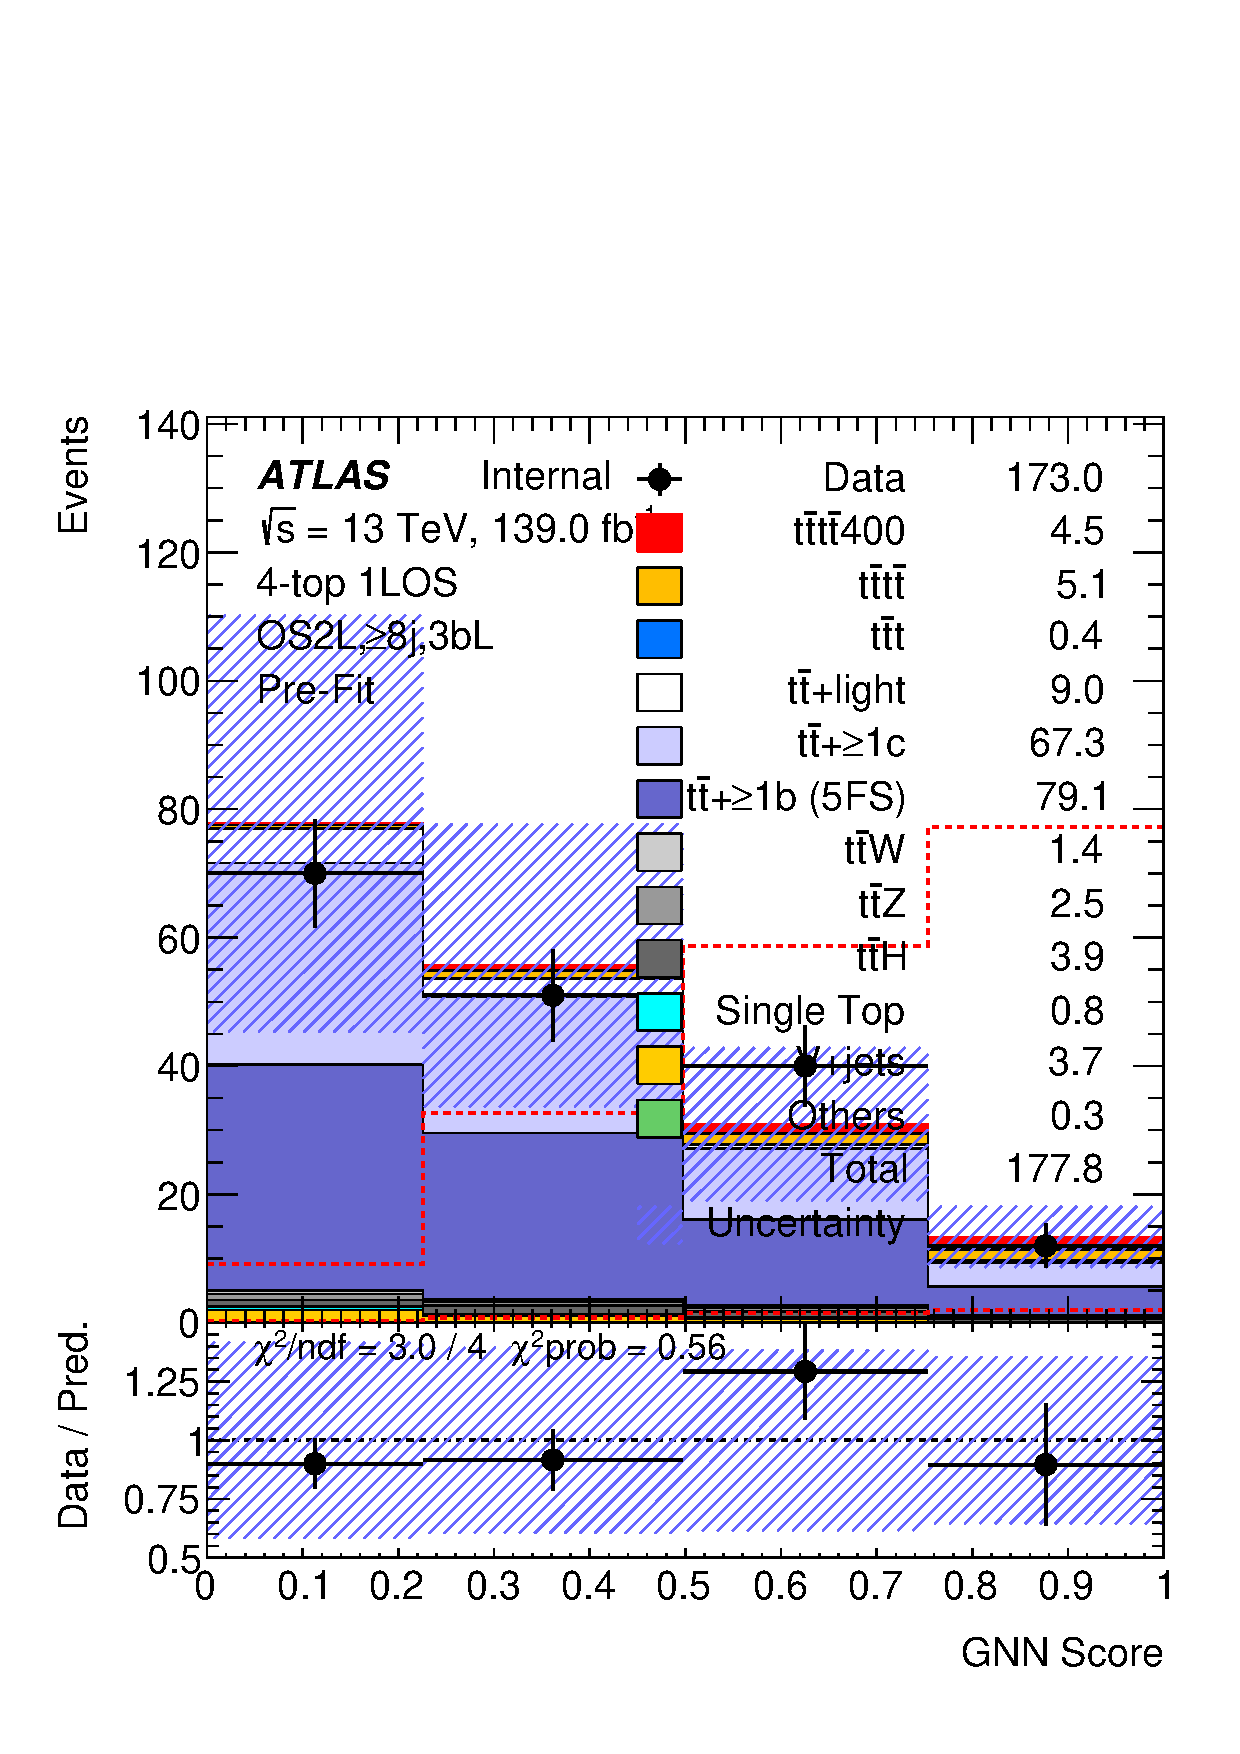
\includegraphics[width=0.31 \textwidth]{figures/fits/GNN/400/2L/data_unblindedSplusB/Plots/os2l_ge8j3bL.pdf} &
        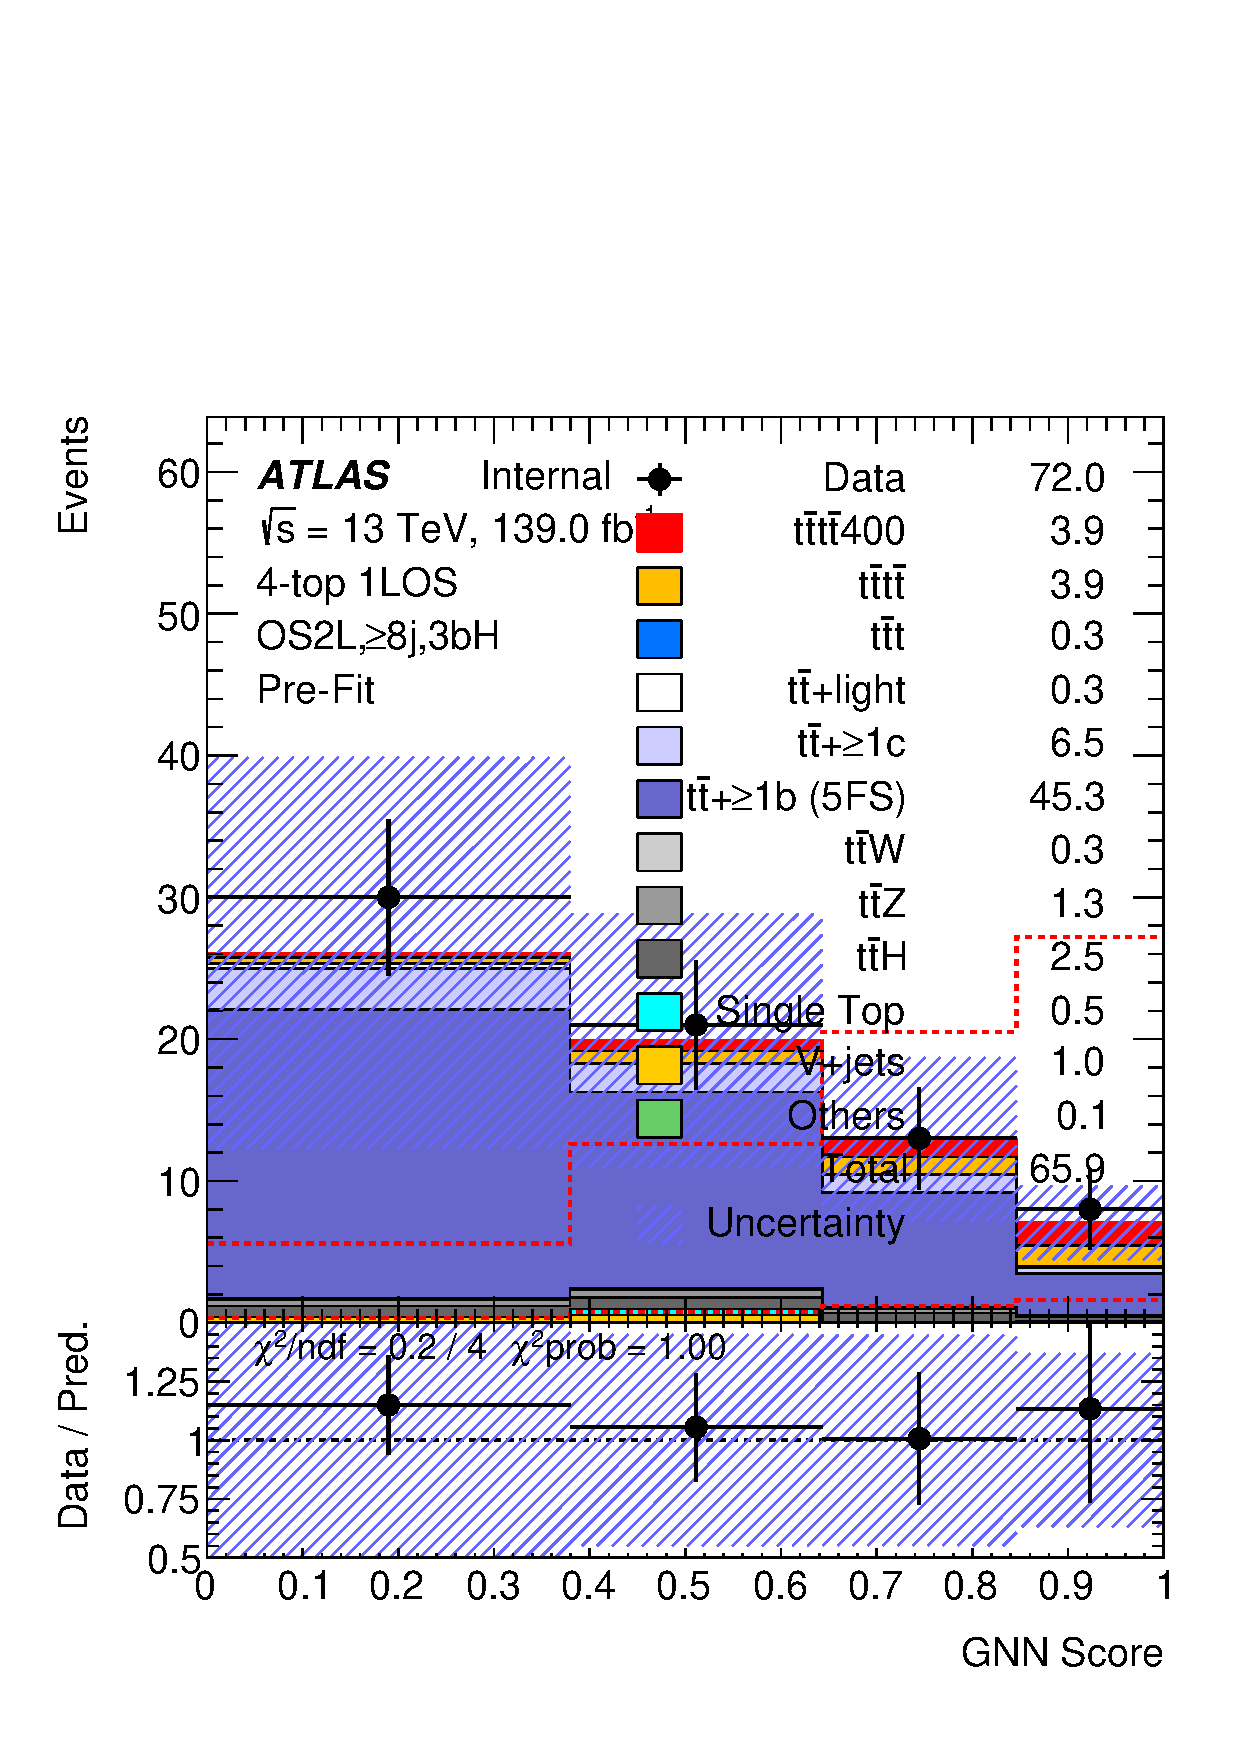
\includegraphics[width=0.31 \textwidth]{figures/fits/GNN/400/2L/data_unblindedSplusB/Plots/os2l_ge8j3bH.pdf} &
        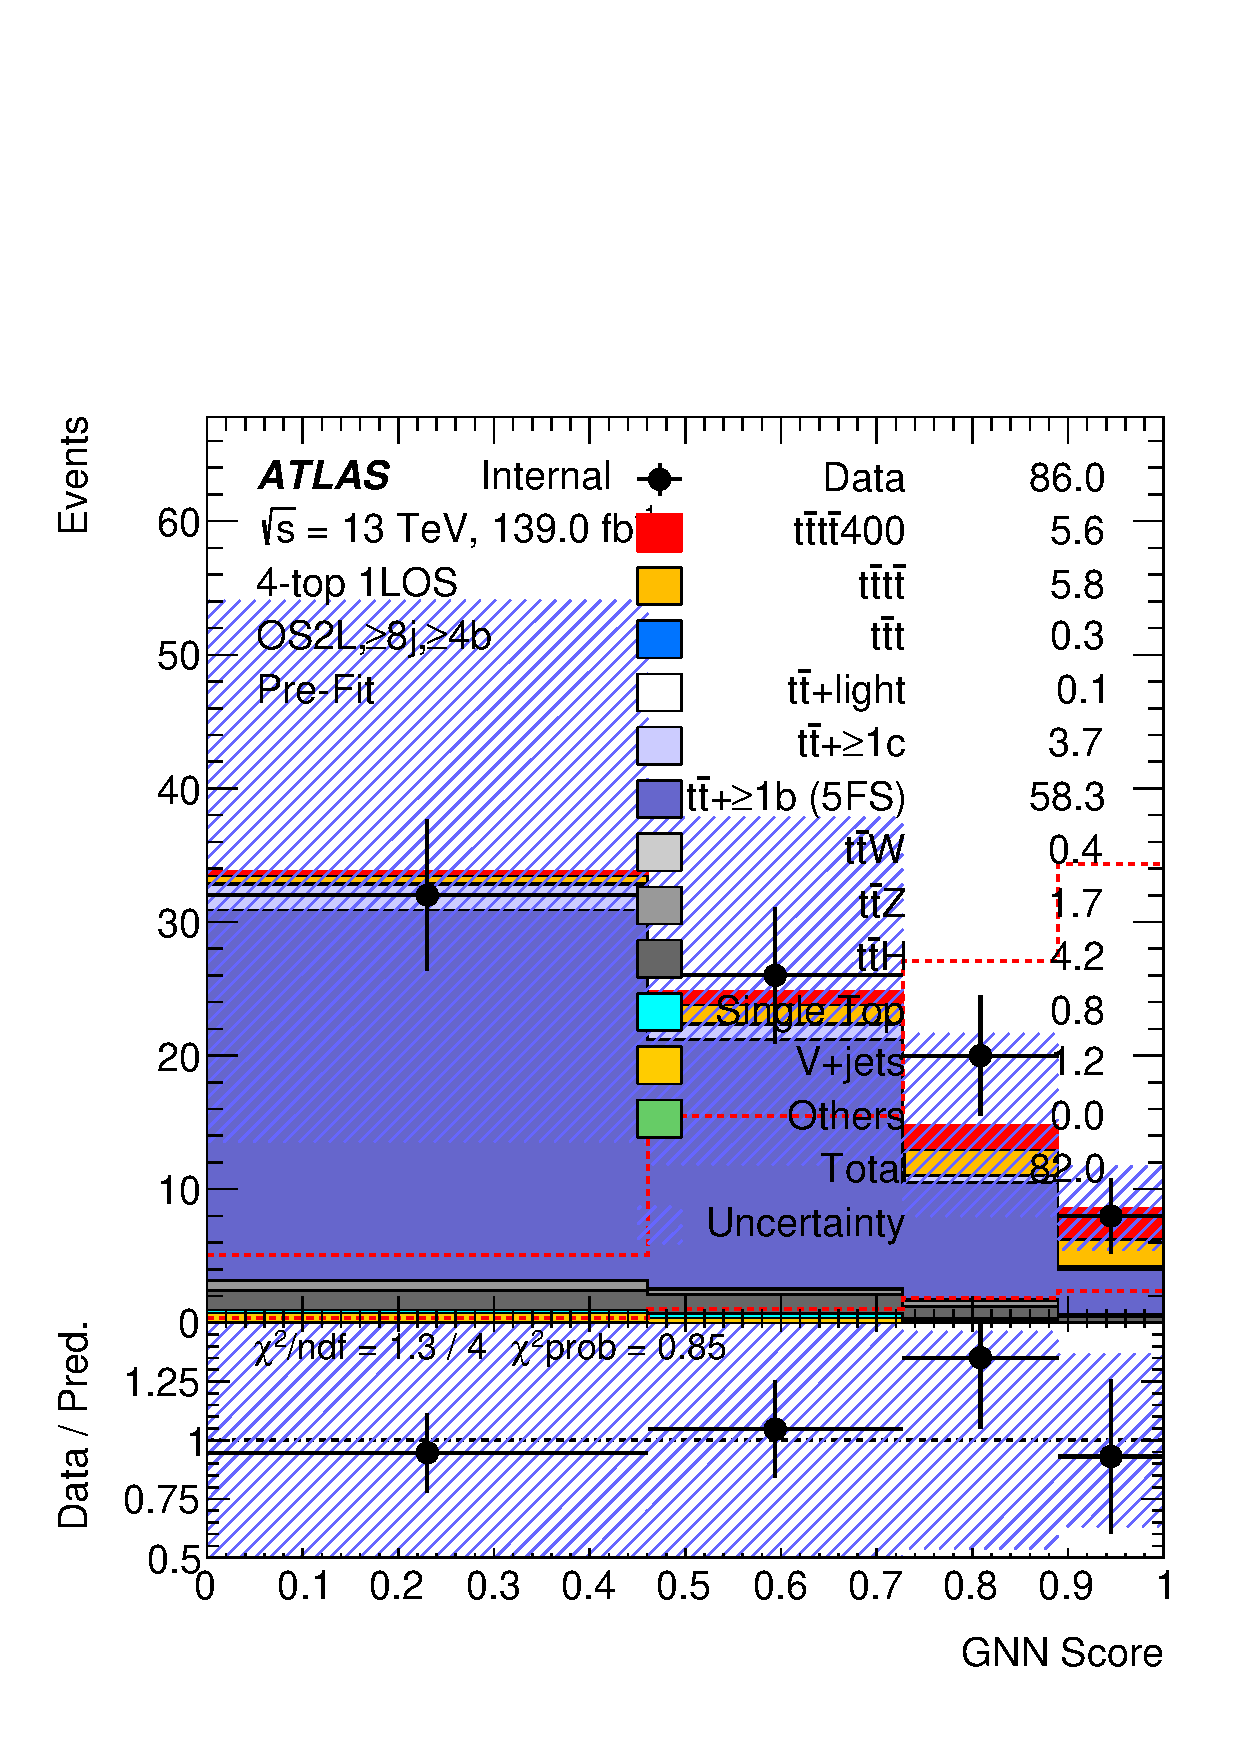
\includegraphics[width=0.31 \textwidth]{figures/fits/GNN/400/2L/data_unblindedSplusB/Plots/os2l_ge8jge4b.pdf} \\
        \end{tabular}
        \caption{\label{fig:Prefit_Yields_2L}Pre-fit distributions for 2LOS channel associated with different signal and background samples, compared with data yields. In general, MC samples and data have good agreement. The signal sample is normalised to a cross-section of 12 fb.}
\end{center}
\end{figure}


\begin{figure}[htbp!]
  \centering
  \begin{subfigure}[t]{0.32\textwidth}
    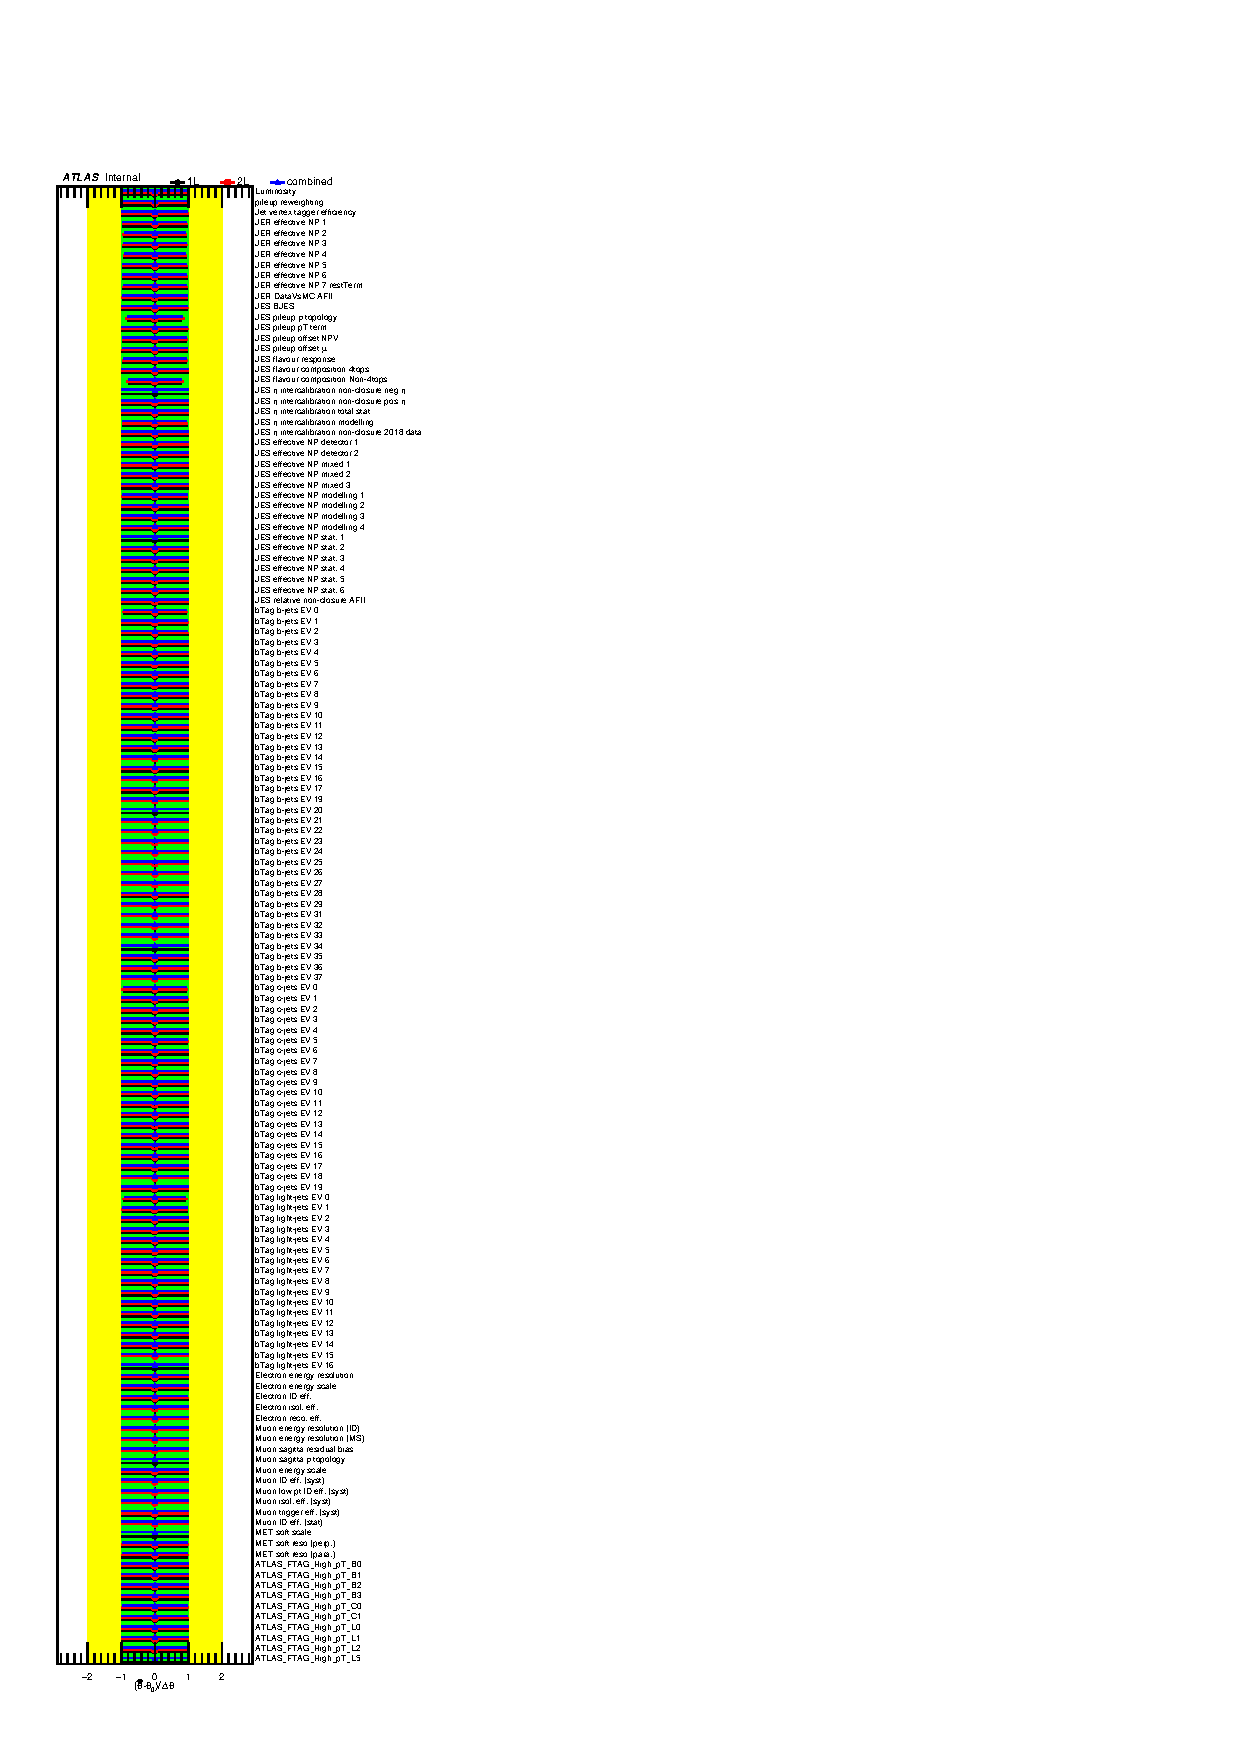
\includegraphics[width=\linewidth]{figures/fits/comparisons/selections/GNN/400/asimov/NuisPar_comp_Instrumental.pdf}
    \subcaption{mH=400\gev}
    \label{fig:Plain_NP_mH40}
  \end{subfigure}
  \begin{subfigure}[t]{0.32\textwidth}
    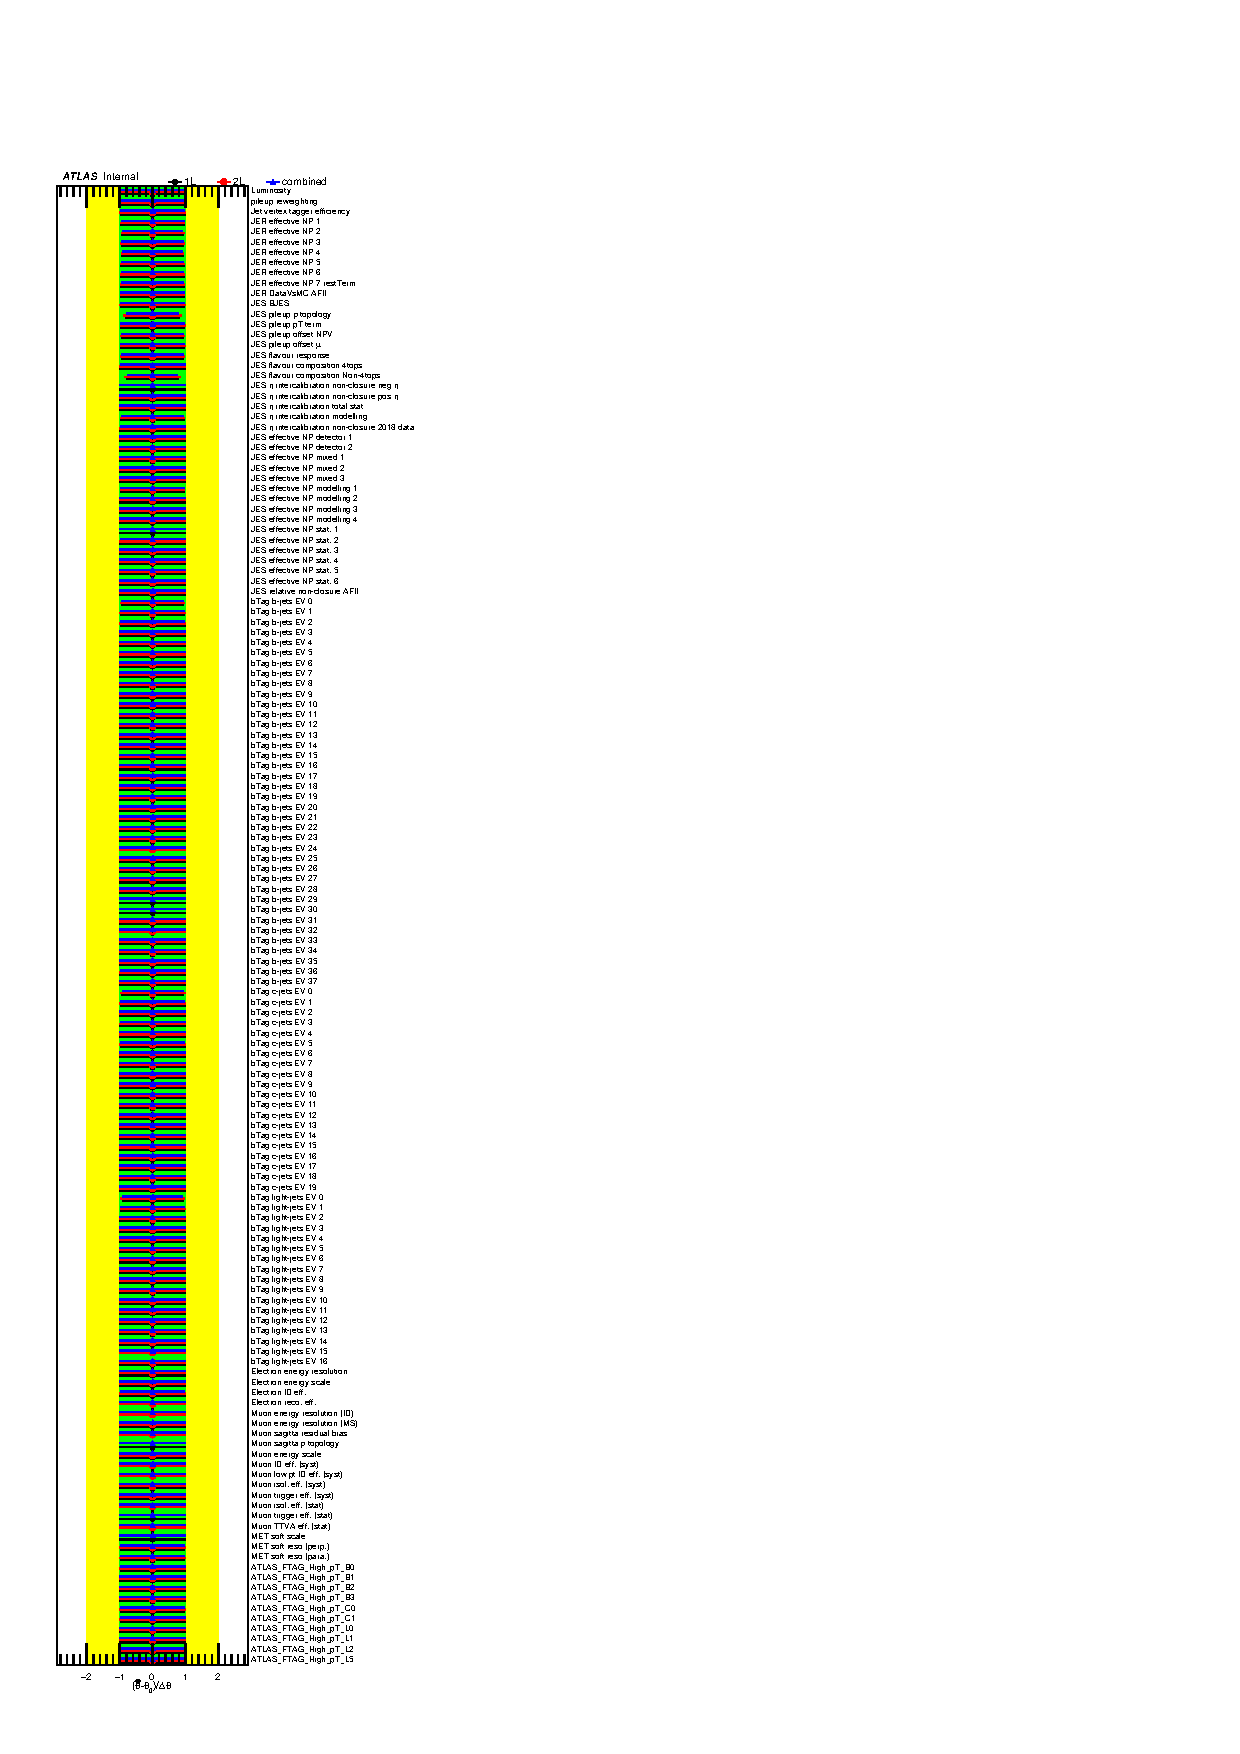
\includegraphics[width=\linewidth]{figures/fits/comparisons/selections/GNN/700/asimov/NuisPar_comp_Instrumental.pdf}
    \subcaption{mH=700\gev}
    \label{fig:Plain_NP_mH40}
  \end{subfigure}
  \begin{subfigure}[t]{0.32\textwidth}
    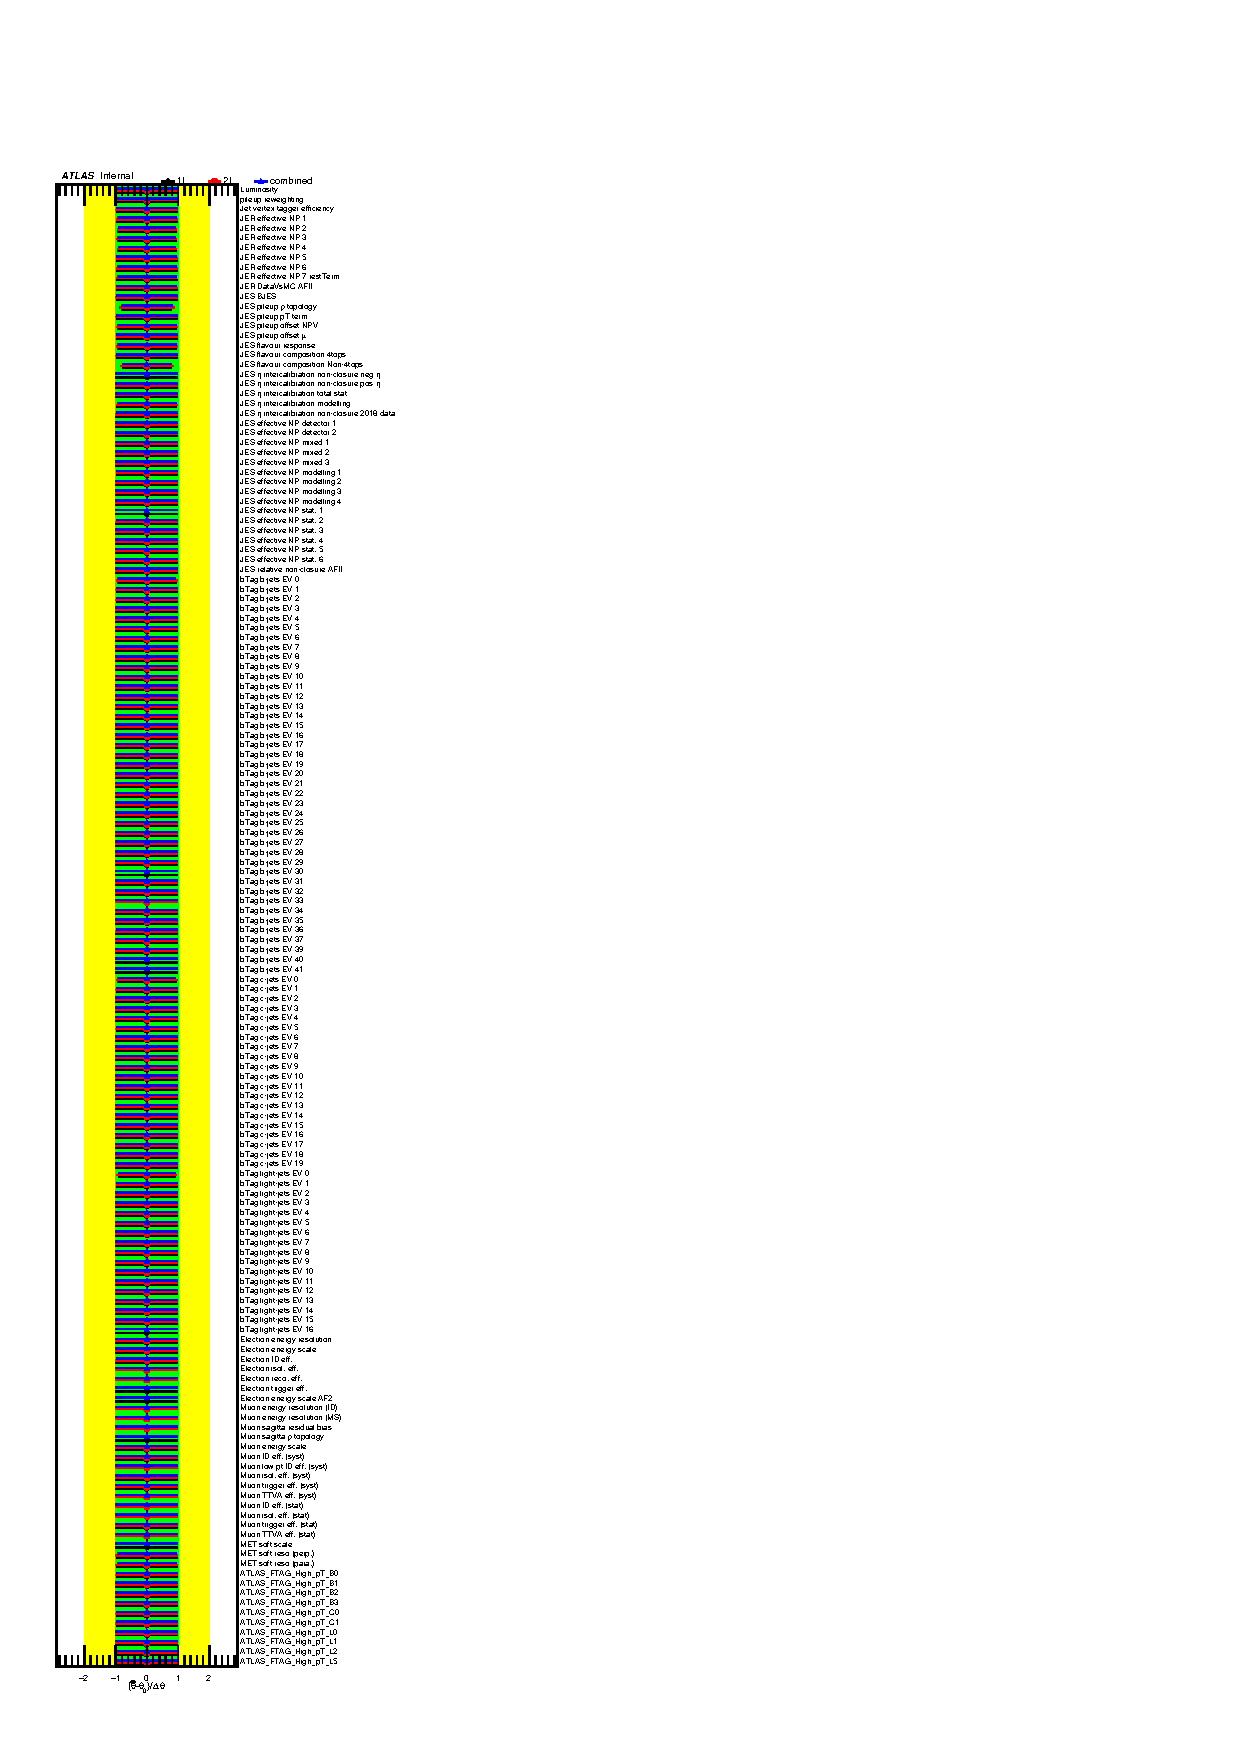
\includegraphics[width=\linewidth]{figures/fits/comparisons/selections/GNN/1000/asimov/NuisPar_comp_Instrumental.pdf}
    \subcaption{mH=1000\gev}
    \label{fig:Plain_NP_mH40}
  \end{subfigure}
  \caption{\label{fig:Plain_NP_instrumental}Fitted pulls and constraints for the nuisance parameters corresponding to the instrumental systematic uncertainties for the Plain Asimov fit for three mass points. Comparison is done for three fits: using only 1L regions, using only 2LOS regions and using all regions.}
\end{figure}


\begin{figure}[htbp!]
  \centering
  \begin{subfigure}[t]{0.32\textwidth}
    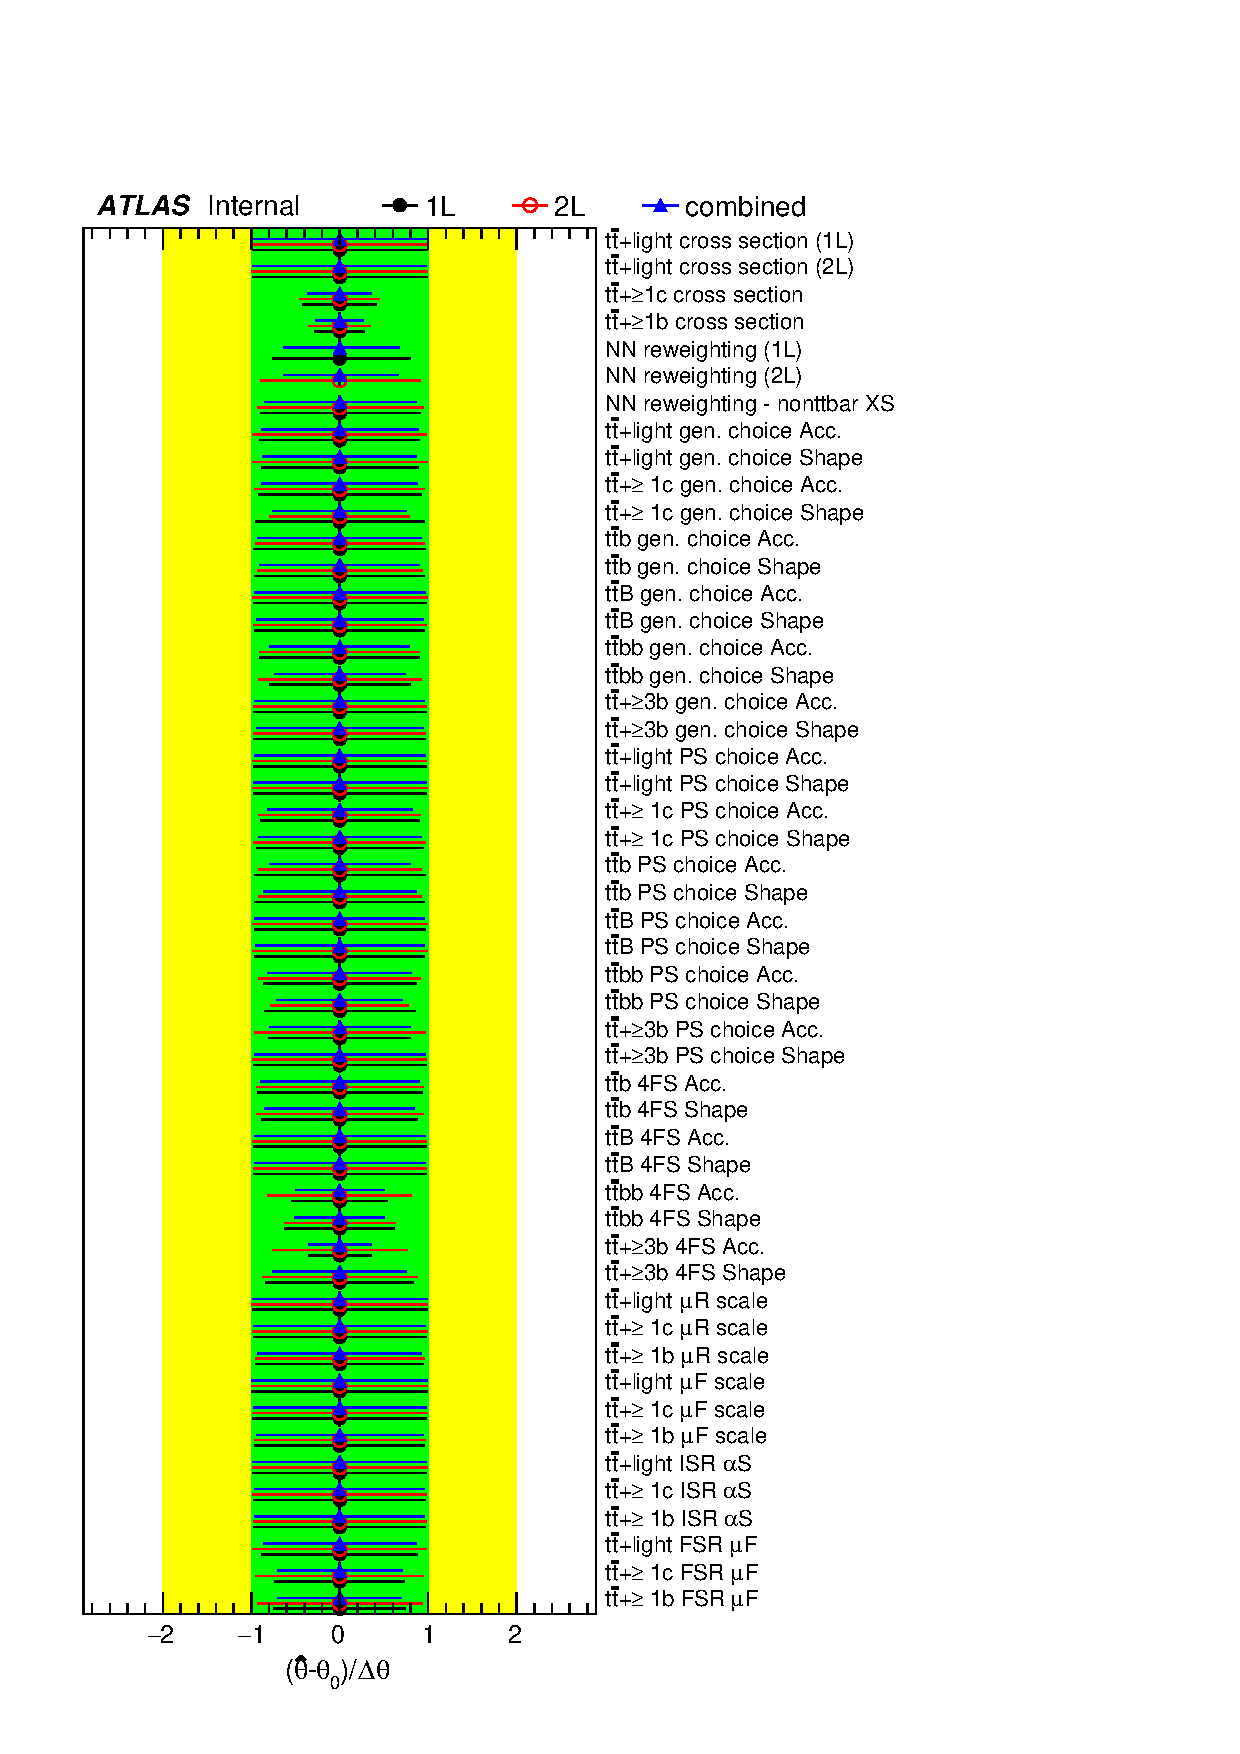
\includegraphics[width=\linewidth]{figures/fits/comparisons/selections/GNN/400/asimov/NuisPar_comp_ttbar.pdf}
    \subcaption{mH=400\gev}
    \label{fig:Plain_NP_mH40}
  \end{subfigure}
  \begin{subfigure}[t]{0.32\textwidth}
    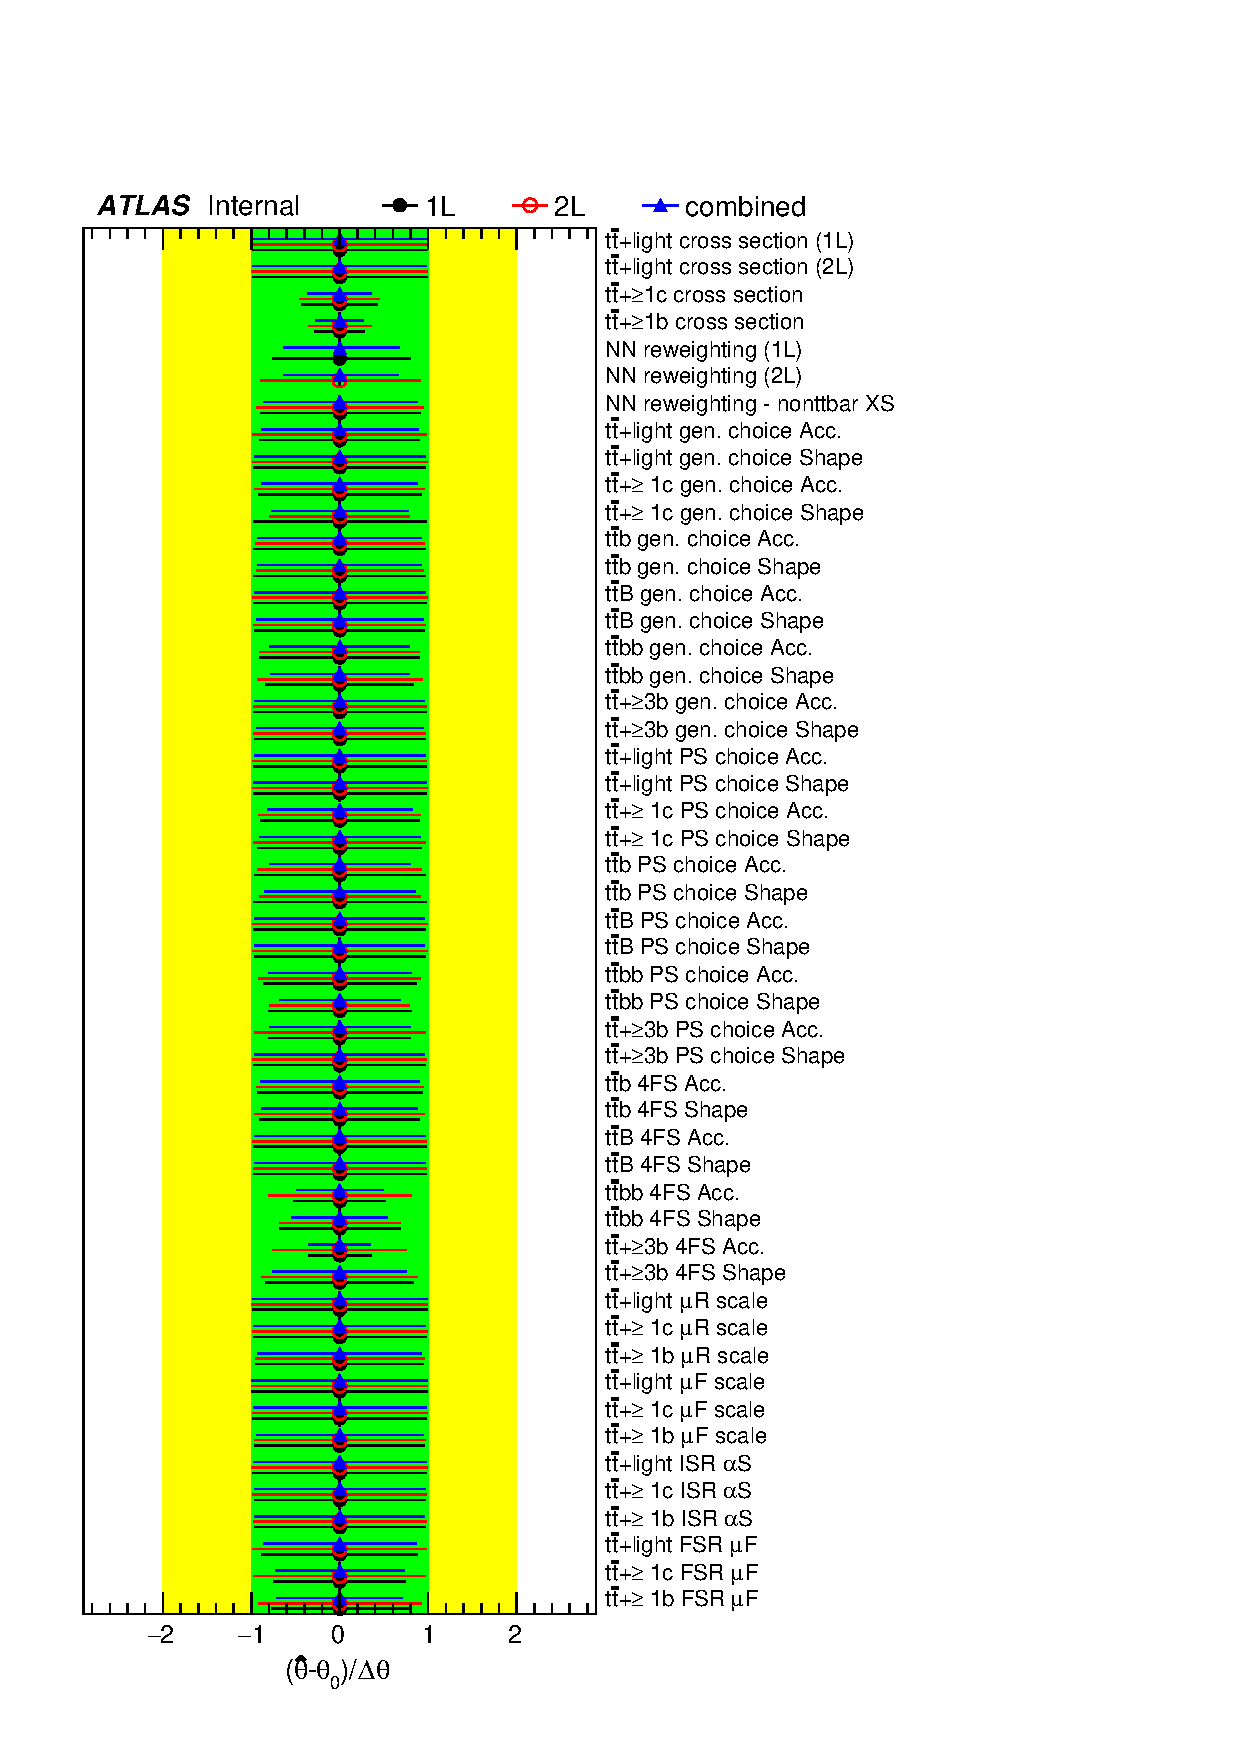
\includegraphics[width=\linewidth]{figures/fits/comparisons/selections/GNN/700/asimov/NuisPar_comp_ttbar.pdf}
    \subcaption{mH=700\gev}
    \label{fig:Plain_NP_mH40}
  \end{subfigure}
  \begin{subfigure}[t]{0.32\textwidth}
    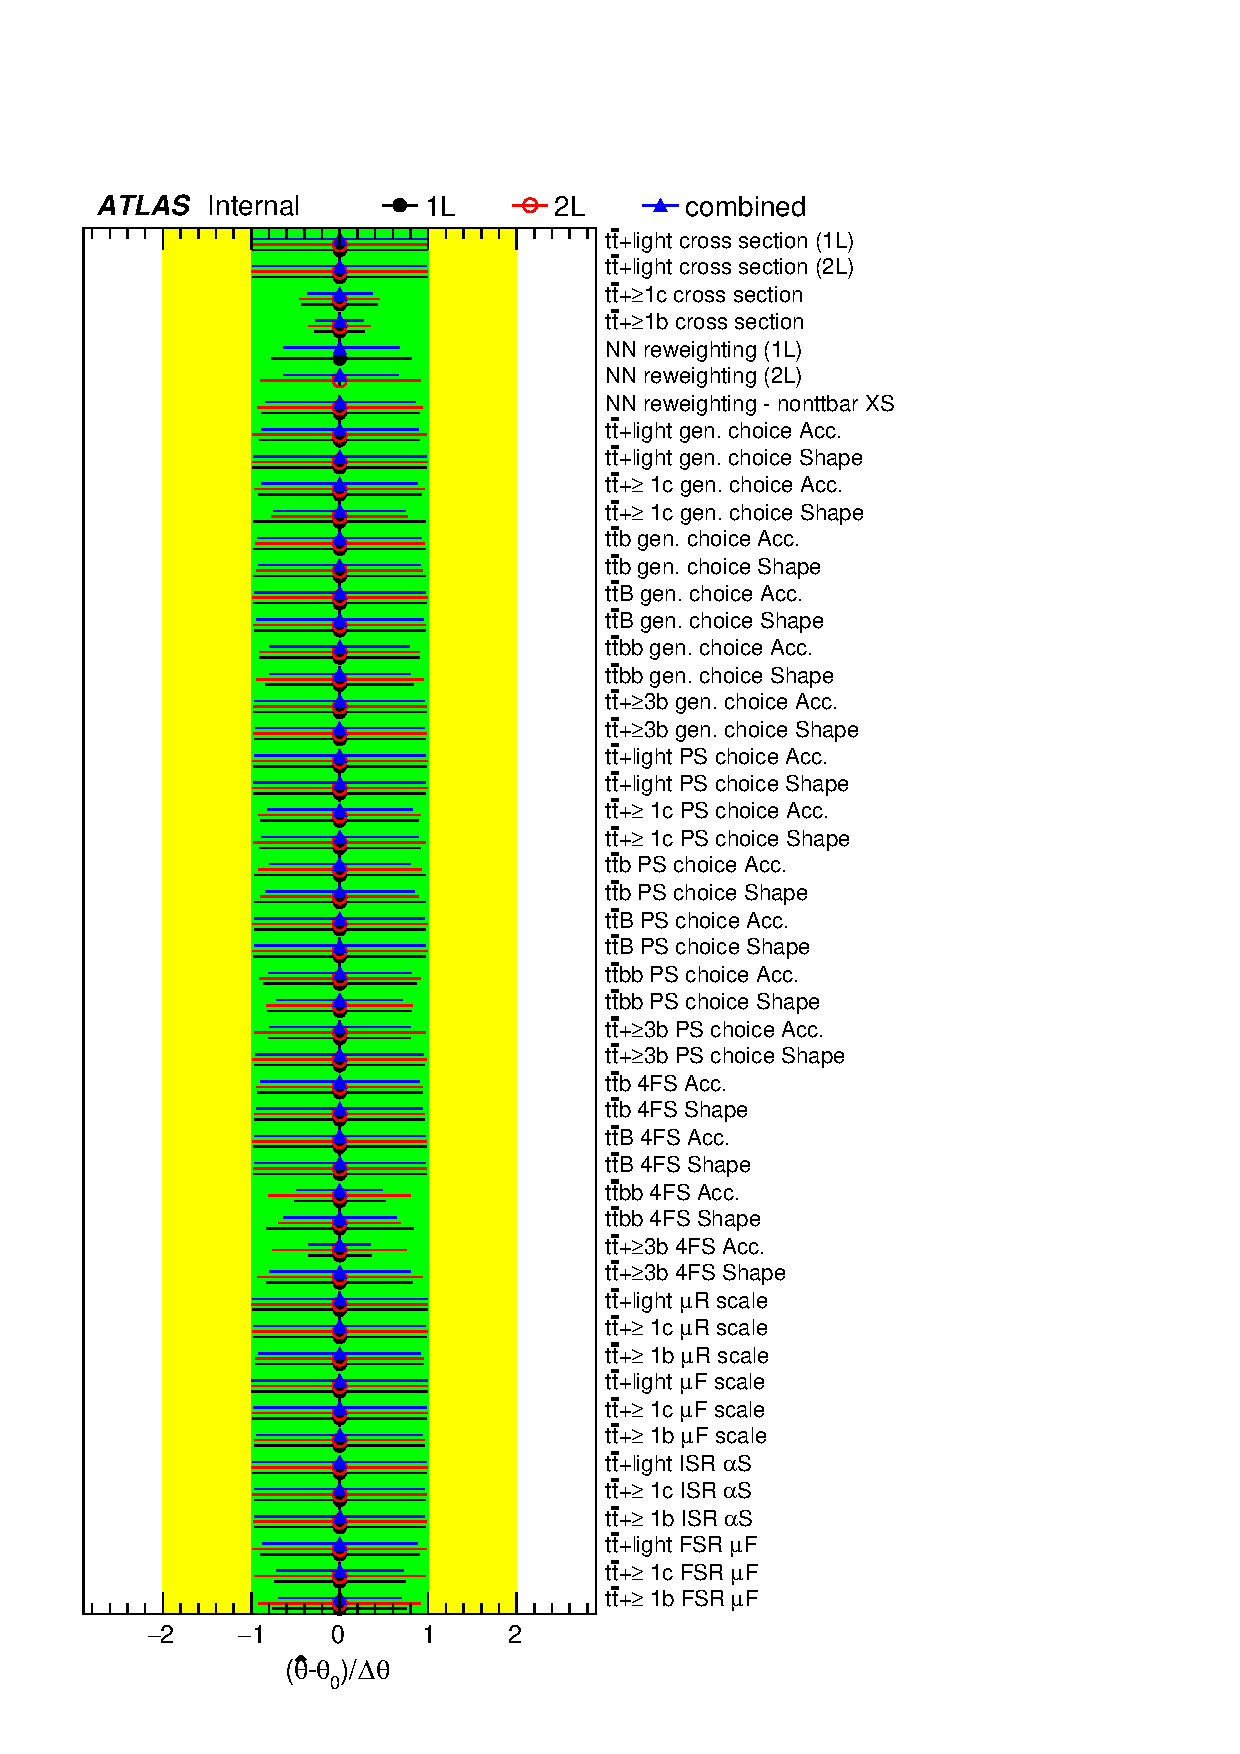
\includegraphics[width=\linewidth]{figures/fits/comparisons/selections/GNN/1000/asimov/NuisPar_comp_ttbar.pdf}
    \subcaption{mH=1000\gev}
    \label{fig:Plain_NP_mH40}
  \end{subfigure}
  \caption{\label{fig:Plain_NP_ttbar}Fitted pulls and constraints for the nuisance parameters corresponding to the \ttbar systematic uncertainties for the Plain Asimov fit for three mass points. Comparison is done for three fits: using only 1L regions, using only 2LOS regions and using all regions.}
\end{figure}


\begin{figure}[htbp!]
  \centering
  \begin{subfigure}[t]{0.32\textwidth}
    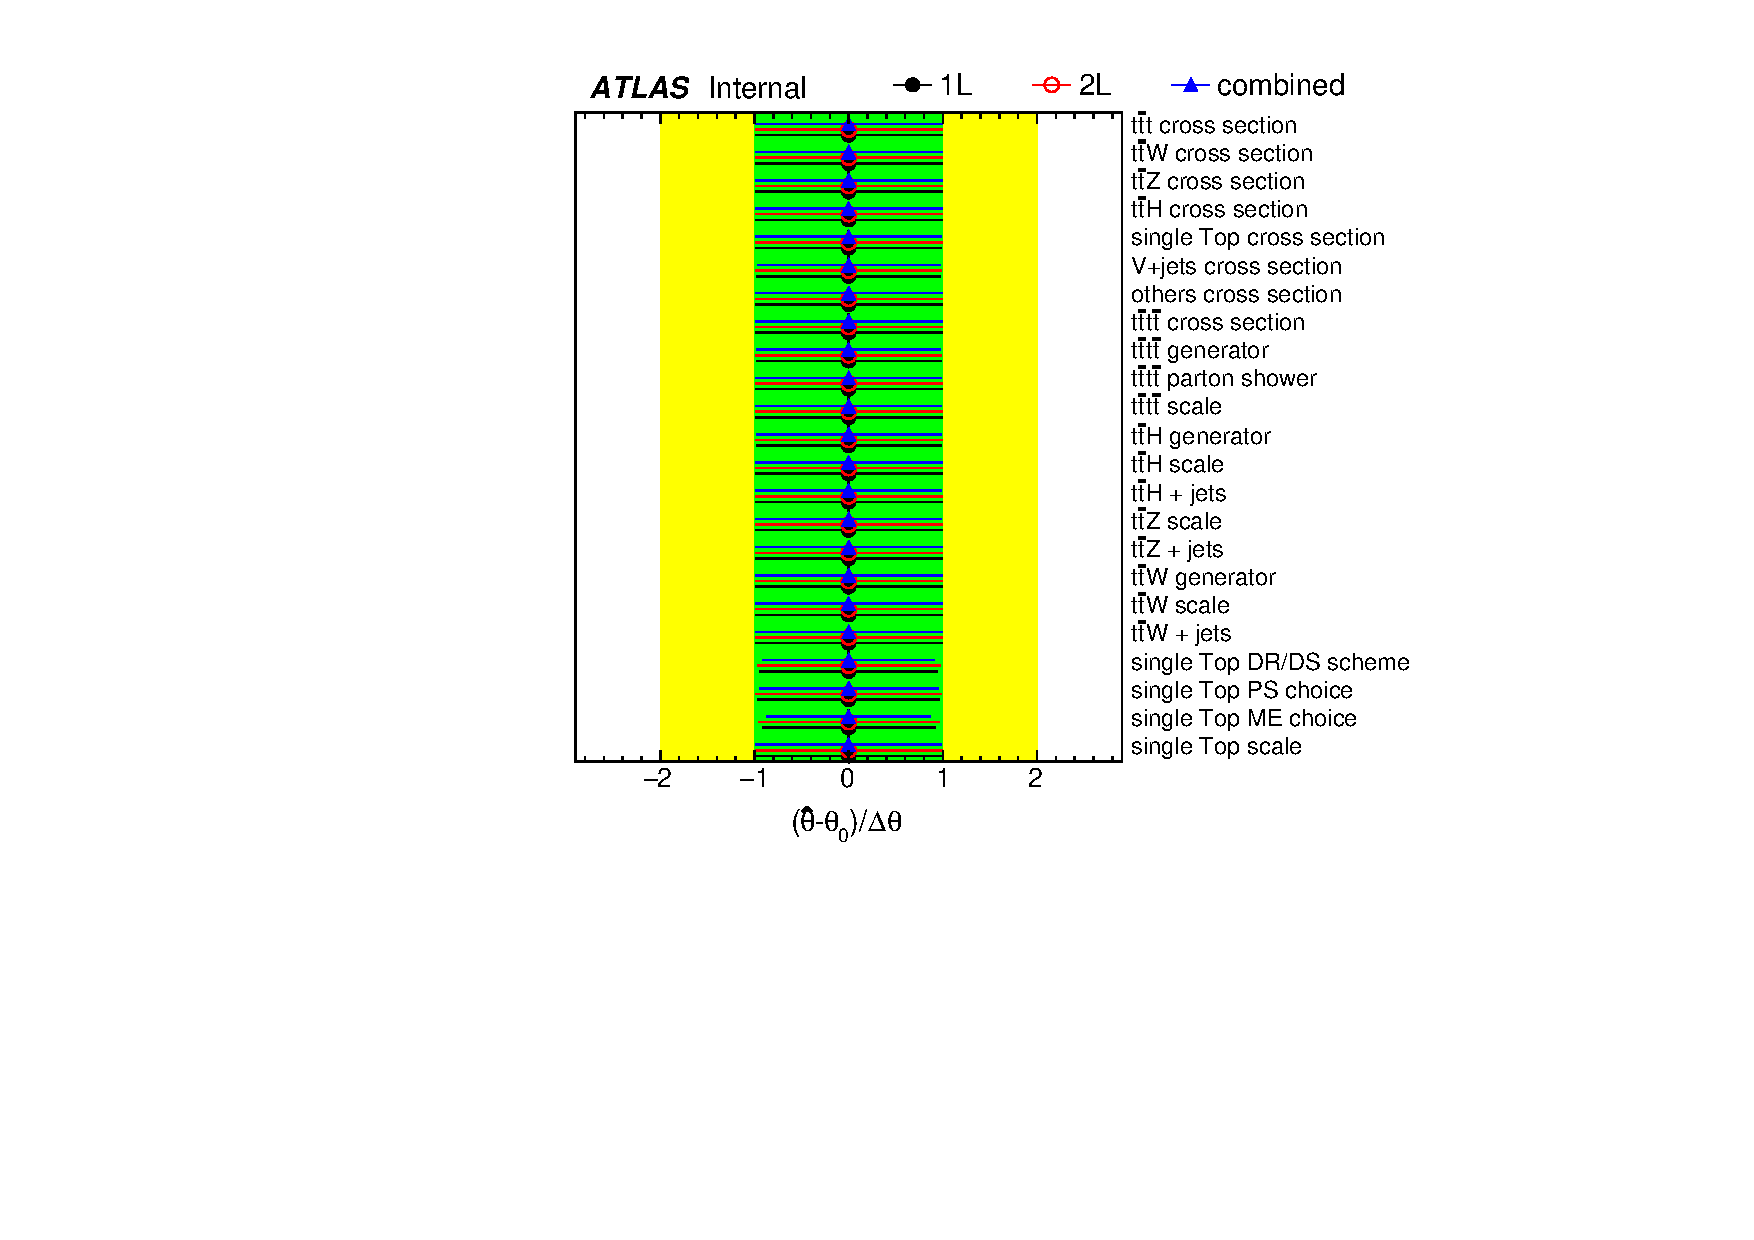
\includegraphics[width=\linewidth]{figures/fits/comparisons/selections/GNN/400/asimov/NuisPar_comp_Other.pdf}
    \subcaption{mH=400\gev}
    \label{fig:Plain_NP_mH40}
  \end{subfigure}
  \begin{subfigure}[t]{0.32\textwidth}
    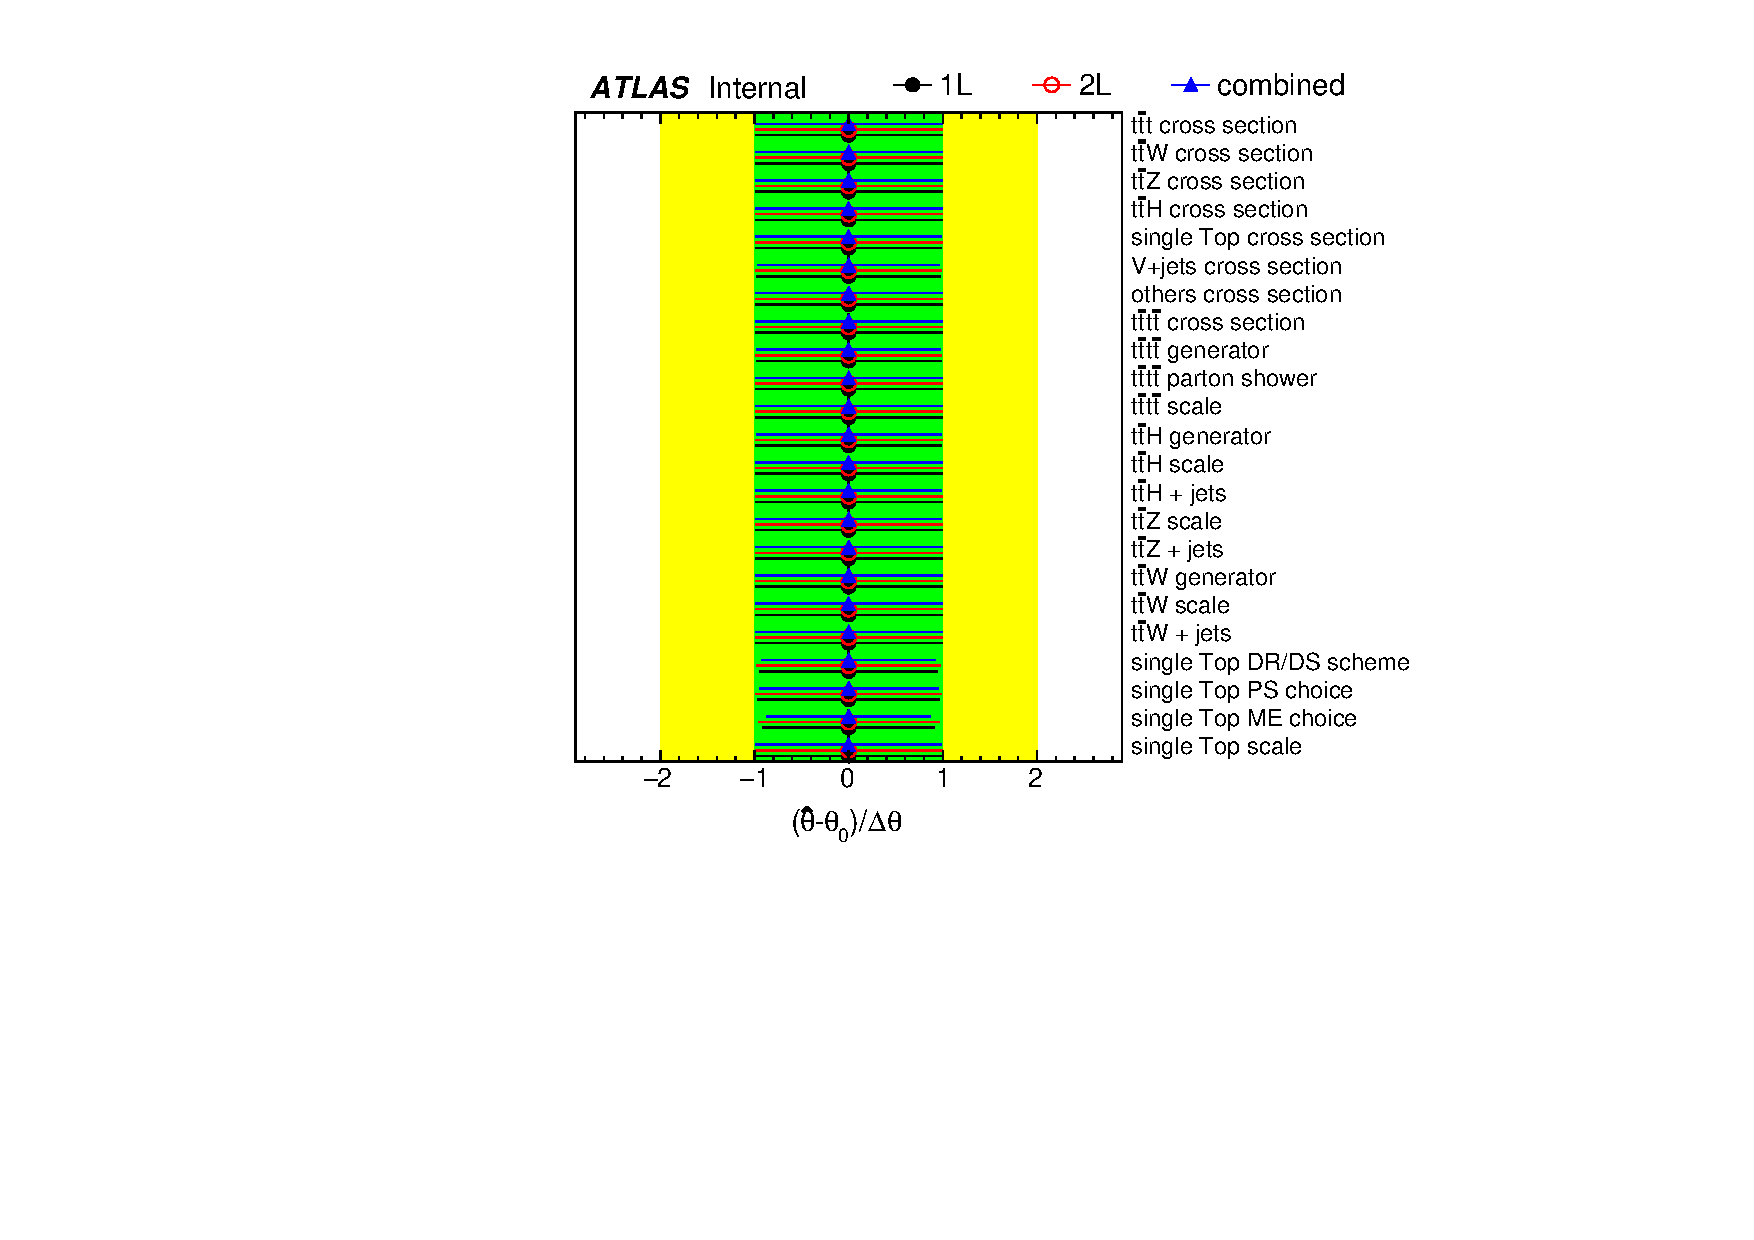
\includegraphics[width=\linewidth]{figures/fits/comparisons/selections/GNN/700/asimov/NuisPar_comp_Other.pdf}
    \subcaption{mH=700\gev}
    \label{fig:Plain_NP_mH40}
  \end{subfigure}
  \begin{subfigure}[t]{0.32\textwidth}
    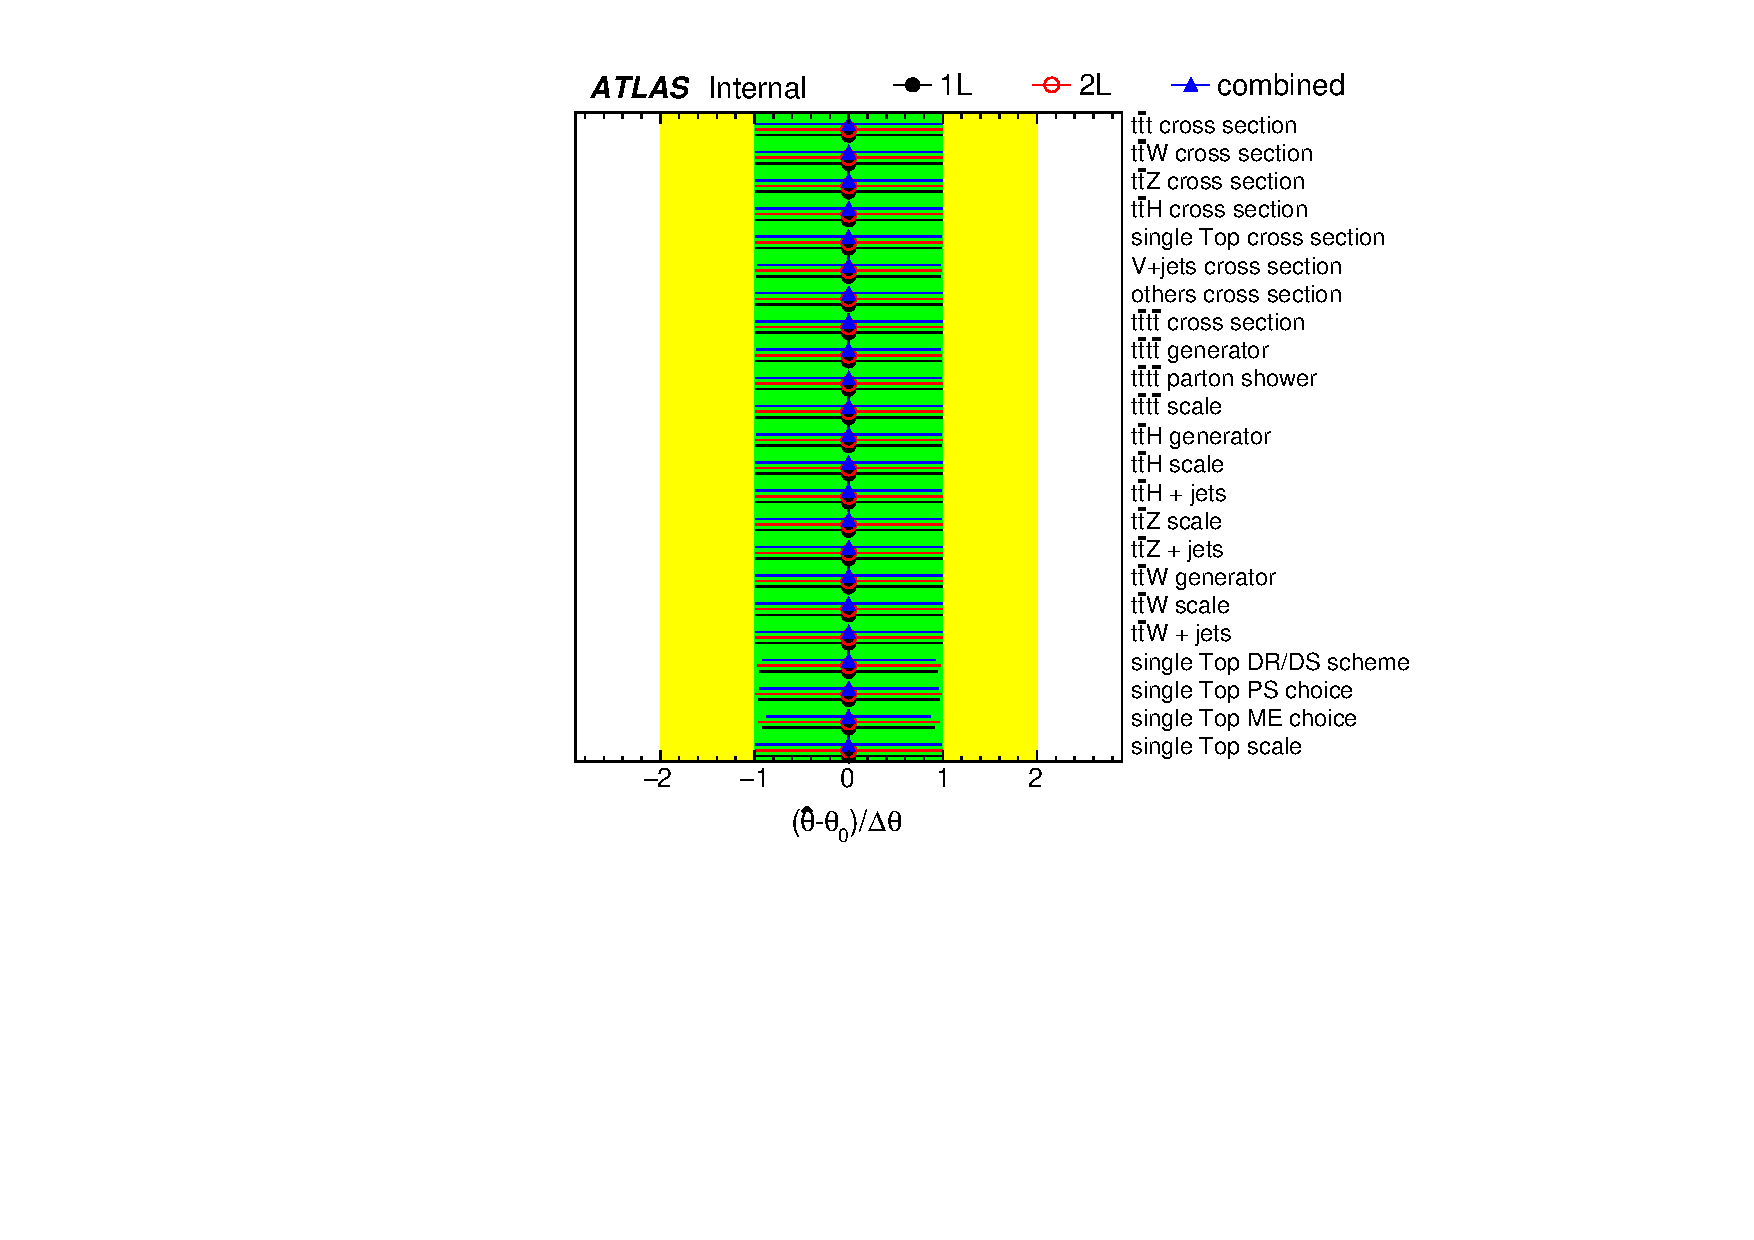
\includegraphics[width=\linewidth]{figures/fits/comparisons/selections/GNN/1000/asimov/NuisPar_comp_Other.pdf}
    \subcaption{mH=1000\gev}
    \label{fig:Plain_NP_mH40}
  \end{subfigure}
  \caption{\label{fig:Plain_NP_other}Fitted pulls and constraints for the nuisance parameters corresponding to the non-\ttbar background systematic uncertainties for the Plain Asimov fit for three mass points. Comparison is done for three fits: using only 1L regions, using only 2LOS regions and using all regions.}
\end{figure}

\begin{figure}[htbp!]
  \centering
  \begin{subfigure}[t]{0.32\textwidth}
    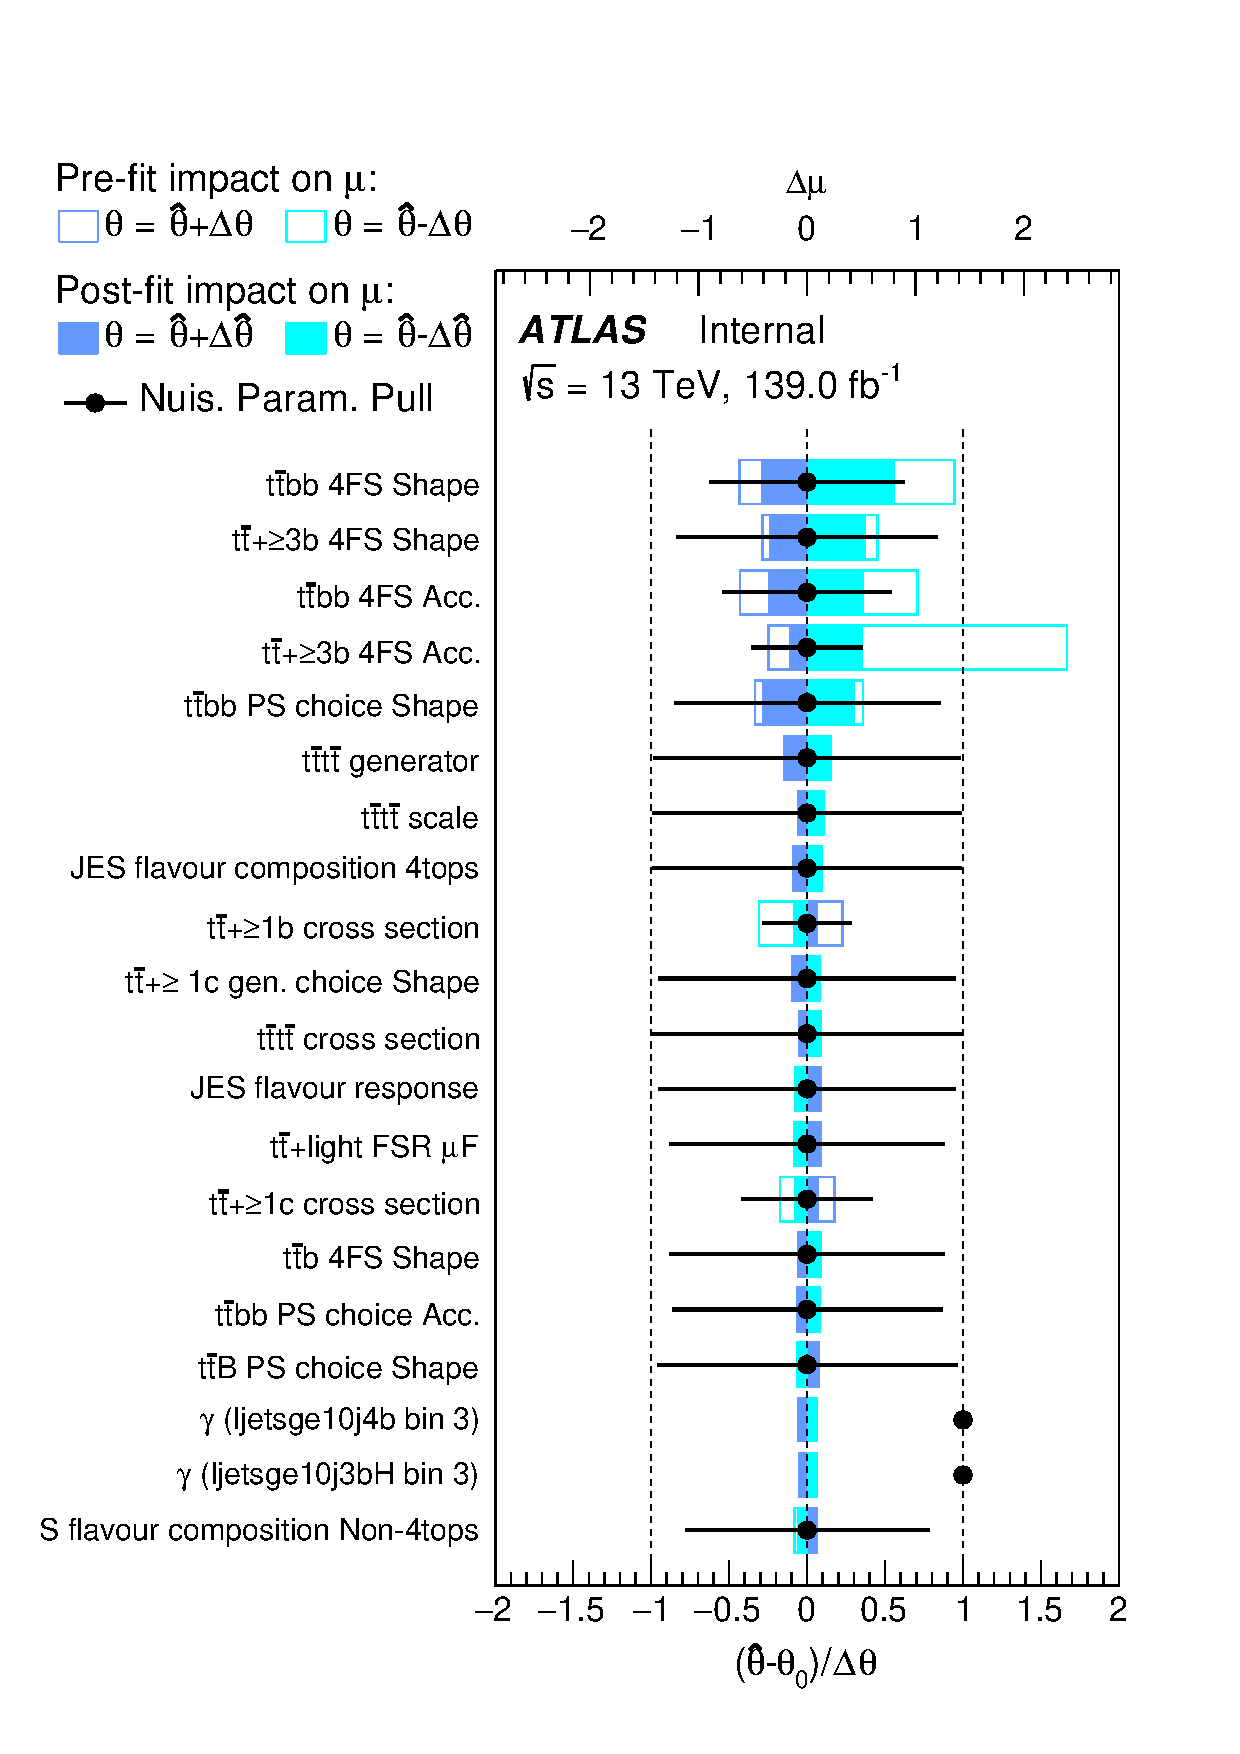
\includegraphics[width=\linewidth]{figures/fits/GNN/400/1L/asimov/Ranking_mu_tttt.pdf}
     \caption{\label{fig:Ranking_mH400_Asimov_1L}1L }
  \end{subfigure}
  \begin{subfigure}[t]{0.32\textwidth}
    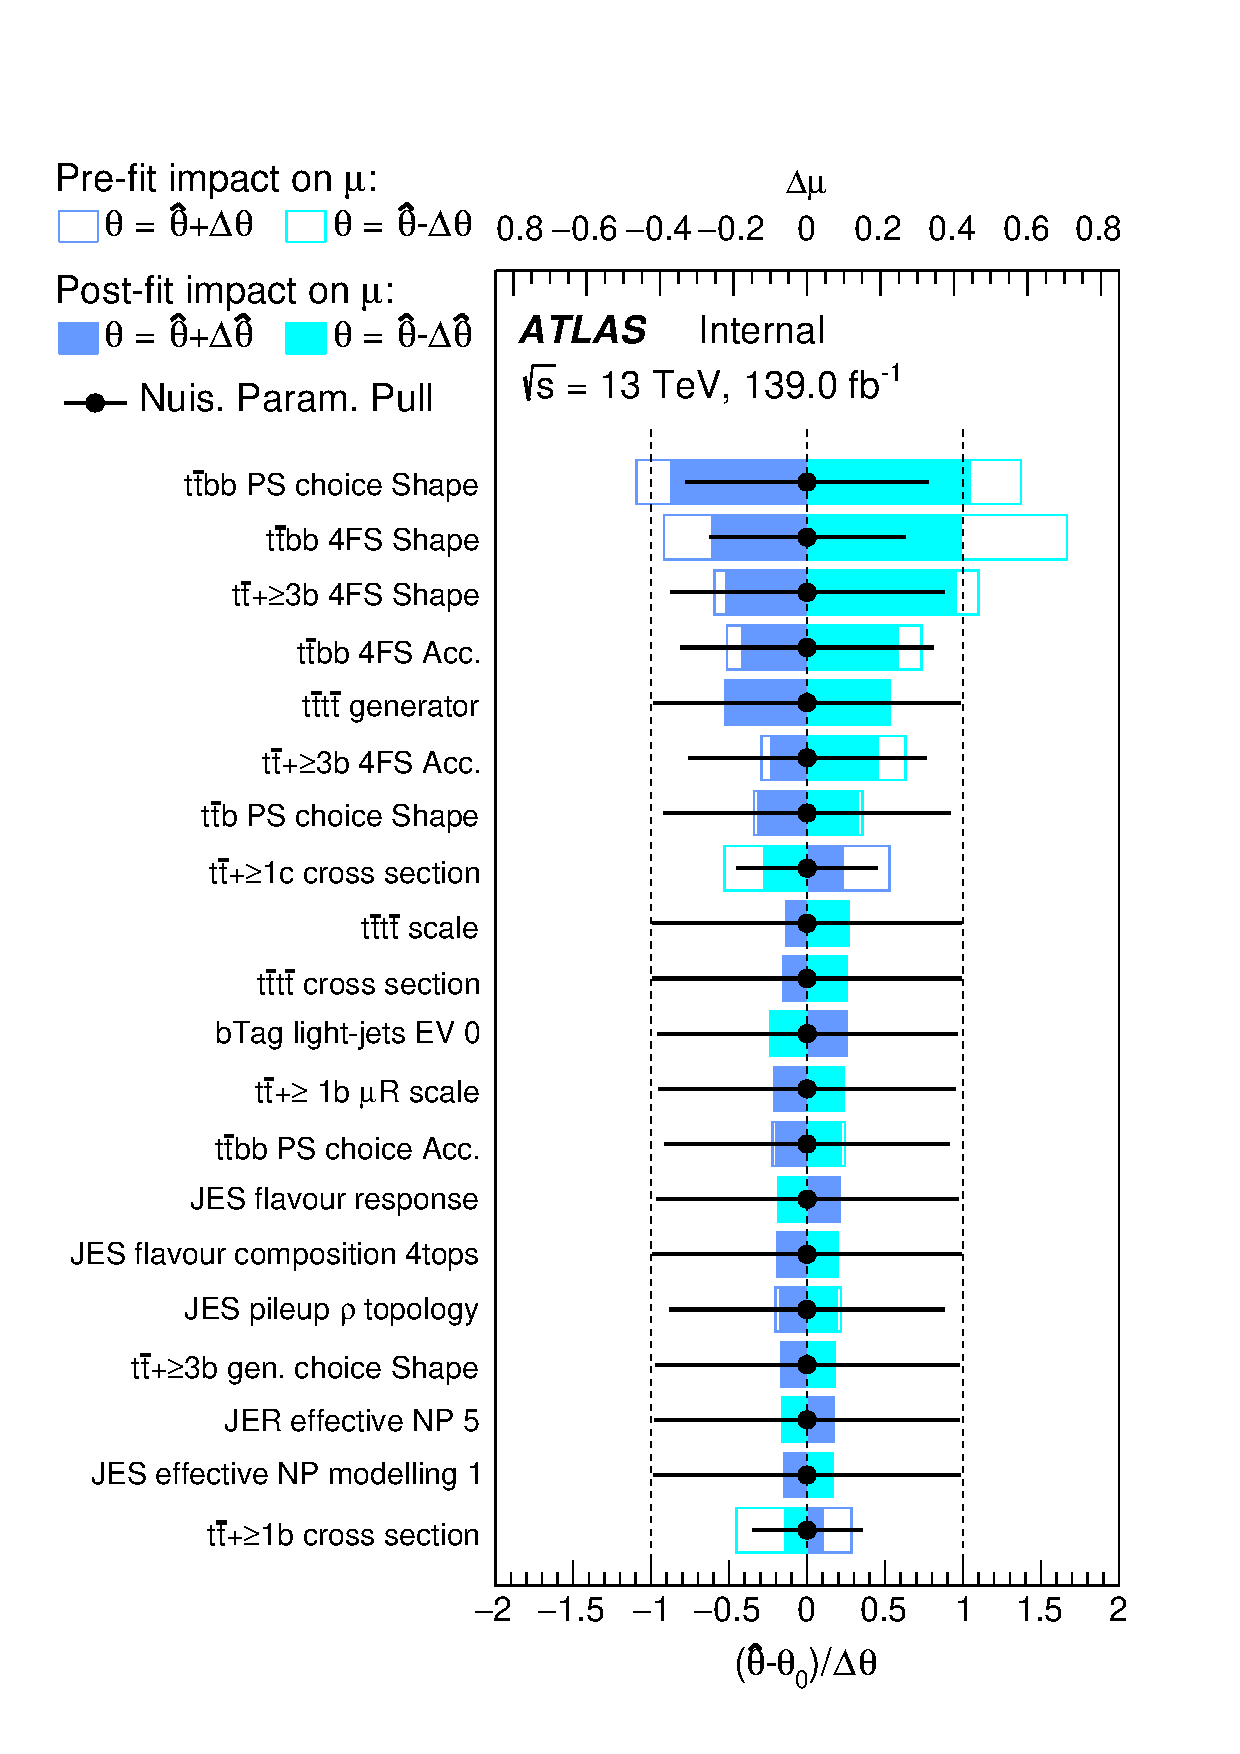
\includegraphics[width=\linewidth]{figures/fits/GNN/400/2L/asimov/Ranking_mu_tttt.pdf}
     \caption{\label{fig:Ranking_mH400_Asimov_2L}2L }
  \end{subfigure}
  \begin{subfigure}[t]{0.32\textwidth}
    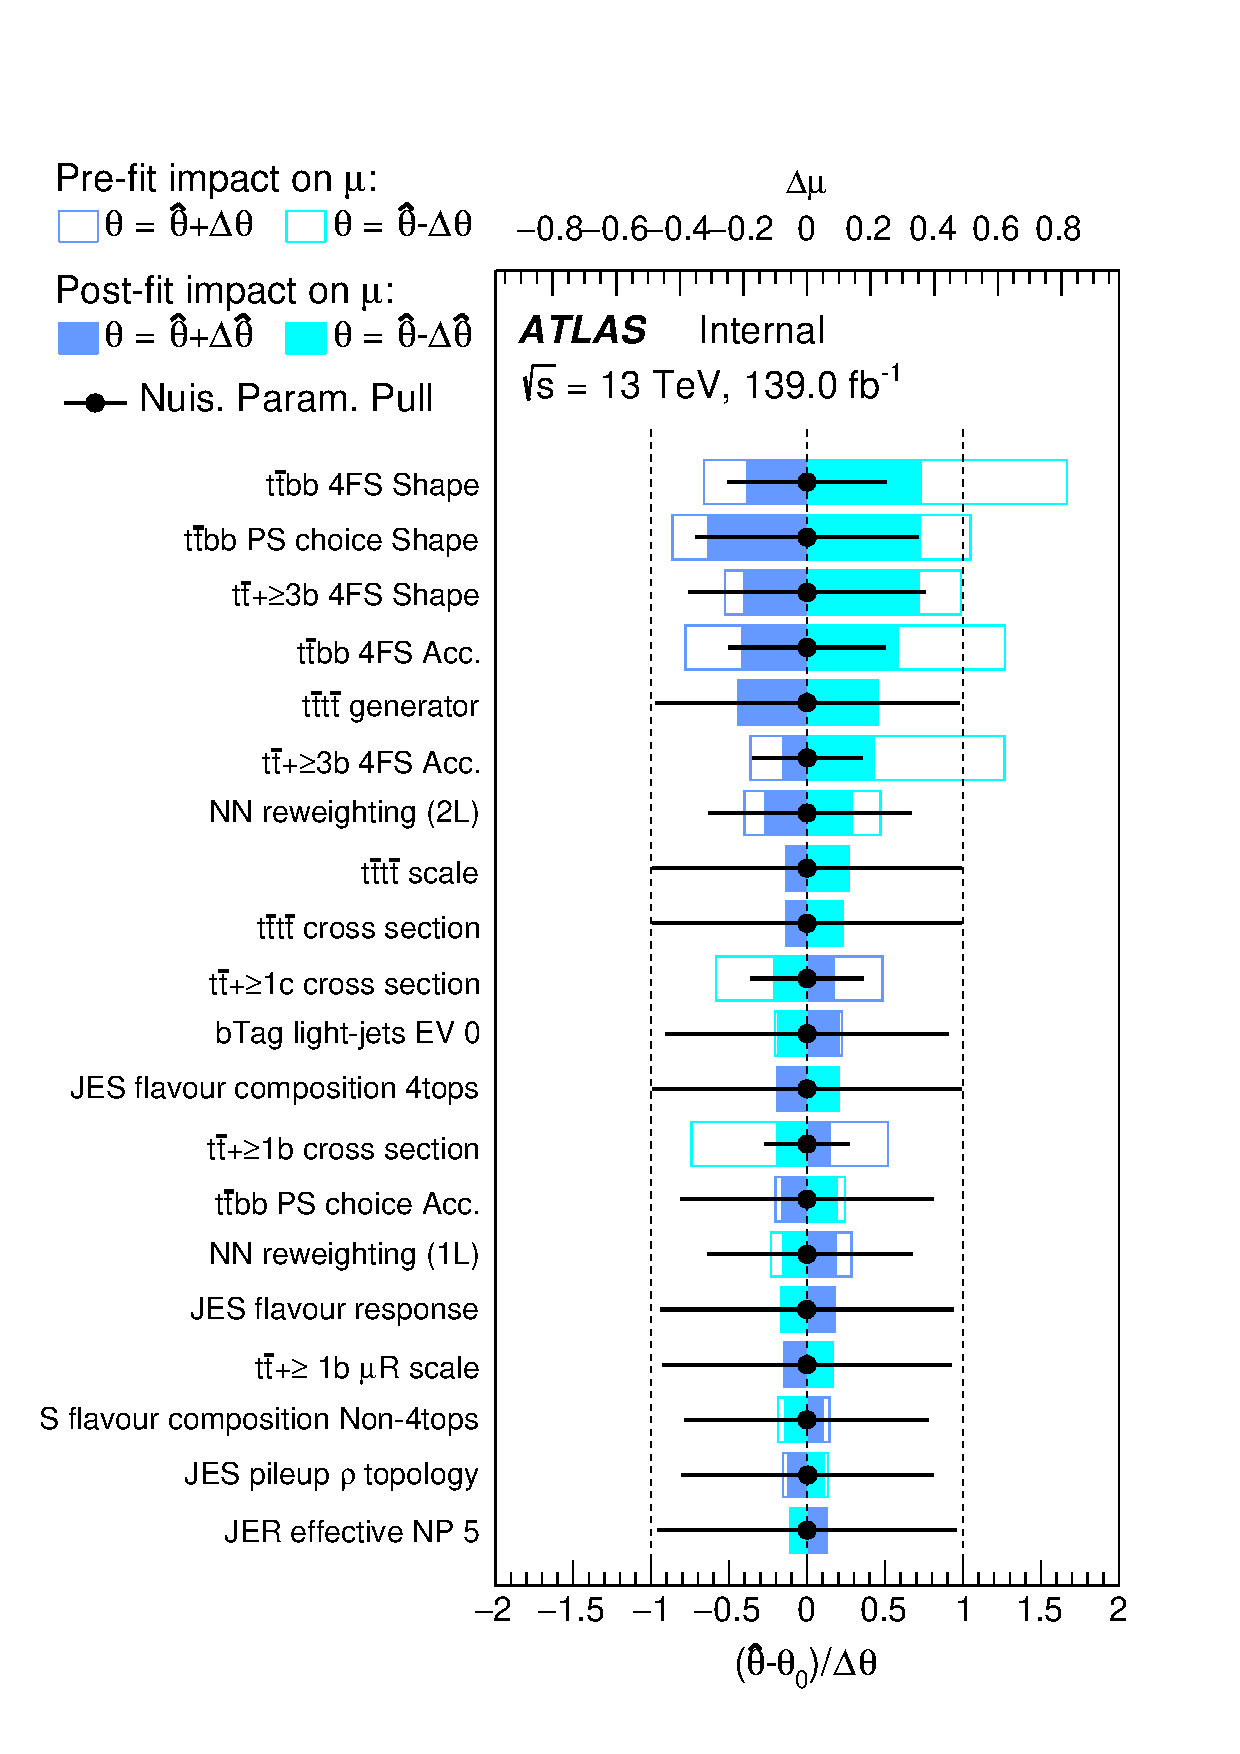
\includegraphics[width=\linewidth]{figures/fits/GNN/400/all/asimov/Ranking_mu_tttt.pdf}
     \caption{\label{fig:Ranking_mH400_Asimov_all}1L+2L }
  \end{subfigure}
  \caption{\label{fig:Ranking_mH400_Asimov}Fitted pulls and constraints for the nuisance parameters ranked by their impact for mH=400\gev for three types of Asimov fit: using only 1L regions, using only 2L regions and using all regions.}
\end{figure}


\begin{figure}[htbp!]
  \centering
  \begin{subfigure}[t]{0.32\textwidth}
    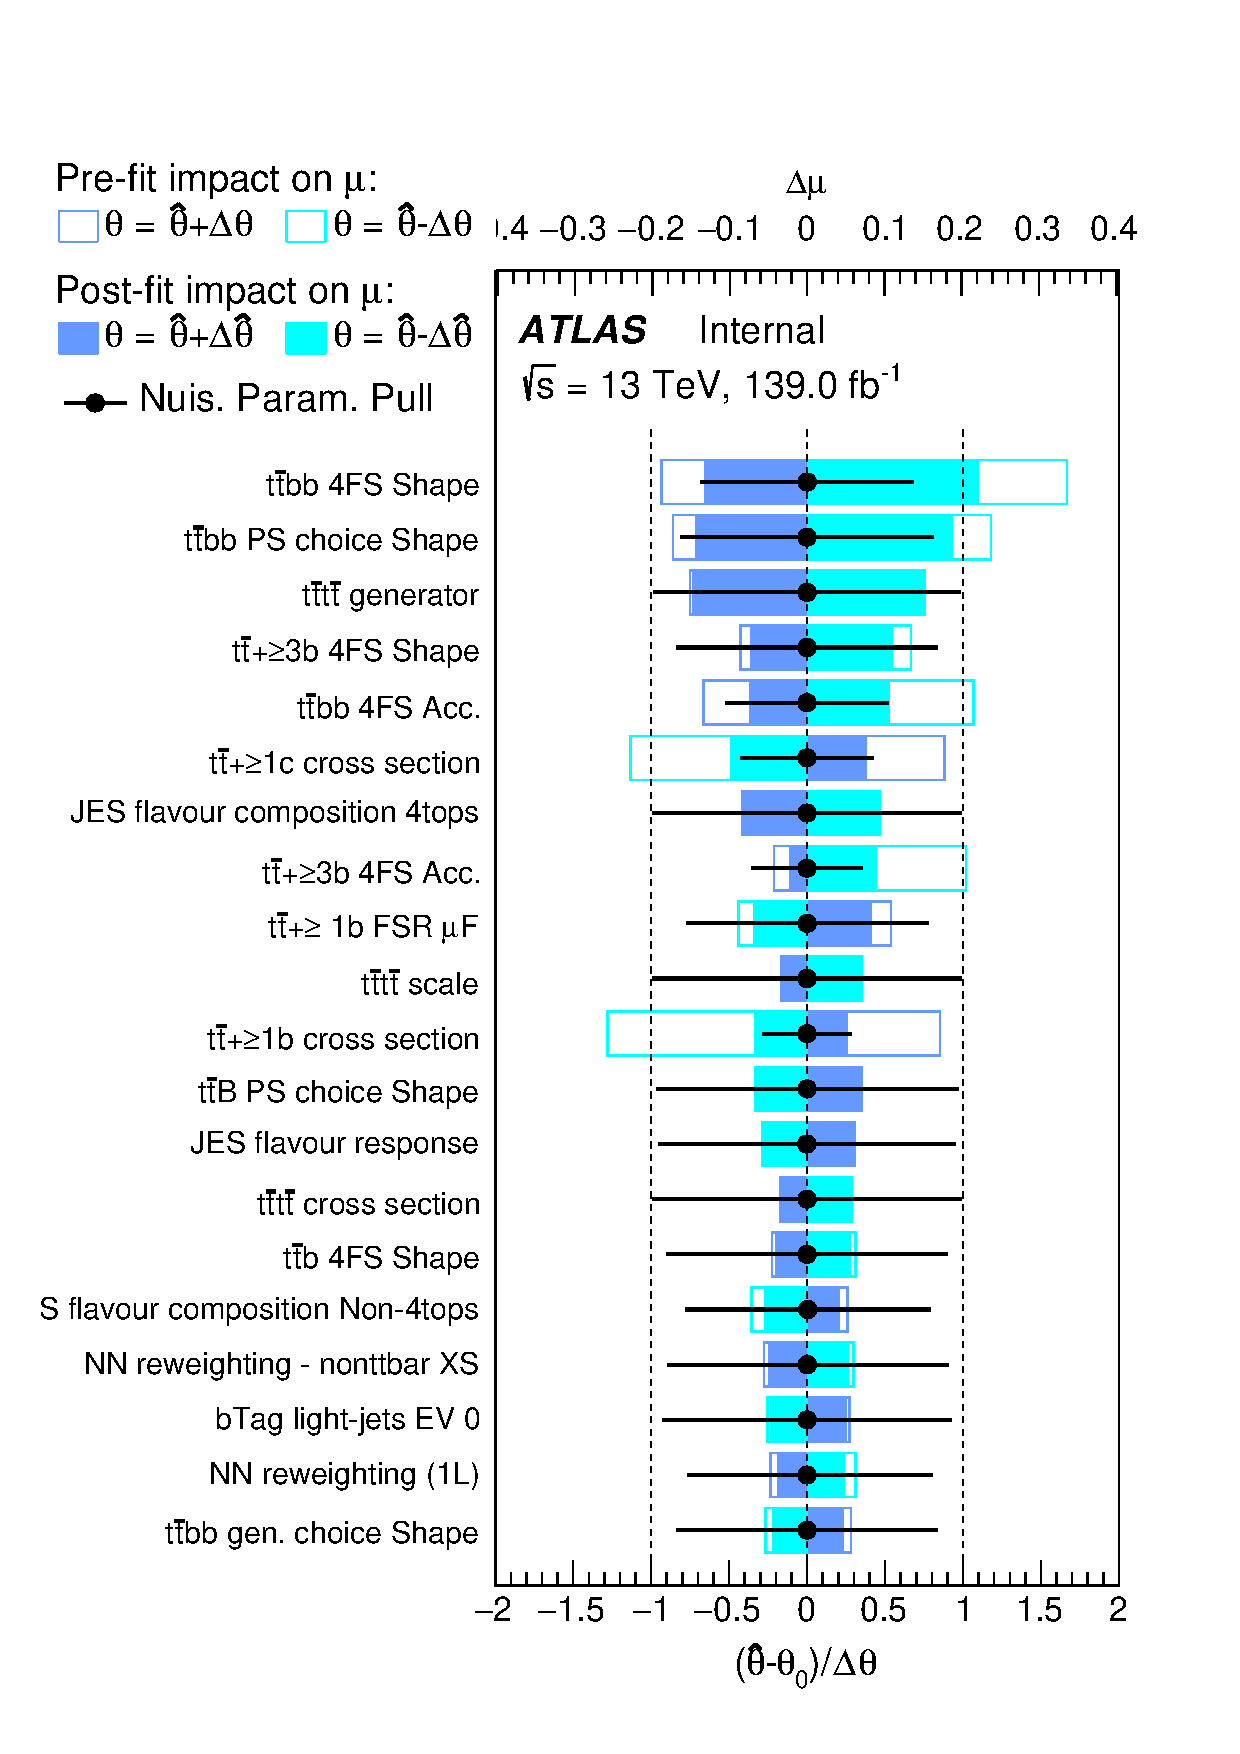
\includegraphics[width=\linewidth]{figures/fits/GNN/700/1L/asimov/Ranking_mu_tttt.pdf}
     \caption{\label{fig:Ranking_mH700_Asimov_1L}1L }
  \end{subfigure}
  \begin{subfigure}[t]{0.32\textwidth}
    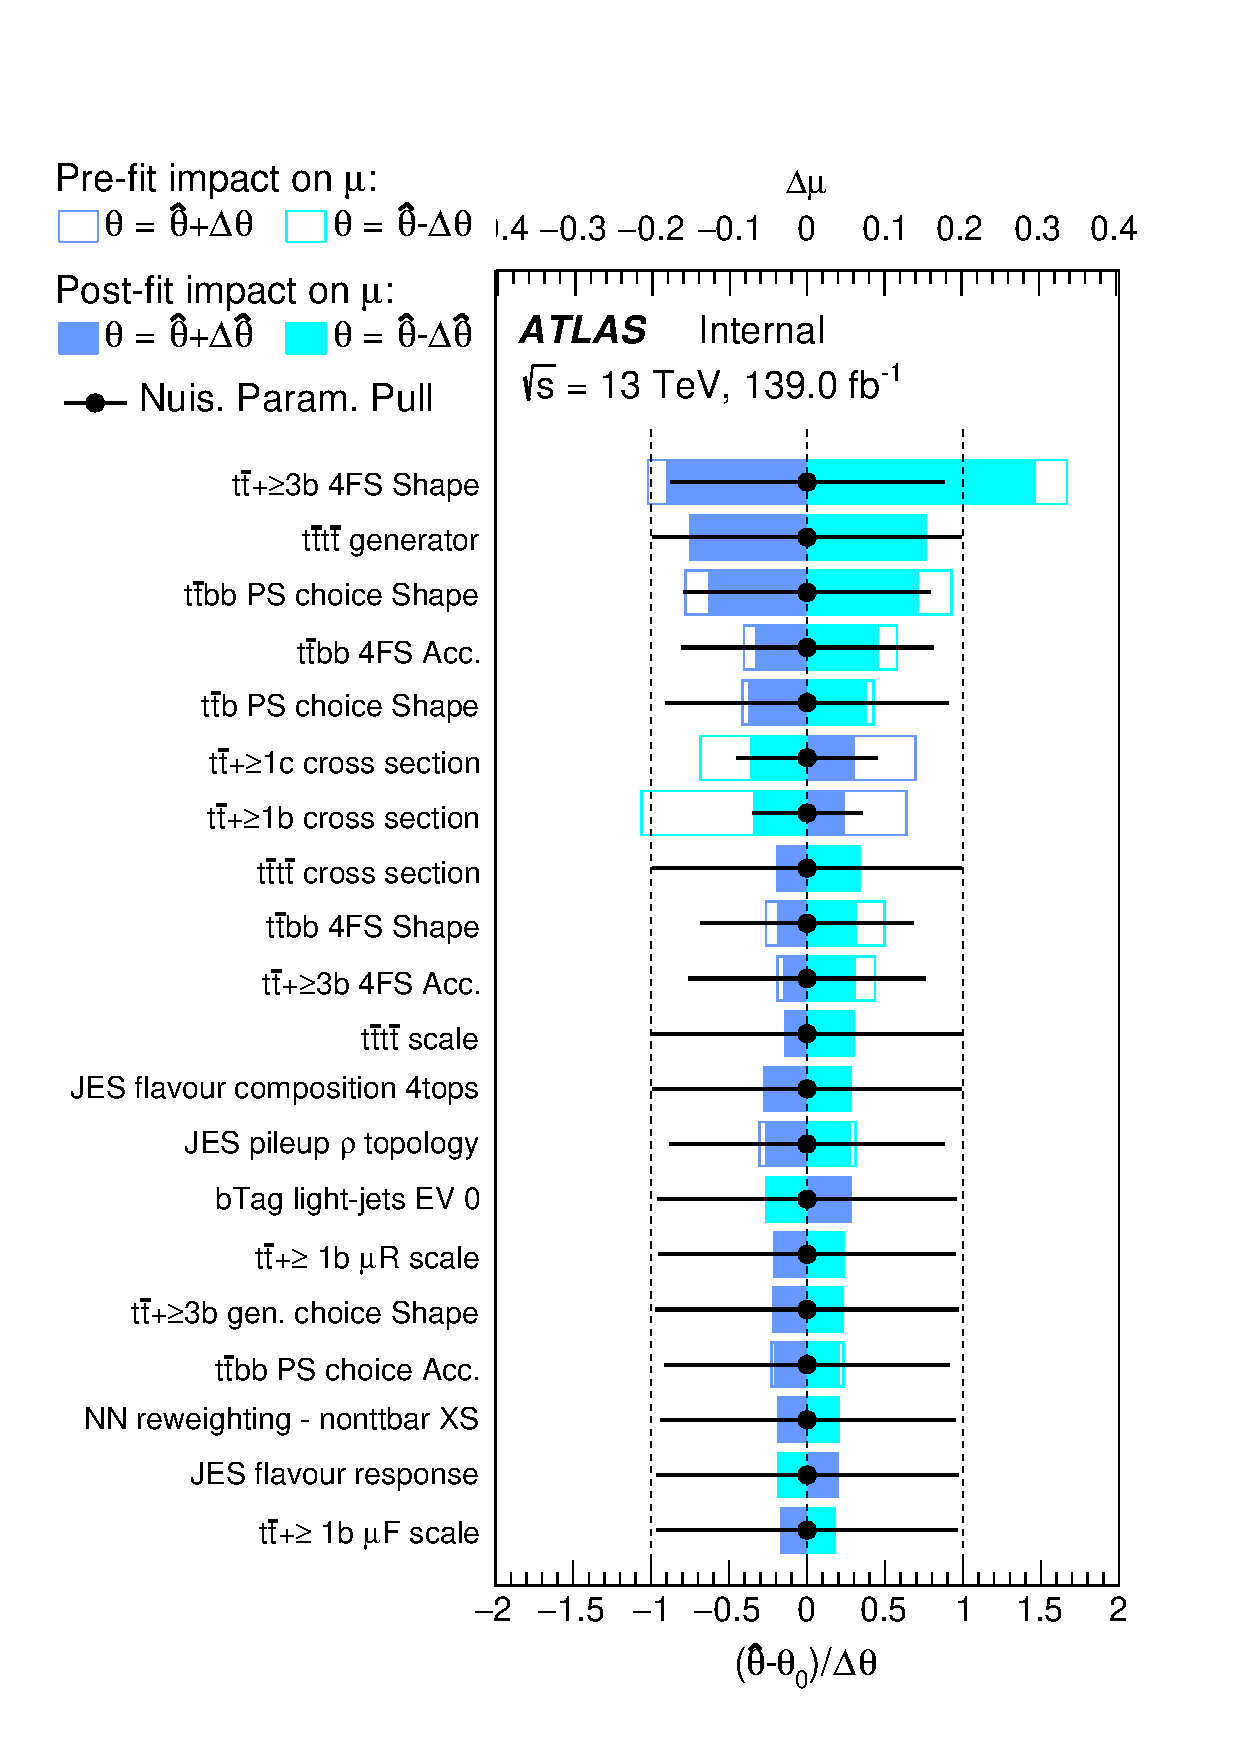
\includegraphics[width=\linewidth]{figures/fits/GNN/700/2L/asimov/Ranking_mu_tttt.pdf}
     \caption{\label{fig:Ranking_mH700_Asimov_2L}2L }
  \end{subfigure}
  \begin{subfigure}[t]{0.32\textwidth}
    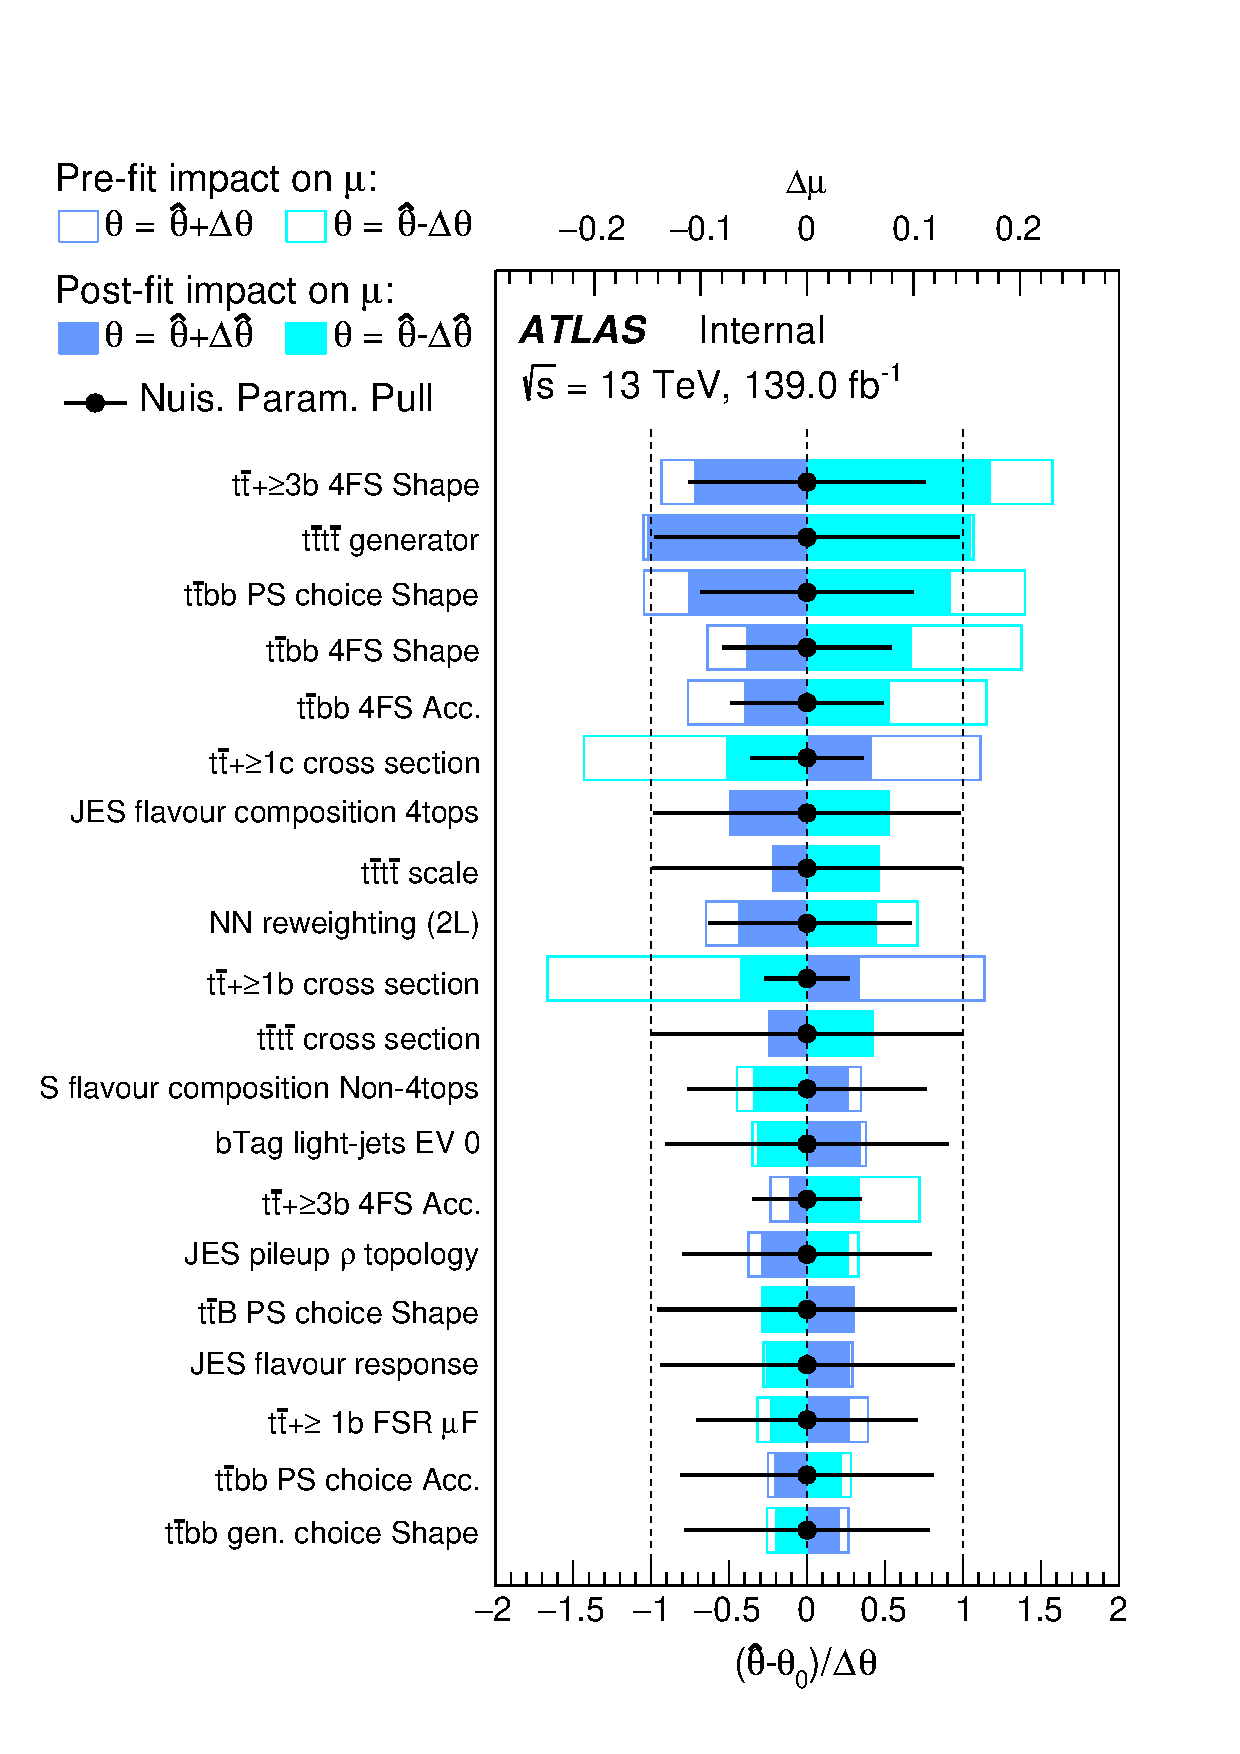
\includegraphics[width=\linewidth]{figures/fits/GNN/700/all/asimov/Ranking_mu_tttt.pdf}
     \caption{\label{fig:Ranking_mH700_Asimov_all}1L+2L }
  \end{subfigure}
  \caption{\label{fig:Ranking_mH700_Asimov}Fitted pulls and constraints for the nuisance parameters ranked by their impact for mH=700\gev for three types of Asimov fit: using only 1L regions, using only 2L regions and using all regions.}
\end{figure}

\begin{figure}[htbp!]
  \centering
  \begin{subfigure}[t]{0.32\textwidth}
    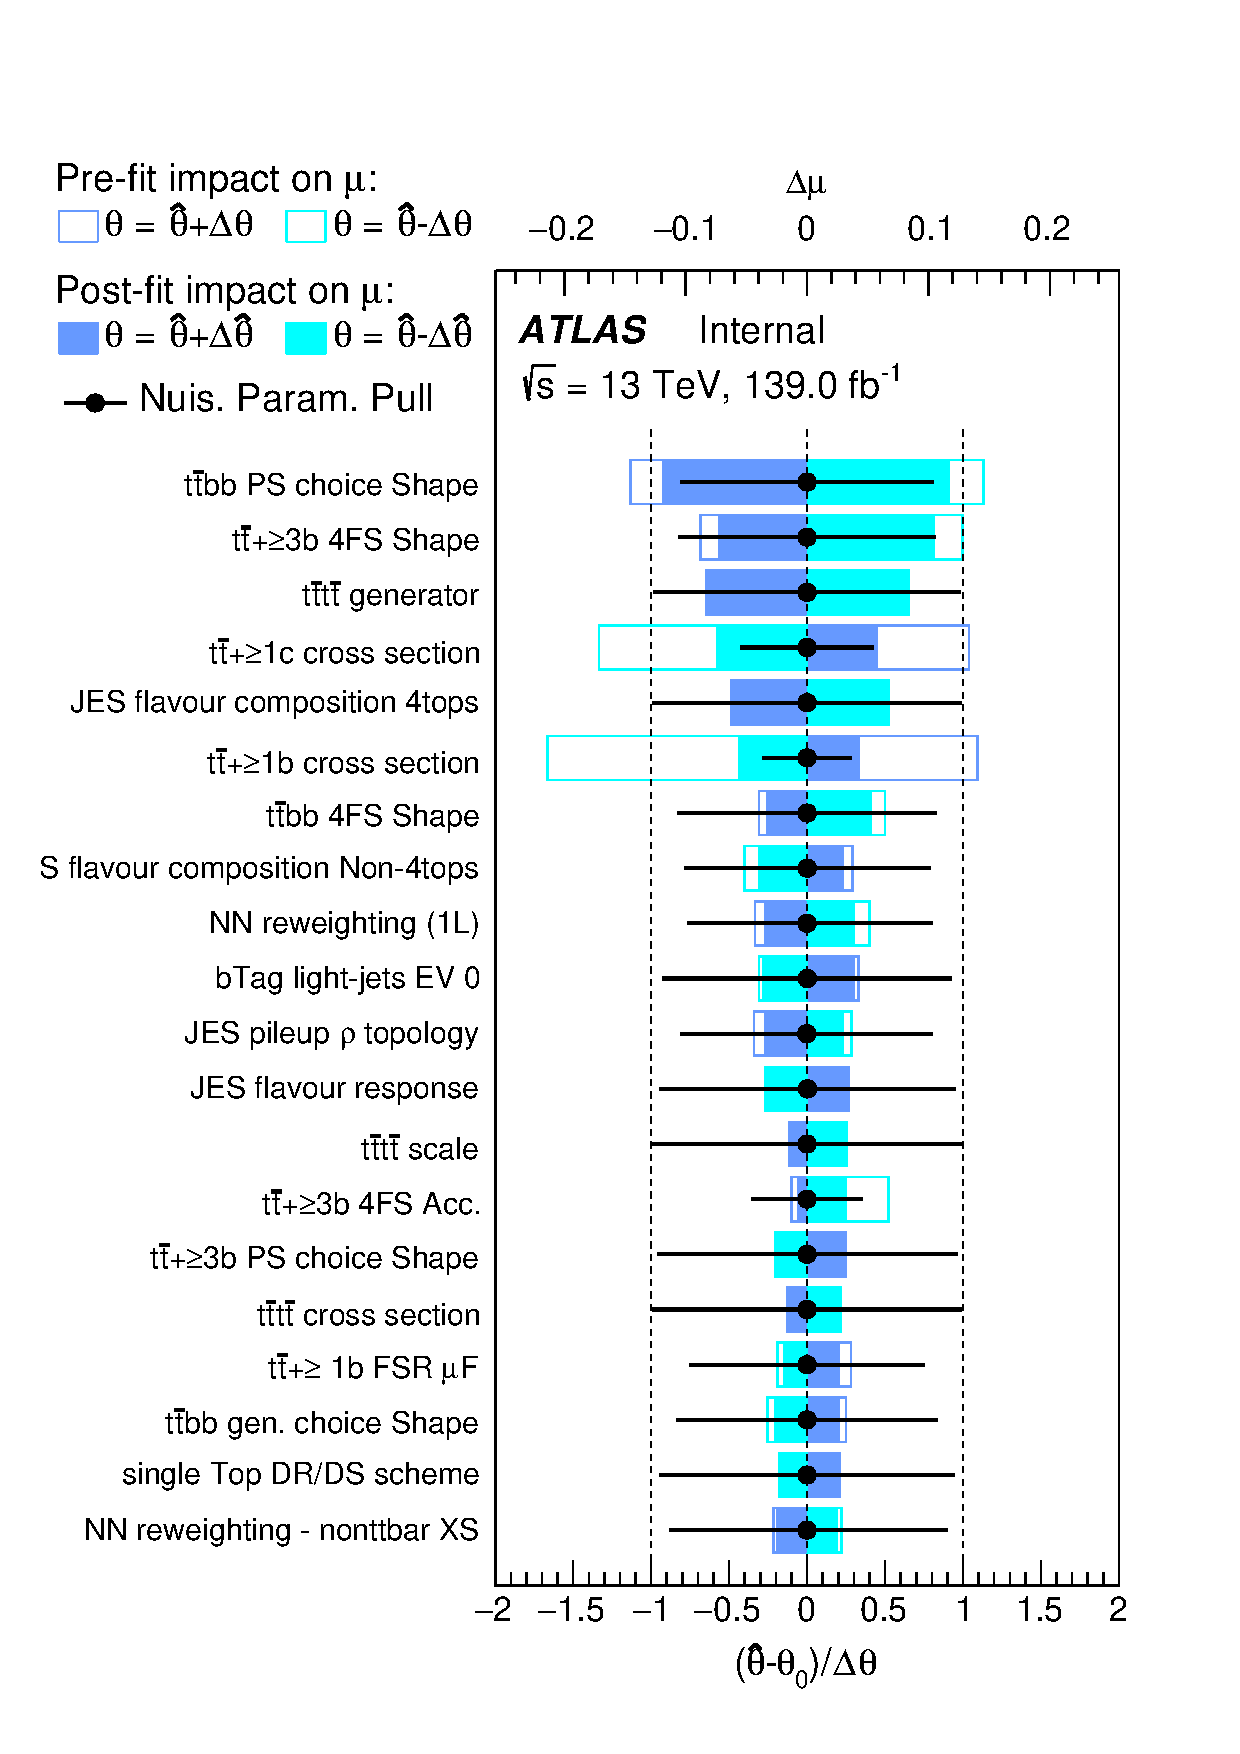
\includegraphics[width=\linewidth]{figures/fits/GNN/1000/1L/asimov/Ranking_mu_tttt.pdf}
     \caption{\label{fig:Ranking_mH1000_Asimov_1L}1L }
  \end{subfigure}
  \begin{subfigure}[t]{0.32\textwidth}
    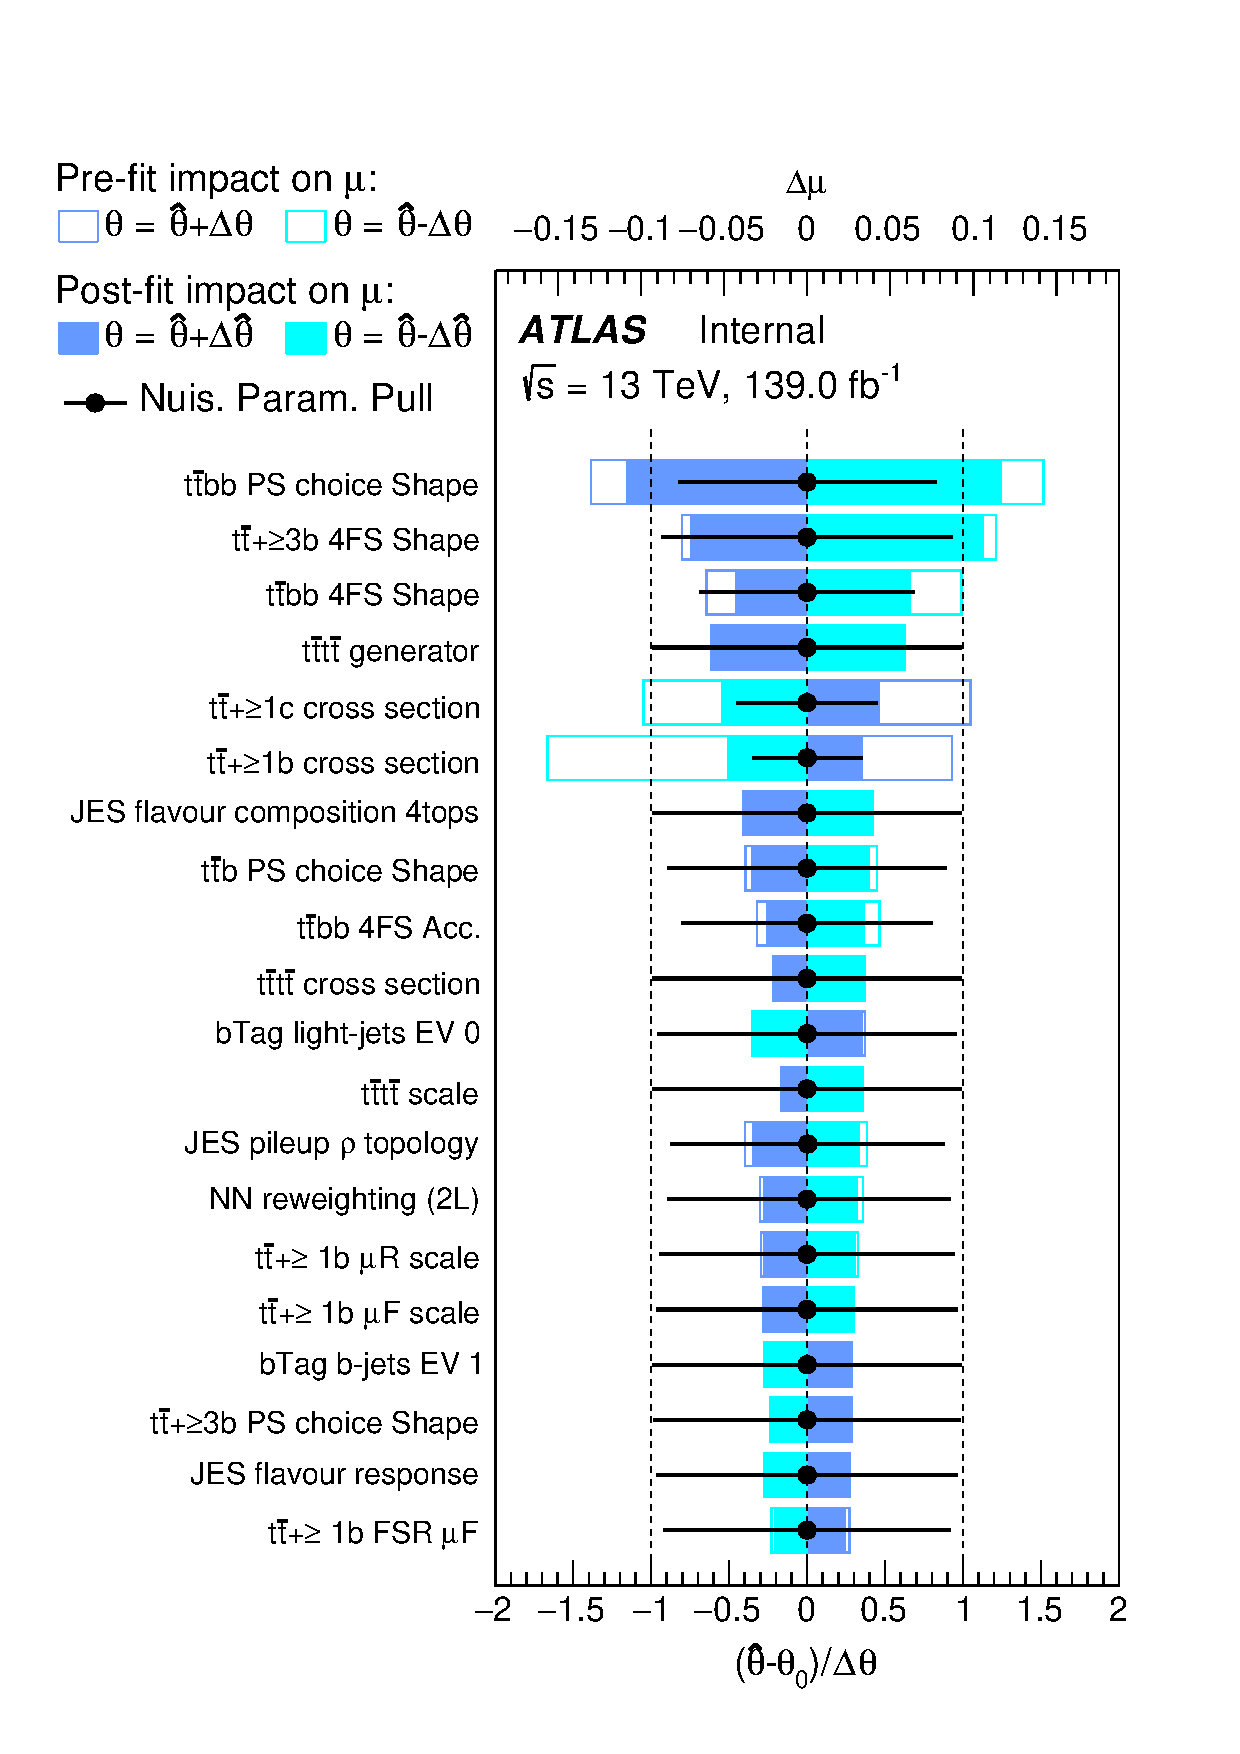
\includegraphics[width=\linewidth]{figures/fits/GNN/1000/2L/asimov/Ranking_mu_tttt.pdf}
     \caption{\label{fig:Ranking_mH1000_Asimov_2L}2L }
  \end{subfigure}
  \begin{subfigure}[t]{0.32\textwidth}
    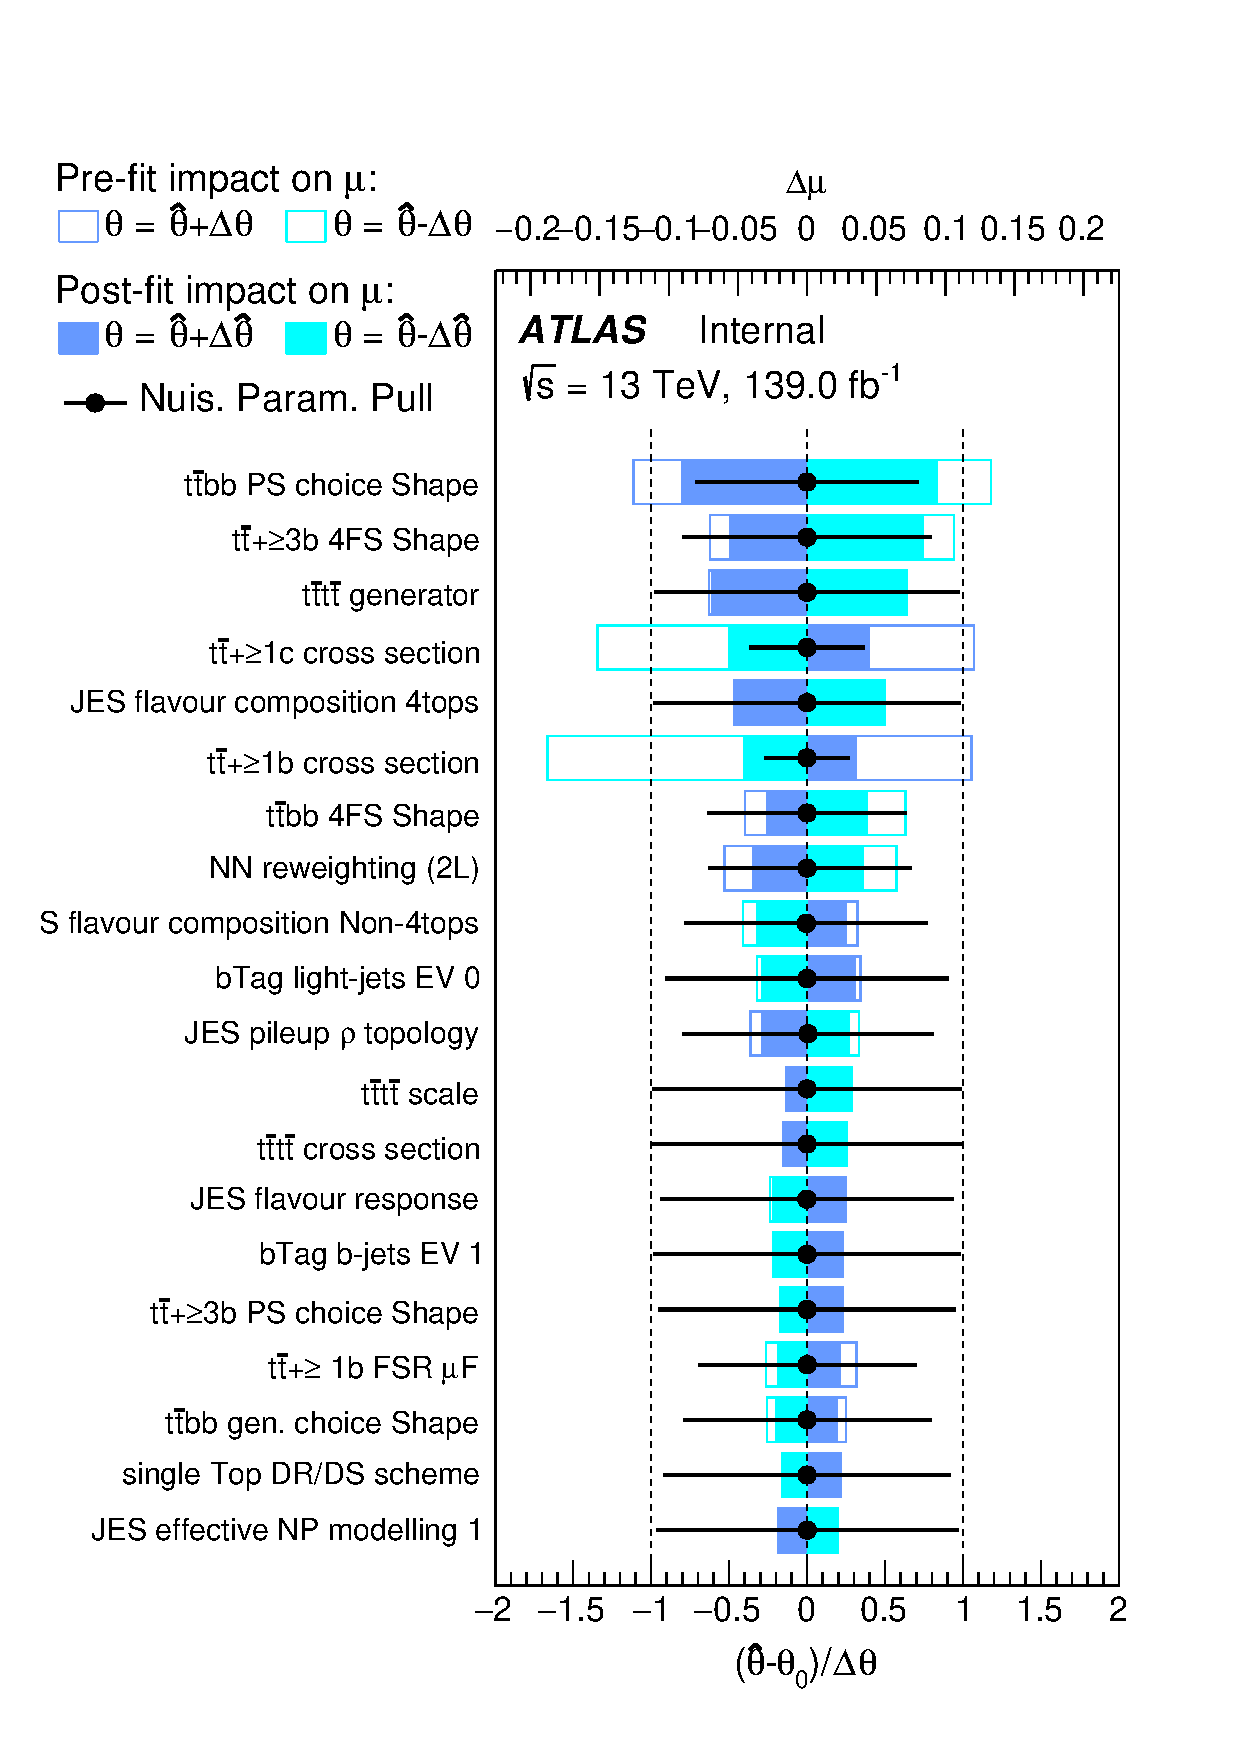
\includegraphics[width=\linewidth]{figures/fits/GNN/1000/all/asimov/Ranking_mu_tttt.pdf}
     \caption{\label{fig:Ranking_mH1000_Asimov_all}1L+2L }
  \end{subfigure}
  \caption{\label{fig:Ranking_mH1000_Asimov}Fitted pulls and constraints for the nuisance parameters ranked by their impact for mH=1000\gev for three types of Asimov fit: using only 1L regions, using only 2L regions and using all regions.}
\end{figure}


%\begin{figure}[htbp!]
%  \centering
%  \begin{subfigure}[t]{0.32\textwidth}
%    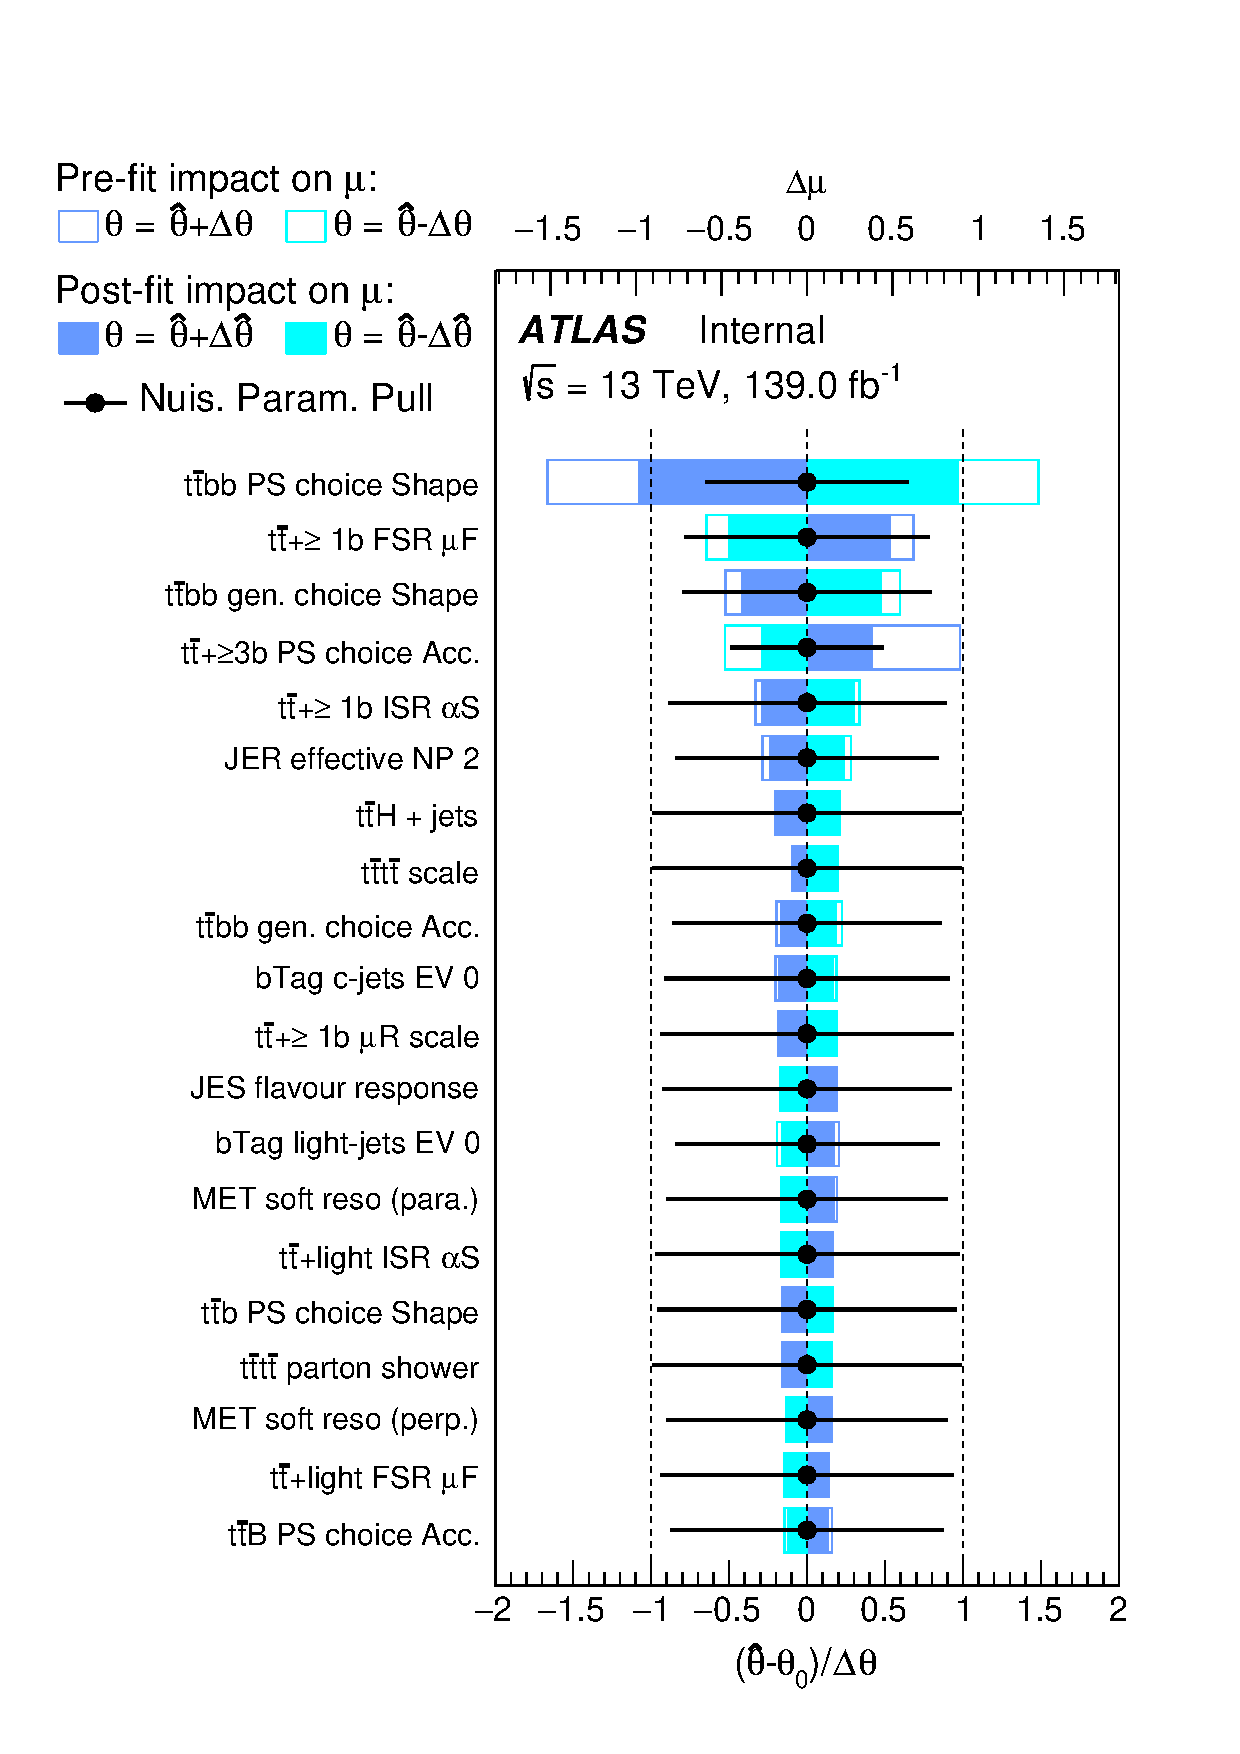
\includegraphics[width=\linewidth]{figures/fits/BDT/400/1L/asimov/Ranking_mu_tttt.pdf}
%     \caption{\label{fig:Ranking_mH400_Asimov_1L}1L }
%  \end{subfigure}
%  \begin{subfigure}[t]{0.32\textwidth}
%    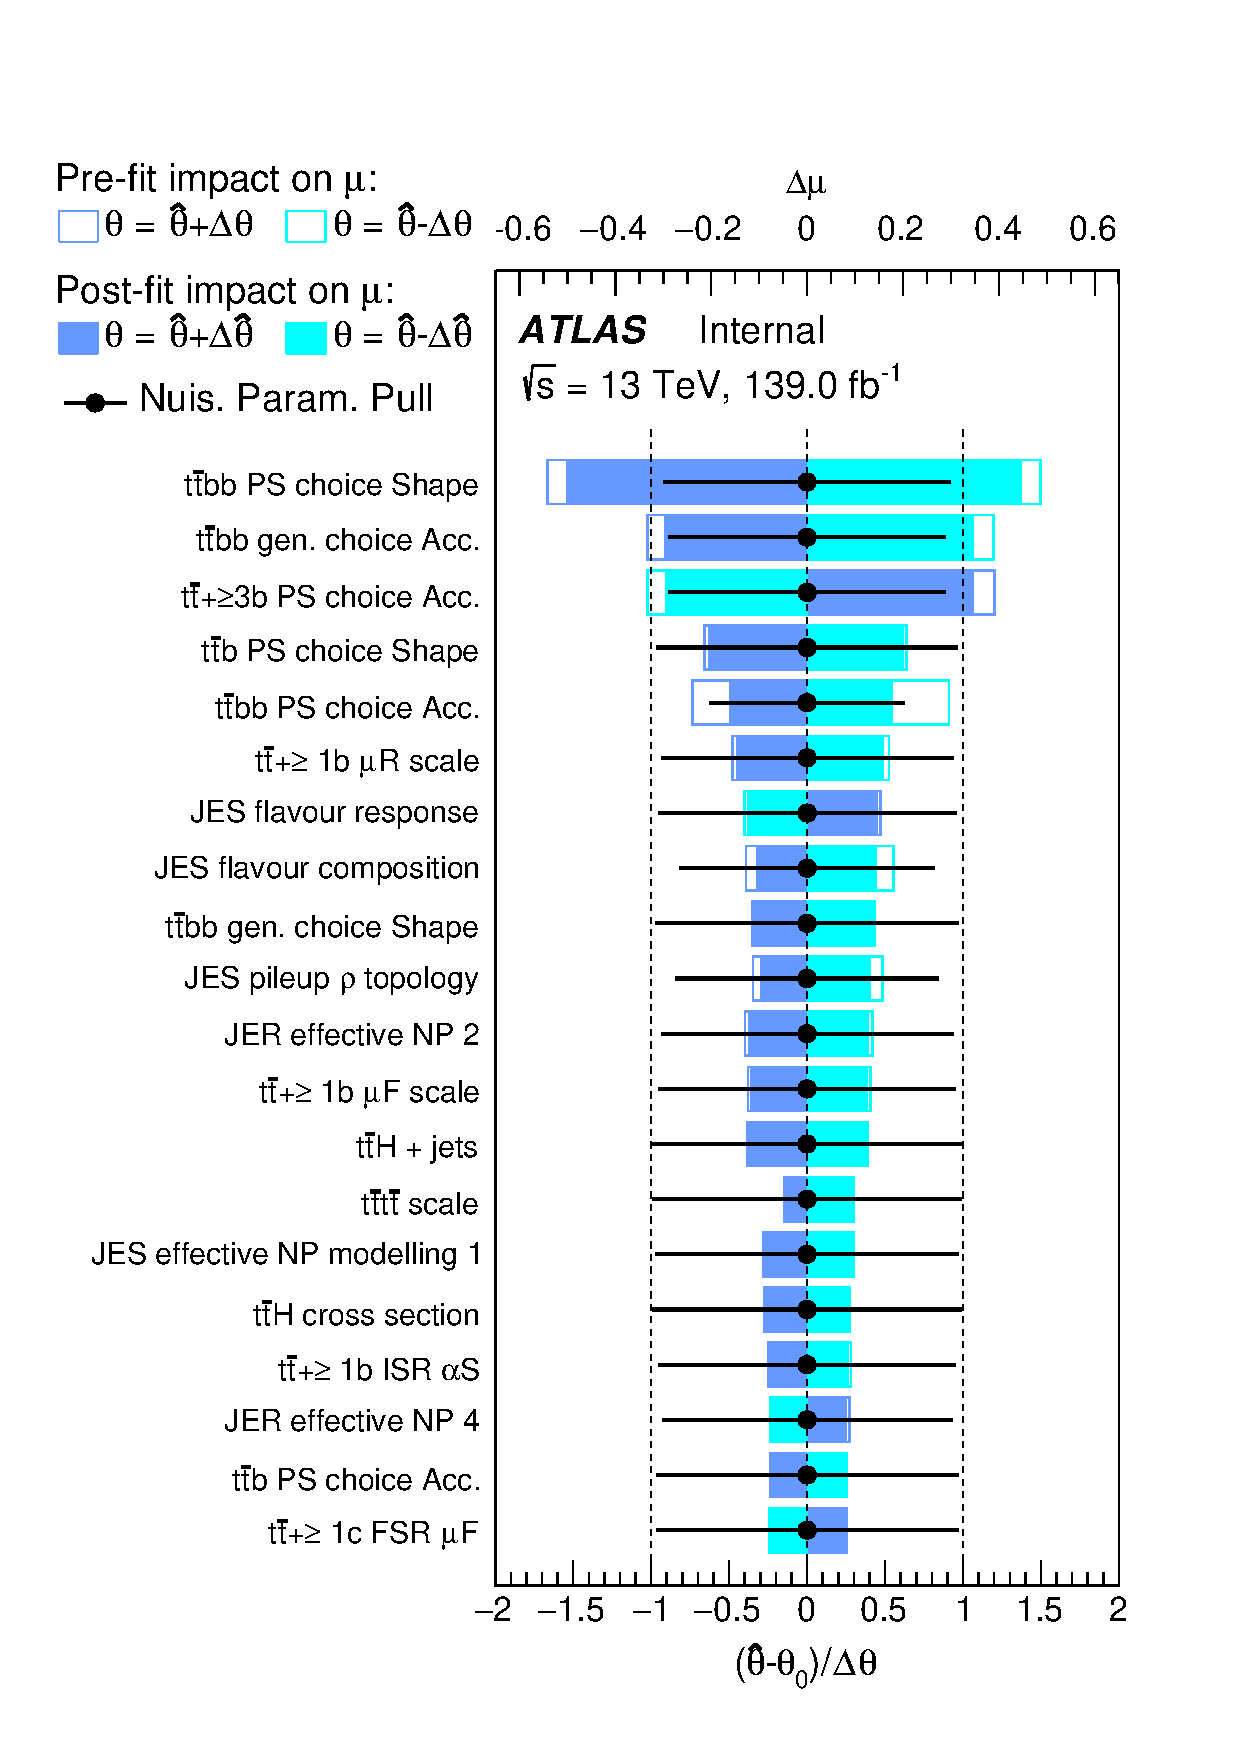
\includegraphics[width=\linewidth]{figures/fits/BDT/400/2L/asimov/Ranking_mu_tttt.pdf}
%     \caption{\label{fig:Ranking_mH400_Asimov_2L}2L }
%  \end{subfigure}
%  \begin{subfigure}[t]{0.32\textwidth}
%    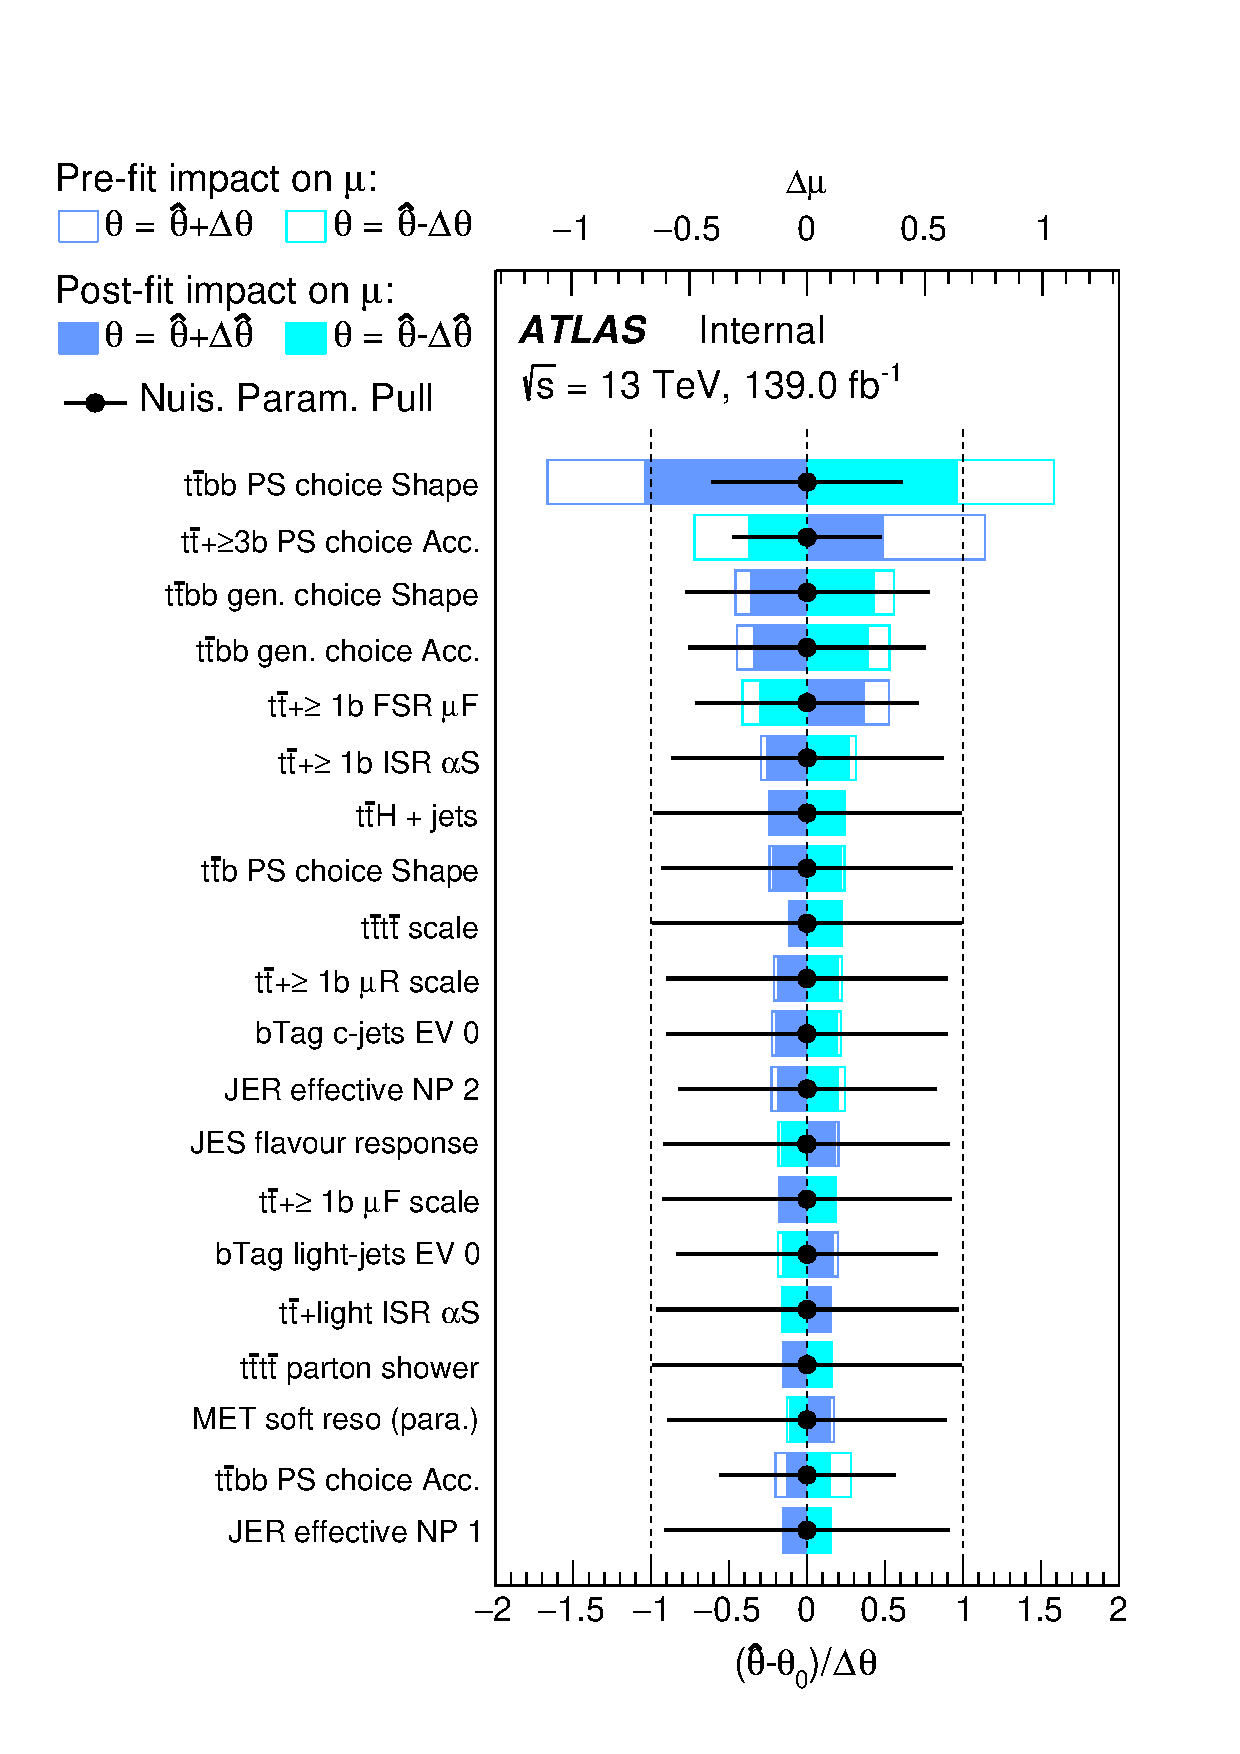
\includegraphics[width=\linewidth]{figures/fits/BDT/400/all/asimov/Ranking_mu_tttt.pdf}
%     \caption{\label{fig:Ranking_mH400_Asimov_all}1L+2L }
%  \end{subfigure}
%  \caption{\label{fig:Ranking_mH400_Asimov_BDT}Fitted pulls and constraints for the nuisance parameters ranked by their impact for mH=400\gev for three types of Asimov fit: using only 1L regions, using only 2L regions and using all regions. These fits use the BDT output distribution for the signal regions as opposed to the above fits which use GNN.}
%\end{figure}




\begin{figure}[htbp!]
        \centering
        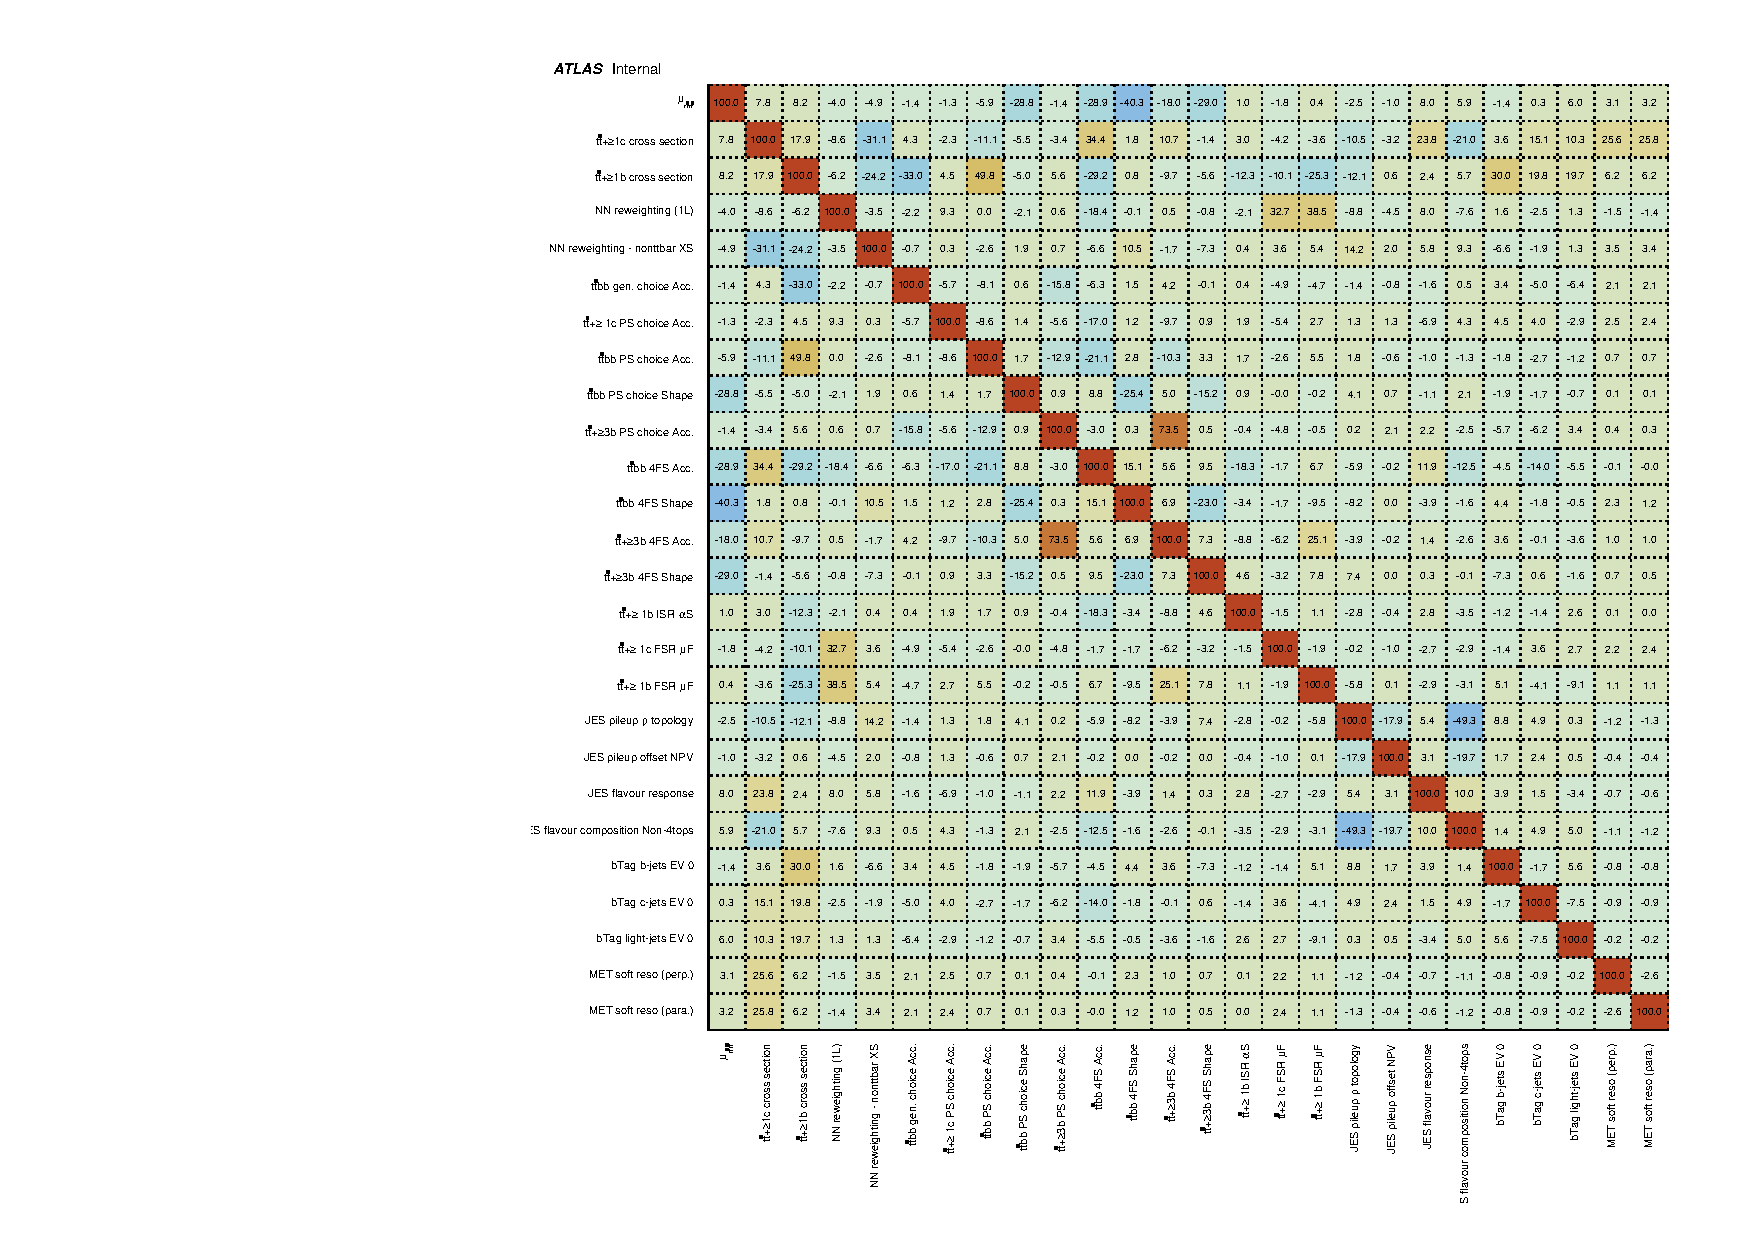
\includegraphics[width=\linewidth]{figures/fits/GNN/400/1L/asimov/CorrMatrix.pdf}
        \caption{\label{fig:Corr_mH400_Asimov_1L}Correlation matrix for the 1L Asimov fit for mH = 400 GeV}
\end{figure}

\begin{figure}[htbp!]
        \centering
        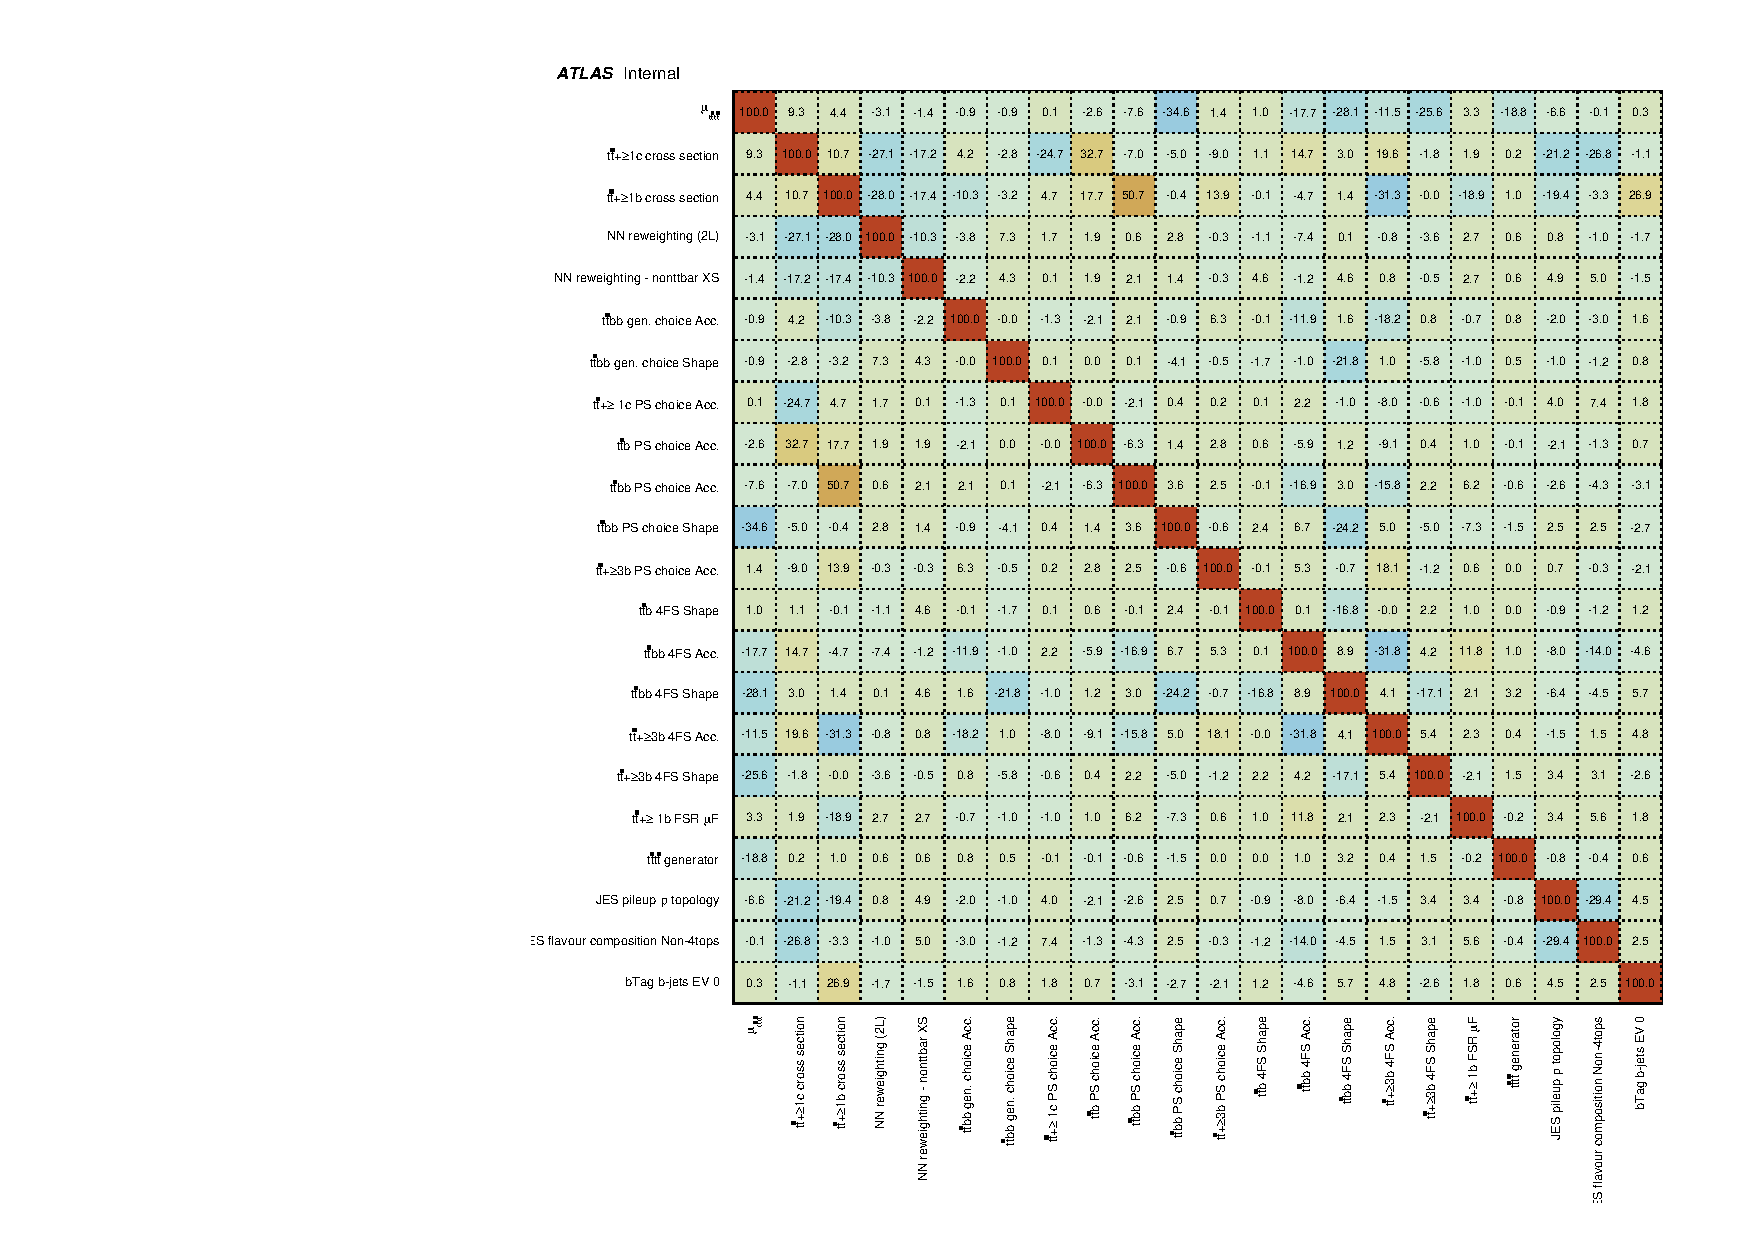
\includegraphics[width=\linewidth]{figures/fits/GNN/400/2L/asimov/CorrMatrix.pdf}
        \caption{\label{fig:Corr_mH400_Asimov_2L}Correlation matrix for the 2LOS Asimov fit for mH = 400 GeV}
\end{figure}

\begin{figure}[htbp!]
        \centering
        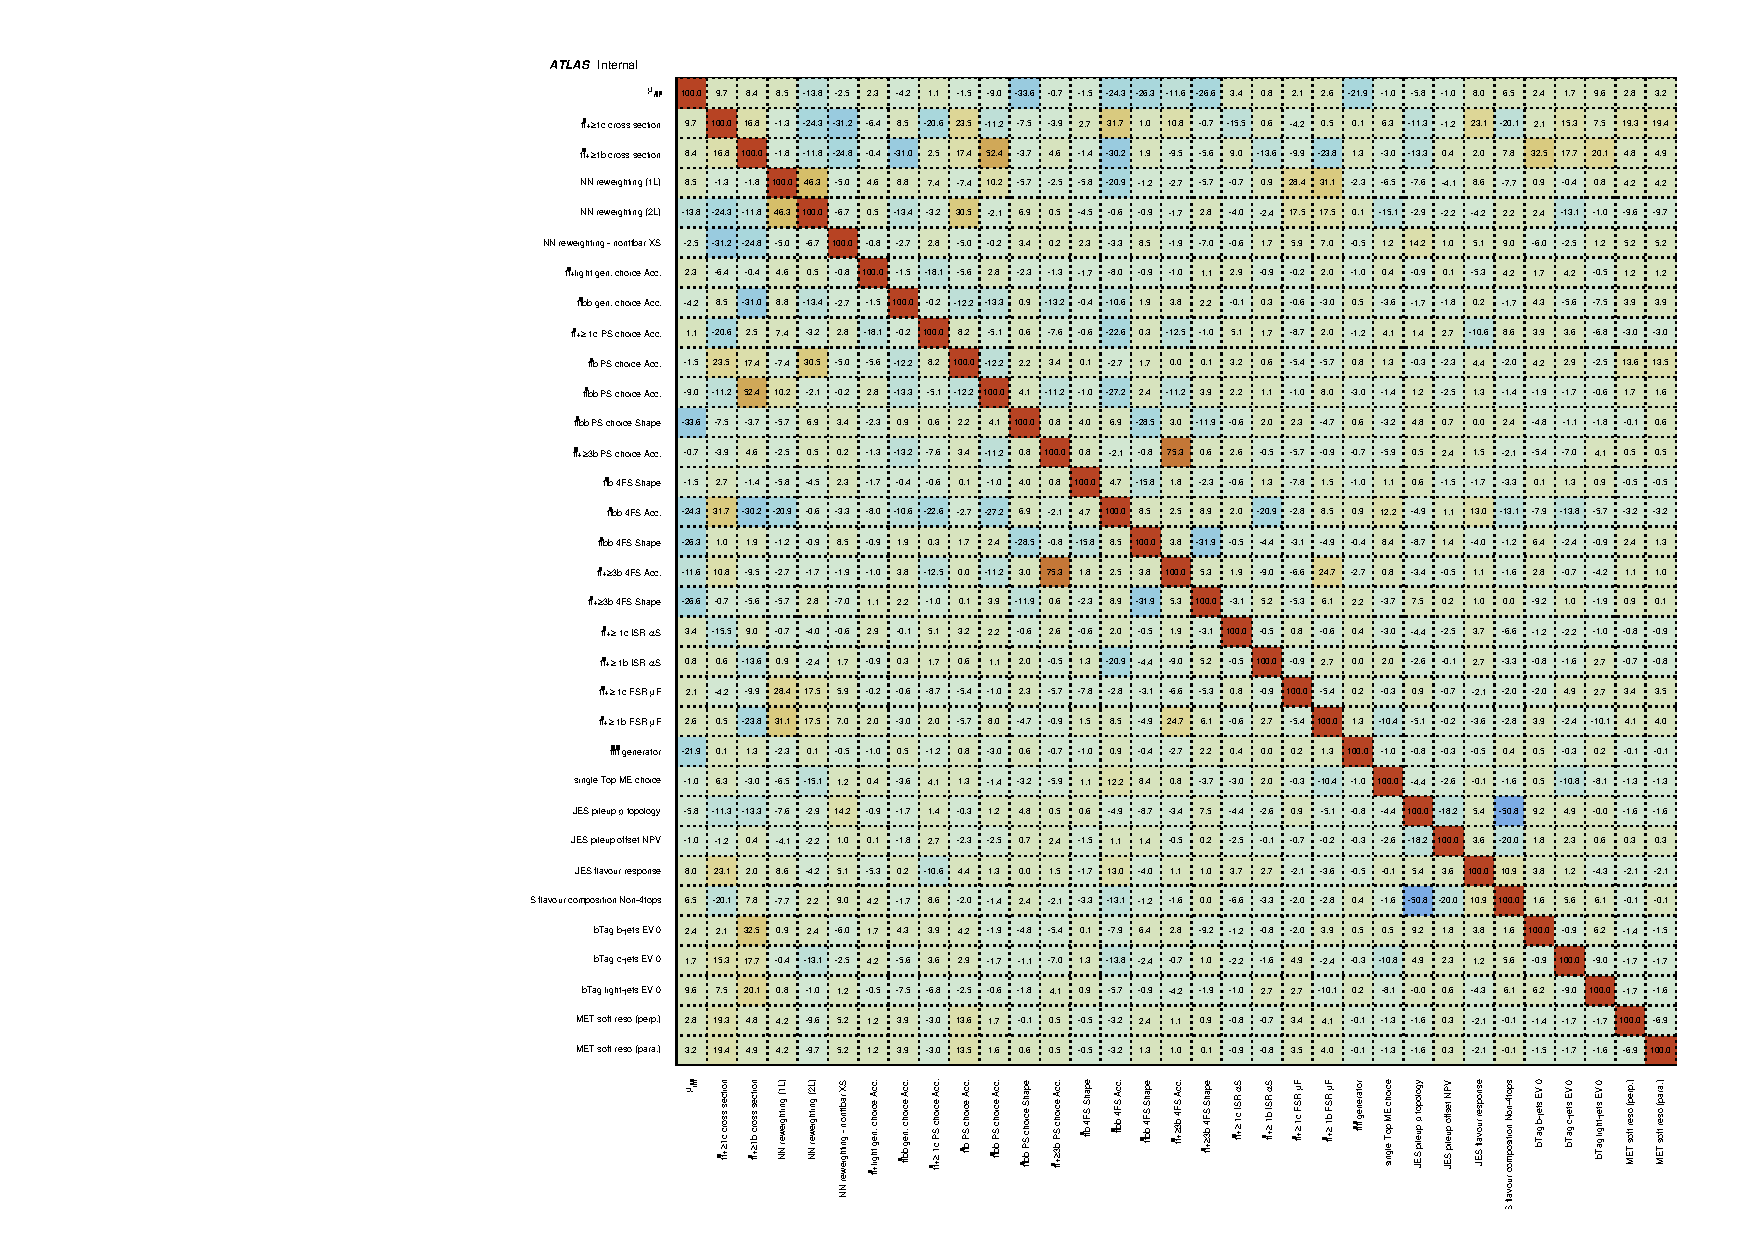
\includegraphics[width=\linewidth]{figures/fits/GNN/400/all/asimov/CorrMatrix.pdf}
        \caption{\label{fig:Corr_mH400_Asimov_all}Correlation matrix for the 1L/2LOS combined Asimov fit for mH = 400 GeV}
\end{figure}

